\chapter{VMEC}

\FloatBarrier
\section{Initial Guess for Boundary}
This section goes into the detail of how the (initial guess for) the geometry
of the last closed flux surface, which is the computational boundary in VMEC,
is specified in the input file and how this translates into the VMEC-internal array format.
In case of a fixed-boundary VMEC run, the boundary is taken as specified in the input file.
In case of a free-boundary VMEC run, the boundary specified in the input file
is taken as an initial guess and it evolves along with the geometry of the other flux surfaces.
The boundary geometry is specified using the arrays \code{rbc} and \code{zbs}
in case of a (stellarator-)symmetric case. For an asymmetric case,
additional arrays \code{rbs} and \code{zbc} can be specified.
First, consider an axisymmetric case. The configuration has no toroidal variation
and therefore, only a single Fourier mode in the toroidal direction,
namely the DC offset component at $n=0$, is required.
The magnetic axis has no poloidal variation and thus, only a single Fourier mode,
namely the DC offset at $m=0$ is required to describe its geometry.
If furthermore up/down symmetry is assumed in the axisymmetric case,
the axis has to be located at the $z=0$ plane and its geometry is then specified
by a single number, namely its radial position specified by $\hat{R}^\mathrm{cc}_{0,0}$.

\FloatBarrier
\section{Magnetic Field Representation}
The contravariant magnetic field components in VMEC are defined as follows:
\begin{align}
  B^\theta =&\, \frac{\Phi'}{\sqrt{g}} \left( \iota - \lambda_\zeta  \right)
           =    \frac{1}{\sqrt{g}} \left( \chi' - \Phi' \lambda_\zeta  \right) \label{eqn:bsuptheta} \\
  B^\zeta  =&\, \frac{\Phi'}{\sqrt{g}} \left(   1   + \lambda_\theta \right) \label{eqn:bsupzeta} \, .
\end{align}
The covariant magnetic field components are then computed using the contravariant magnetic field components and the metric elements:
\begin{align}
  B_\theta =&\, B^\theta g_{\theta \theta} + B^\zeta g_{\theta \zeta } \label{eqn:bsubtheta_from_contra} \\
  B_\zeta  =&\, B^\theta g_{\theta \zeta } + B^\zeta g_{\zeta  \zeta } \label{eqn:bsubzeta_from_contra}  \, .
\end{align}

\FloatBarrier
\section{Radial Discretization} \label{sec:radial_discretization}
In VMEC, the radial direction is discretized into a finite number (usually denoted $n_\mathrm{s}$) of flux surfaces.
Physical quantities are represented either at radial knots on the flux surfaces (full-grid)
or half-way (in toroidal flux-space) in between these (half-grid).
The radial coordinate is the normalized toridal flux:
\begin{equation}
 s_i = \frac{\Phi_i}{\Phi_\mathrm{LCFS}} \textrm{ with } i = 0, 1, ..., (n_\mathrm{s}-1)
\end{equation}
where $\Phi_\mathrm{LCFS}$ is the toroidal magnetic flux enclosed by the last closed flux surface
and $\Phi_i$ is the toroidal magnetic flux enclosed by the $i$-th flux surface.
The positions of the radial knots are usually chosen equally-distributed in $s$, leading to:
\begin{equation}
 s_i = \frac{i}{n_\mathrm{s}-1} \textrm{ with } i = 0, 1, ..., (n_\mathrm{s}-1) \, .
\end{equation}
Furthermore, the physical quantities represented as Fourier series are split
into contributions from their even poloidal harmonics and from their odd poloidal harmonics,
were a factor of $\sqrt{s}$ is factored out of the odd poloidal harmonics.
A physical quantity $f$ is then represented as follows:
\begin{equation}
 f(s) = f_\mathrm{e}(s) + \sqrt{s} f_\mathrm{o}(s)
\end{equation}
where $f_\mathrm{e}(s)$ is the contribution from even-$m$ harmonics
and $f_\mathrm{o}(s)$ is the contribution from odd-$m$ harmonics.
Then it follows for the radial derivative of $f$:
\begin{align}
 \frac{\partial f}{\partial s}
  ~ &= \frac{\partial f_\mathrm{e}}{\partial s} + \frac{\partial}{\partial s} \left( \sqrt{s} f_\mathrm{o} \right) \nonumber \\
  ~ &= \frac{\partial f_\mathrm{e}}{\partial s} + \sqrt{s} \frac{\partial f_\mathrm{o}}{\partial s} + \frac{\partial \sqrt{s}}{\partial s} f_\mathrm{o} \nonumber \\
  ~ &= \frac{\partial f_\mathrm{e}}{\partial s} + \sqrt{s} \frac{\partial f_\mathrm{o}}{\partial s} + \frac{1}{2 \sqrt{s}} f_\mathrm{o} \, .
\end{align}
Assume now that $f$ is given on the full grid
and the radial derivative is to be computed at a half-grid position $s_{i+1/2}$.
The two neighboring full-grid positions are then $s_i$ and $s_{i+1}$.
The radial derivatives of the parity-separated contributions are computed by finite differencing separately:
\begin{align}
 \frac{\partial f_\mathrm{e}}{\partial s} \left( s_{i+1/2} \right)
   &= \left[ f_\mathrm{e}(s_{i+1}) - f_\mathrm{e}(s_i) \right] / \Delta s
    = \left( n_\mathrm{s} - 1 \right) \left[ f_\mathrm{e}(s_{i+1}) - f_\mathrm{e}(s_i) \right] \\
 \frac{\partial f_\mathrm{o}}{\partial s} \left( s_{i+1/2} \right)
   &= \left[ f_\mathrm{o}(s_{i+1}) - f_\mathrm{o}(s_i) \right] / \Delta s
    = \left( n_\mathrm{s} - 1 \right) \left[ f_\mathrm{o}(s_{i+1}) - f_\mathrm{o}(s_i) \right]
\end{align}
with $\Delta s = 1 / \left( n_\mathrm{s} - 1 \right)$.
The odd contribution at the half-grid location $f_\mathrm{o}\left( s_{i+1/2} \right)$ is computed
by averaging the values at the neighboring full-grid points:
\begin{equation}
 f_\mathrm{o}\left( s_{i+1/2} \right) = \frac{1}{2} \left[ f_\mathrm{o}(s_{i+1}) + f_\mathrm{o}(s_i) \right]
\end{equation}
Putting above results together, we arrive at the following expression for the radial derivative of $f$ at $s_{i+1/2}$:
\begin{align}
   \frac{\partial f}{\partial s} \left( s_{i+1/2} \right)
 =& \phantom{+}
   \left( n_\mathrm{s} - 1 \right)
   \left[                    \left( f_\mathrm{e}(s_{i+1}) - f_\mathrm{e}(s_i) \right)
          + \sqrt{s_{i+1/2}} \left( f_\mathrm{o}(s_{i+1}) - f_\mathrm{o}(s_i) \right) \right] \nonumber \\
 ~& + \frac{1}{4 \sqrt{s_{i+1/2}}} \left[ f_\mathrm{o}(s_{i+1}) + f_\mathrm{o}(s_i) \right] \, .
\end{align}

% TODO: reverse way is used in Compute_Currents:
% The covariant magnetic field components are on the half-grid
% and the current coefficients are to be computed on the full grid.

If products of two quantities that are defined on the full-grid
are to be interpolated onto the half-grid, the so-called product interpolation rule has to be employed~\cite{hirshman_schwenn_nuehrenberg_1990}:
\begin{equation}
  (X Y)_{j-1/2} = \frac{1}{2} \left[ (X Y)_j + (X Y)_{j-1} \right] \, . \label{eqn:product_interp}
\end{equation}

\begin{figure}[htbp]
  \centering
  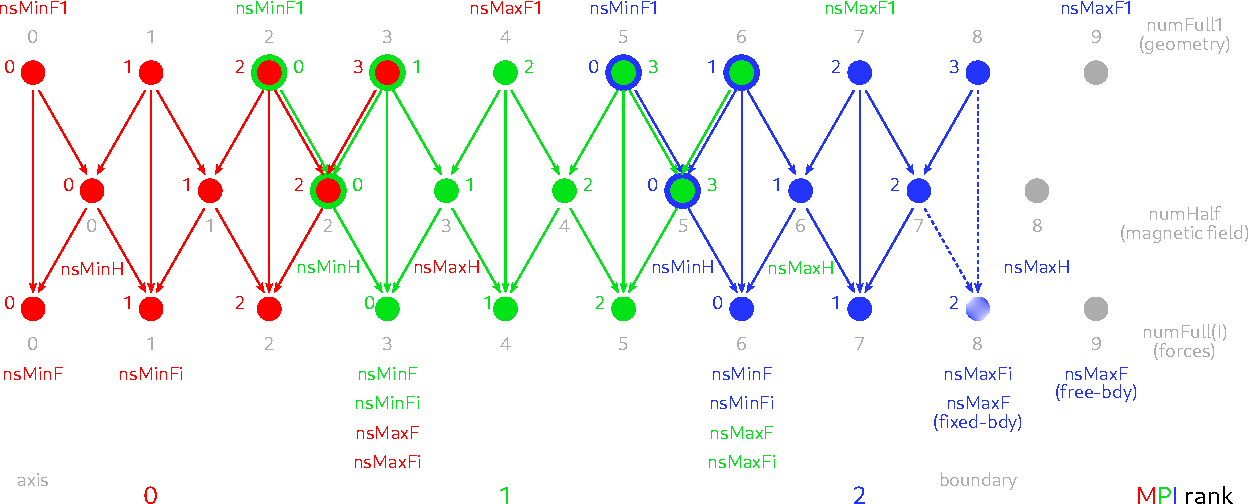
\includegraphics[width=\textwidth]{img/radial_partitioning.pdf}
  \caption{Radial partitioning scheme used in VMEC and associated MPI partitioning (colors).
           The particular example shown is for 3 MPI ranks and $\texttt{ns}=9$ flux surfaces.}
  \label{fig:vmec_radial_grids}
\end{figure}


\FloatBarrier
\section{Radial Profiles}
The distribution of flux surfaces along the radial coordinate is parameterized in VMEC via the $a^\phi$ user input polynomial,
which determines the mapping from the normalized radial coordinate $s$ (on which the flux surfaces are distributed in equal increments) to the normalized toroidal flux~$\phi$.
Thus, $a^\phi$ does not carry any physical unit.
It is specified using $n$ coefficients $a^\phi_0$, ..., $a^\phi_{n-1}$ (\code{aphi} in the input namelist).
The evaluation of the derivative of the polynomial $\phi'(s)$ at a radial location $s$ is performed using a recurrence relation starting at $i=n-1$:
\begin{equation}
  {\phi'}_{(i-1)}(s)
    \leftarrow \begin{cases}
                 n \,a^\phi_{n-1}                        &\textrm{: } i = {n-1} \\
                 s {\phi'}_{(i)}(s) + (i+1) \,a^\phi_{i} &\textrm{: else}
               \end{cases}
\end{equation}
where ${\phi'}_{(i-1)}(s)$ denotes the value of $\phi'(s)$ in the $i$-th iteration and the recurrence stops at $i=0$.
Thus, $a^\phi(s)$ specifies $\phi(s)$, but the first coefficient $a^\phi_0$ is for the term linear in $s$:
\begin{align}
              \phi(s)  =&\, a^\phi_0 s + a^\phi_1 s^2 + ... \\
  \Rightarrow \phi'(s) =&\, a^\phi_0 + 2 a^\phi_1 s + ... \, .
\end{align}
No offset is possible in $\phi(s)$ with this parameterization (and therefore always $\phi(0)=0$).
$\phi(s)$ gets computed by radially integrating ${\phi'}(s)$ using trapezoidal quadrature:
\begin{equation}
  \phi(s) = \int\limits_0^s {\phi'}(s') \,\mathrm{d}s'
    \approx \sum\limits_{i=0}^{N-1} {\phi'}({s_i}') \Delta {s_i}' \begin{cases}
                                                                    \half &\textrm{: } i=0 \textrm{ or } i=(N-1) \\
                                                                    1     &\textrm{: else}
                                                                  \end{cases}
\end{equation}
with $\Delta {s_i}' = s/N$, ${s_i}' = i \Delta {s_i}'$ and $N=100$ fixed.
The normalized poloidal flux (differential) is computed using the normalized toroidal flux (differential) and the user-provided rotational transform profile~$p_\iota(\phi_s)$.
Here is how to evaluate the normalized poloidal flux differential $\mathcal{X}'(s)$:
\begin{align}
           \phi_s =&\, \mathrm{min}\,(\phi(s, 1) \\
  \mathcal{X}'(s) =&\, p_\iota(\phi_s) {\phi'}(s) \, .
\end{align}
$\mathcal{X}(s)$ gets computed as well by radially integrating ${\mathcal{X}'}(s)$ using trapezoidal quadrature:
\begin{equation}
  \mathcal{X}(s) = \int\limits_0^s {\mathcal{X}'}(s') \,\mathrm{d}s'
    \approx \sum\limits_{i=0}^{N-1} {\mathcal{X}'}({s_i}') \Delta {s_i}' \begin{cases}
                                                                    \half &\textrm{: } i=0 \textrm{ or } i=(N-1) \\
                                                                    1     &\textrm{: else} \, .
                                                                  \end{cases}
\end{equation}
The toroidal flux enclosed by the LCFS is specified in Wb in the user input variable \code{phiedge} (denoted $\Phi_\mathrm{edge}$ here).
It is incorporated here as $\Phi_\mathrm{max}$:
\begin{equation}
  \Phi_\mathrm{max} = \frac{\code{signgs}}{2 \pi} \Phi_\mathrm{edge}
    \begin{cases}
      1/\phi(1) &\textrm{: } \phi(1) \neq 0 \\
      1         &\textrm{: else.}
    \end{cases}
\end{equation}
Note that $\phi(1)=0$ can happen, e.g., for $a^\phi_0=1$ and $a^\phi_1 = -1$.
Since $\phi(0)=0$ is fixed, $\phi(1)=0$ implies either $\phi(s)=0$ for all $s\in[0,1]$
or $\phi(s)=0$ is not monotone on $[0,1]$.
This occurs for example if an equilibrium is to be computed for a reversed-field pinch~\cite{2010_terranova, 2011_momo}.
For a Tokamak and a Stellarator, $\phi(1)=0$ is not a valid modus operandi.
The poloidal flux enclosed by the LCFS is denoted $\mathcal{X}_\mathrm{max}$:
\begin{equation}
  \mathcal{X}_\mathrm{max} = \Phi_\mathrm{max}
    \begin{cases}
      1/\mathcal{X}(1) &\textrm{: } \mathcal{X}(1) \neq 0 \\
      1                &\textrm{: else.}
    \end{cases}
\end{equation}
With the introduction of $a^\phi$, we now have three levels of parameterizations for the radial coordinate in terms of the toroidal flux:
\begin{enumerate}
  \item $s$ is the lowest level, where an equally-spaced grid ranges from $0$ to $1$ in $n_s$ steps (and the half-grid at points in between). \\
  \item $\phi(s)$ is the normalized toroidal flux from $\phi(0)=0$ at the axis to $\phi(1)$ at the LCFS.
        This profile is parameterized by the $a^\phi$ polynomial. It does not have a physical unit.
        Its value is (in the use further down) limited to $1$ and then
        used to evaluate the radial profile functions for mass, rotational transform and net toroidal current. \\
  \item $\Phi(s)$ is the physical toroidal magnetic flux enclosed in a given flux surface.
        For a Stellarator or a Tokamak we have:
        \begin{equation}
          \Phi(s) = \Phi(\phi(s)) = \frac{\code{signgs}}{2 \pi} \Phi_\mathrm{edge} \frac{\phi(s)}{\phi(1)} \, .
        \end{equation}
\end{enumerate}
The profiles of $\Phi'$, $\chi'$ and $\iota$ as well as toroidal current $I^\zeta$ are initialized on the half-grid as follows:
\begin{align}
  \Phi'_{j-\half} =&\, \Phi_\mathrm{max} \phi'(s_{j-\half}) \\
  \chi'_{j-\half} =&\, \Phi_\mathrm{max} \mathcal{X}'(s_{j-\half}) \\
  \iota_{j-\half} =&\, p_\iota    (\phi_{j-\half}) \\
I^\zeta_{j-\half} =&\, p_{I^\zeta}(\phi_{j-\half})
\end{align}
with $\phi_{j-\half} = \mathrm{min}\,(\phi(s_{j-\half}, 1)$ and $j \in \{ 1, 2, ..., (n_s-1) \}$.
The toroidal flux differential is extrapolated to the first half-grid position outside the LCFS:
\begin{equation}
  \phi_{n_s+\half} = 2 \phi_{n_s-\half} - \phi_{n_s-\nicefrac{3}{2}} \, .
\end{equation}
A scaling factor for $\lambda$ is derived from the toroidal flux differential profile:
\begin{equation}
  \lambda_\mathrm{scale} = \sqrt{\frac{1}{n_s-1} \sum\limits_{j=1}^{n_s-1} \left( \Phi'_{j-\half} \right)^2} \, . \label{eqn:lamscale}
\end{equation}
This scaling factor must not be zero, which would otherwise imply $\Phi'(s)=0$ everywhere.
It is noted that this quantity (called \texttt{lamscale} in the code)
is the RMS value of the radial profile of $\Phi'$.
%
The geometry of the LCFS is checked for compatibility with the assumed sign of the Jacobian compiled into VMEC (\code{signgs} or \code{isigng}).
If the sign of the $\theta$ coordinate needs to be flipped, this change also has to be incorporated into the profiles of $\iota$ and $\chi$:
\begin{align}
  \iota_{j-\half} \leftarrow&\, -\iota_{j-\half} \\
  \chi'_{j-\half} \leftarrow&\, -\chi'_{j-\half} \, .
\end{align}
The profiles of $\Phi'$, $\chi'$ and $\iota$ are initialized on the full-grid as follows:
\begin{align}
  \Phi'_{j} =&\, \Phi_\mathrm{max} \phi'(s_{j}) \\
  \chi'_{j} =&\, \Phi_\mathrm{max} \mathcal{X}'(s_{j}) \\
  \iota_{j} =&\, p_\iota    (\phi_{j})
\end{align}
with $\phi_{j} = \mathrm{min}\,(\phi(s_{j}, 1)$ and $j \in \{ 0, 1, ..., (n_s-1) \}$.

Note that the user-provided profiles for mass, rotational transform and net toroidal current $p_m$, $p_\iota$ and $p_{I^\zeta}$, respectively,
are always evaluated at a normalized toroidal flux coordinate ranging from $0$ at the magnetic axis to $1$ at the LCFS.
Thus, the re-distribution of flux surfaces using the $a^\phi$ polynomial
can be performed without changing the assumed coordinate of the prescribed profiles.

The Jacobian $\sqrt{g}$ is available on the radial half-grid.
This allows to compute the differential volume profile $V'(s)$
where $V$ is the volume enclosed by a given flux surface and the prime denotes a derivative with respect to $s$ (see Eqn.~(4.9.10) in Ref.~\cite{dHaseleer}):
\begin{equation}
  V'(s) = \frac{\mathrm{d}V}{\mathrm{d}s}(s) = \int\limits_0^{2 \pi} \int\limits_0^{2 \pi} \sqrt{g}(s, \theta, \zeta) \,\mathrm{d}\theta \,\mathrm{d}\zeta \, .
\end{equation}
In VMEC, the sign of the Jacobian $\sqrt{g}$ is usually negative and thus, the absolute value of $\sqrt{g}$ should be taken
for computing the (differential) plasma volume; $\sqrt{g}$ is to be regarded as a symbol and throughts should be prevented to wander into considering imaginary volumes.
In VMEC, the differential volume is computed on the half-grid as follows:
\begin{align}
        ~&\, \frac{1}{(2 \pi)^2} V'(s_{j-\half}) = \code{vp}(s_{j-\half}) \nonumber \\
        =&\, \frac{1}{(2 \pi)^2}\int\limits_0^{2 \pi} \int\limits_0^{2 \pi} |\sqrt{g}(s_{j-\half}, \theta, \zeta)| \,\mathrm{d}\theta \,\mathrm{d}\zeta \nonumber \\
  \approx&\, \frac{1}{(2 \pi)^2}\sum\limits_{k=0}^{n_\theta - 1} \sum\limits_{l=0}^{n_\zeta - 1} |\sqrt{g}(s_{j-\half}, \theta_k, \zeta_l)| \Delta \theta \Delta \zeta \nonumber \\
        =&\, \frac{1}{\bcancel{(2 \pi)^2}} \frac{\bcancel{2 \pi}}{n_\theta} \frac{\bcancel{2 \pi}}{n_\zeta}
               \sum\limits_{k=0}^{n_\theta - 1} \sum\limits_{l=0}^{n_\zeta - 1} |\sqrt{g}(s_{j-\half}, \theta_k, \zeta_l)| \nonumber \\
        =&\, \frac{1}{n_\theta n_\zeta} \sum\limits_{k=0}^{n_\theta - 1} \sum\limits_{l=0}^{n_\zeta - 1} |\sqrt{g}(s_{j-\half}, \theta_k, \zeta_l)|
\end{align}
with the following discretization in the tangential coordinates:
\begin{align}
  \Delta \theta =&\, 2 \pi / n_\theta \\
  \Delta \zeta  =&\, 2 \pi / n_\zeta  \\
  \theta_k      =&\, k \Delta \theta \\
  \zeta_l       =&\, l \Delta \zeta \, .
\end{align}
The total plasma volume is computed as follows:
\begin{align}
  V       =&\, \int\limits_0^1 V'(s) \,\mathrm{d}s \\
    \approx&\, \frac{(2 \pi)^2}{n_s-1} \sum\limits_{j=1}^{n_s - 1} \frac{V'(s_{j-\half})}{(2 \pi)^2} \\
          =&\, \frac{(2 \pi)^2}{n_s-1} \sum\limits_{j=1}^{n_s - 1} \code{vp}(s_{j-\half}) \, . \label{eqn:voli}
\end{align}
In the first iteration, the initial plasma volume is computed using~\eqn{voli} and stored in~\code{voli}.
The mass profile $m(s)$ is specified in the user input as a parameterized function $\code{pmass}(s)$,
a scaling factor \code{pres\_scale} and the adiabatic index $\gamma$:
\begin{equation}
  \mu_0 m(s_{j-\half}) = \code{mass}((s_{j-\half}))
   = \mu_0 \cdot \code{pres\_scale} \cdot \code{pmass}(s_{j-\half}) \cdot \left( |\code{vpnorm}| \cdot \code{r00} \right)^\gamma
\end{equation}
where
\begin{equation}
  \code{vpnorm} = \code{signgs} \cdot \frac{\Phi_\mathrm{LCFS}}{2 \pi} \cdot \Phi'(s_{j-\half})
\end{equation}
and $\code{r00}$ is the $R_{00}$ component of the LCFS as specified in the user input.
Given the mass profile $m(s)$, the pressure profile $p(s)$ is computed on the half-grid:
\begin{align}
  \mu_0 p(s_{j-\half}) = \code{pres}(s_{j-\half})
   =&\, \frac{\mu_0 m(s_{j-\half})}{\left( V'(s_{j-\half}) / (2 \pi)^2 \right)^\gamma} \nonumber \\
   =&\, \frac{\code{mass}(s_{j-\half})}{\left(\code{vp}(s_{j-\half})\right)^\gamma} \, .
\end{align}
For $\gamma = 0$, the pressure profile is prescribed:
\begin{equation}
  \mu_0 p(s_{j-\half}) = \mu_0 m(s_{j-\half}) = \mu_0 \cdot \code{pres\_scale} \cdot \code{pmass}(s_{j-\half}) \, .
\end{equation}
Two typical use cases are found:
\begin{itemize}
  \item $\code{pmass}(s)$ specified a normalized pressure profile with $p(0) = 1$ at the magnetic axis and $p(1) = 0$ at the LCFS.
        \code{pres\_scale} then scales this profile to a given physical pressure, e.g., 10\,kPa.
  \item $\code{pmass}(s)$ specified a physical pressure profile in Pa, e.g., from measurements and
        \code{pres\_scale} scales this profile by a small factor (say $0.5 \leq \code{pres\_scale} \leq 2$)
        to study the influence of a global change in plasma pressure on some subsequent physical quantity
        obtained from the equilibrium output.
\end{itemize}

\FloatBarrier
\section{Real-Space Grid Setup}
For up/down-symmetric two-dimensional configurations
and for Stellarator-symmetric three-dimensional configurations,
use can be made of the parity of the basis functions
to reduce the computational work by a factor of ca.~2.
This is done by computing quantities only on half the poloidal domain.
The choice to make use of parity in the poloidal direction
vs. the toroidal direction is gouverned by the fact
that this way, also axisymmetric configurations can make use of this symmetry.

The number of poloidal grid points needs to be even for this to work out.
The user-prescribed number of poloidal grid points, \texttt{ntheta},
is rounded down to the nearest even integer value:
\begin{equation}
  n_{\theta, 1} = 2 \left\lfloor \frac{\texttt{ntheta}}{2} \right\rfloor \, .
\end{equation}
If \texttt{ntheta} is not given in the input file,
the minimum value required to support the prescribed number of poloidal modes \texttt{mpol} is used.
In case of a symmetric computation,
the poloidal grid is reduced to $n_{\theta,2}$ grid points with
\begin{equation}
  n_{\theta,2} = \frac{n_{\theta, 1}}{2} + 1 \, .
\end{equation}
This is illustrated in Fig.~\ref{fig:poloidal_symmetry}.
\begin{figure}[htbp]
  \centering
  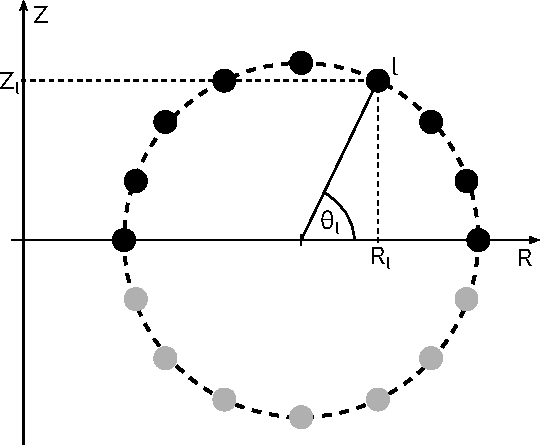
\includegraphics{img/poloidal_symmetry.pdf}
  \caption{Poloidal symmetry can be used to reduce the grid from the full $[0, 2 \pi[$ interval
  (black and grey dots) to only the symmetric half $[0, \pi]$ (black dots only).
  The $l$-th poloidal grid point at $(R_l,Z_l)$ is indicated with its poloidal coordinate~$\theta_l$.
  Here, $n_{\theta,1} = 16$ and $n_{\theta,2} = 9$.}
  \label{fig:poloidal_symmetry}
\end{figure}
If the full poloidal range is used and thus
\begin{equation}
  \theta_l = \frac{2 \pi}{n_{\theta,1}} l \textrm{ for } l = 0, 1, ..., (n_{\theta,1}-1) \, .
\end{equation}
In case use is made of symmetry, this leads to
\begin{align}
    \theta_l = \frac{2 \pi}{n_{\theta,1}} l
  =&\, \frac{\bcancel{2} \pi}{\bcancel{2}(n_{\theta,2}-1)} l \nonumber \\
  =&\, \frac{\pi}{n_{\theta,2}-1} l \textrm{ for } l = 0, 1, ..., (n_{\theta,2}-1) \, .
\end{align}
The equations to be solved are formulated using~$\phi$ as the toroidal coordinate.
Assuming discrete toroidal translation invariance over $n_\mathrm{fp}$~field periods,
quantities only need to be evaluated on the interval $\phi \in [0, 2\pi/n_\mathrm{fp}[$.
This is equivalent to evaluating them in terms of the toroidal angle per module,~$\zeta$,
on the interval~$\zeta \in [0, 2\pi[$.
Note however that toroidal derivatives are still to be taken wrt.~$\phi$
and thus a factor $n \cdot n_\mathrm{fp}$ appears in front of the Fourier coefficients.
The number of toroidal grid points, $n_\zeta$, to be used in the computation
is specified in the input variable~\texttt{nzeta}.
The discrete grid in toroidal direction consists of $n_\zeta$ points:
\begin{equation}
  \zeta_k = \frac{2 \pi}{n_\zeta} k \textrm{ for } k = 0, 1, ..., (n_\zeta-1) \, .
\end{equation}
This corresponds to a grid over one field period in the cylindrical coordinate~$\phi$:
\begin{equation}
  \phi_k = \frac{2 \pi}{n_\mathrm{fp} n_\zeta} k \textrm{ for } k = 0, 1, ..., (n_\zeta-1) \, ,
\end{equation}
leading to~$\phi_k \in [0, 2 \pi / n_\mathrm{fp}[$.

In a nutshell:
The basis function argument is~$(m \theta - n n_\mathrm{fp} \phi)$.
Evaluation of functions and their tangential derivatives is only ever done in the first toroidal period:
$\phi \in [0, 2\pi/n_\mathrm{fp}[ \Rightarrow \zeta \in [0, 2\pi[$.
Therefore, the argument $(m \theta - n \zeta)$ is used in the evaluation of the Fourier basis functions.
Toroidal derivatives are to be taken with respect to $\phi$.
The Fourier representation allows to do this analytically and a factor~$-n n_\mathrm{fp}$ comes out of the basis function.

\FloatBarrier
\section{Fourier Representation} \label{sec:vmec_fourier_transforms}
The quantites $R$, $Z$ and $\lambda$ are the state variables in VMEC that describe the solution.
These quantites are represented by two-dimensional Fourier series in $\theta$ and $\zeta$ on each of the flux surfaces.
VMEC is designed to allow computation of the MHD equilibrium for both symmetric and asymmetric two- and three-dimensional configurations.
This freedom comes at a cost.
Multi-dimensional Fourier transforms with a complex-valued Fourier basis
can easily be evaluated as a separable product over the dimensions:
\begin{equation}
  \exp(i (m \theta - n \zeta)) = \exp(i m \theta) \exp(i n \zeta) \, .
\end{equation}
The real-valued two-dimensional Fourier basis functions used in VMEC
are split up into two contributing separable products of basis functions to be added up:
\begin{align}
  \cos(m \theta - n \zeta) =& \cos(m \theta) \cos(n \zeta) + \sin(m \theta) \sin(n \zeta) \\
  \sin(m \theta - n \zeta) =& \sin(m \theta) \cos(n \zeta) - \cos(m \theta) \sin(n \zeta) \, .
\end{align}
These expressions are inserted into the Fourier representations for $R$, $Z$ and $\lambda$.
Therefore, consider the following for $X \in \{R, Z, \lambda\}$:
\begin{align}
     X(\theta, \zeta)
  =&          \sum_{m=0}^M \sum_{n=-N}^N \left[   \hat{X}_{m,n}^\mathrm{cos} \cos(m \theta - n \zeta)
                                                + \hat{X}_{m,n}^\mathrm{sin} \sin(m \theta - n \zeta) \right] \nonumber \\
  =&          \sum_{m=0}^M \sum_{n=-N}^N \Biggl[ \phantom{+}\, \hat{X}_{m,n}^\mathrm{cos} \Bigl( \cos(m \theta) \cos(n \zeta) + \sin(m \theta) \sin(n \zeta) \Bigr) \nonumber \\
  ~& \phantom{\sum_{m=0}^M \sum_{n=-N}^N \Biggl[}\,       +    \hat{X}_{m,n}^\mathrm{sin} \Bigl( \sin(m \theta) \cos(n \zeta) - \cos(m \theta) \sin(n \zeta) \Bigr) \Biggr] \, .
\end{align}
The range of toroidal mode numbers~$n$ required to describe the solution
can be limited to non-negative values by taking the parity of the Fourier basis functions into account:
\begin{align}
  X(\theta, \zeta)
  =& \sum_{m=0}^M \sum_{n=0}^N \Biggl\{
     \cos(m \theta) \Biggl[ \phantom{-}\,
                            \left(   \hat{X}_{m,n}^\mathrm{cos} \cos(n \zeta)
                                  + \begin{cases}
                                     0                                          &: n = 0 \\
                                     \hat{X}_{m,-n}^\mathrm{cos} \cos(-n \zeta) &: n > 0
                                   \end{cases} \Biggr\} \right) \nonumber \\
  ~& \phantom{\sum_{m=0}^M \sum_{n=0}^N \Biggl\{}\,
     \phantom{\cos(m \theta) \Biggl[}\,
                           -\left(    \hat{X}_{m,n}^\mathrm{sin} \sin(n \zeta)
                                  + \begin{cases}
                                      0                                          & : n = 0 \\
                                      \hat{X}_{m,-n}^\mathrm{sin} \sin(-n \zeta) & : n > 0
                                    \end{cases} \Biggr\} \right) \Biggr] \nonumber \\
  ~& \phantom{\sum_{m=0}^M \sum_{n=0}^N \Biggl\{}\,
     \sin(m \theta) \Biggl[ \phantom{+}\,
                            \left(   \hat{X}_{m,n}^\mathrm{cos} \sin(n \zeta)
                                  + \begin{cases}
                                     0                                          & : n = 0 \\
                                     \hat{X}_{m,-n}^\mathrm{cos} \sin(-n \zeta) & : n > 0
                                   \end{cases} \Biggr\} \right) \nonumber \\
  ~& \phantom{\sum_{m=0}^M \sum_{n=0}^N \Biggl\{}\,
     \phantom{\sin(m \theta) \Biggl[}\,
                           +\left(    \hat{X}_{m,n}^\mathrm{sin} \cos(n \zeta)
                                  + \begin{cases}
                                      0                                          & : n = 0 \\
                                      \hat{X}_{m,-n}^\mathrm{sin} \cos(-n \zeta) & : n > 0
                                    \end{cases} \Biggr\} \right) \Biggr] \Biggr\}
\end{align}
Collecting terms, we end up with:
\begin{align}
  X(\theta, \zeta)
  =&          \sum_{m=0}^M \sum_{n=0}^N \,\Biggl[ \phantom{+}\, \hat{X}_{m,n}^\mathrm{cc} \cos(m \theta) \cos(n \zeta)
                                                           +    \hat{X}_{m,n}^\mathrm{ss} \sin(m \theta) \sin(n \zeta) \nonumber \\
  ~& \phantom{\sum_{m=0}^M \sum_{n=0}^N \,\Biggl[}\,       +    \hat{X}_{m,n}^\mathrm{sc} \sin(m \theta) \cos(n \zeta)
                                                           +    \hat{X}_{m,n}^\mathrm{cs} \cos(m \theta) \sin(n \zeta) \Biggr] \label{eqn:four_term_dft}
\end{align}
with
\begin{align}
  \hat{X}_{m,n}^\mathrm{cc}
  =& \begin{cases}
       \hat{X}_{m,n}^\mathrm{cos}                               &: n = 0 \\
       \hat{X}_{m,n}^\mathrm{cos} + \hat{X}_{m,-n}^\mathrm{cos} &: n > 0
     \end{cases} \\
  \hat{X}_{m,n}^\mathrm{ss}
  =& \begin{cases}
       0                                                        &: n = 0 \textrm{ or } m = 0 \\
       \hat{X}_{m,n}^\mathrm{cos} - \hat{X}_{m,-n}^\mathrm{cos} &: n > 0, m > 0
     \end{cases} \\
  \hat{X}_{m,n}^\mathrm{sc}
  =& \begin{cases}
       0                                                        &: \phantom{n = 0,\,} m = 0 \\
       \hat{X}_{m,n}^\mathrm{sin}                               &: n = 0, m > 0 \\
       \hat{X}_{m,n}^\mathrm{sin} + \hat{X}_{m,-n}^\mathrm{sin} &: n > 0, m > 0
     \end{cases} \\
  \hat{X}_{m,n}^\mathrm{cs}
  =& \begin{cases}
       0                                                         &: n = 0 \\
       -\hat{X}_{m,n}^\mathrm{sin} + \hat{X}_{m,-n}^\mathrm{sin} &: n > 0
     \end{cases} \, .
\end{align}
In the following, only $R$ and $Z$ are considered,
since $R$ has cosine parity and $Z$ and $\lambda$ both have sine parity.
Thus, the symmetry properties of $Z$ are directly applicable
to the Fourier representation of $\lambda$ as well.
In case of an up-down symmetric two-dimensional (symmetric Tokamak) configuration,
only terms from $\hat{R}^\mathrm{cos}$ and $\hat{Z}^\mathrm{sin}$ with $n=0$ contribute:
\begin{align}
  R(\theta) =& \sum_{m=0}^M \hat{R}^\mathrm{cc}_m \cos(m \theta) \\
  Z(\theta) =& \sum_{m=1}^M \hat{Z}^\mathrm{sc}_m \sin(m \theta) \, .
\end{align}
In case of an up-down-asymmetric two-dimensional (asymmetric Tokamak) configuration,
all terms with $n=0$ contribute:
\begin{align}
  R(\theta) =& \sum_{m=0}^M \left[ \hat{R}^\mathrm{cc}_m \cos(m \theta) + \hat{R}^\mathrm{sc}_m \sin(m \theta) \right] \\
  Z(\theta) =& \sum_{m=1}^M \left[ \hat{Z}^\mathrm{cc}_m \cos(m \theta) + \hat{Z}^\mathrm{sc}_m \sin(m \theta) \right] \, .
\end{align}
In case of a symmetric three-dimensional (Stellarator-symmetric) configuration,
only $\hat{R}^\mathrm{cos}$ and $\hat{Z}^\mathrm{sin}$ contribute:
\begin{align}
  R(\theta, \zeta) =& \sum_{m=0}^M \sum_{n=0}^N \left[  \hat{R}^\mathrm{cc}_{m,n} \cos(m \theta) \cos(n \zeta)
                                                      + \hat{R}^\mathrm{ss}_{m,n} \sin(m \theta) \sin(n \zeta) \right] \\
  Z(\theta, \zeta) =& \sum_{m=0}^M \sum_{n=0}^N \left[  \hat{Z}^\mathrm{sc}_{m,n} \sin(m \theta) \cos(n \zeta)
                                                      + \hat{Z}^\mathrm{cs}_{m,n} \cos(m \theta) \sin(n \zeta) \right] \, .
\end{align}
The full set of Fourier coefficients in~\eqn{four_term_dft} is only required
for an asymmetric three-dimensional configuration.
The number of coefficient types $\texttt{ntmax}$ that contribute to the state quantities is given by
\begin{equation}
  \texttt{ntmax} = 2^{\texttt{ithreed} + \texttt{iasym}}
\end{equation}
where $\texttt{ithreed}=1$ for a three-dimensional configuration and $\texttt{ithreed}=0$ otherwise
and $\texttt{iasym}=1$ in case of an up-down asymmetric configuration (at $\zeta=0$) and $\texttt{iasym}=0$ else.
The multi-dimensional Fourier transforms implemented in FFTW only cover separable products of transforms along the individual dimensions.
This is compatible with the decomposition of the two-dimensional Fourier series for the flux surface geometry
into real-even and real-odd transforms in VMEC.
The coefficients to take into account for a given set of symmetry flags
is depicted in Fig.~\ref{fig:4_term_DFT_coeffs}.
\begin{figure}[htbp]
  \centering
  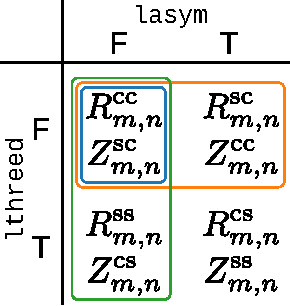
\includegraphics{img/4_term_DFT_coeffs.pdf}
  \caption{Coefficients to take into account for a given set of symmetry flags $\texttt{lasym}$ and $\texttt{lasym}$.
  The blue   box (top left corner) contains the coefficients required for  symmetric   two-dimensional configurations.
  The orange box (top row)         contains the coefficients required for asymmetric   two-dimensional configurations.
  The green  box (left column)     contains the coefficients required for  symmetric three-dimensional configurations.
  All coefficients                                       are required for asymmetric three-dimensional configurations.
  $R$ can be seen as a placeholder for all quantities with cosine parity.
  $Z$ can be seen as a placeholder for all quantities with   sine parity.}
  \label{fig:4_term_DFT_coeffs}
\end{figure}

The tangential derivatives of the state variables in VMEC are computed analytically
as laid out in Sec.~\ref{sec:tangential_derivatives}.
For the four-term separable-product Fourier basis described above,
the tangential derivatives are computed as follows.
The poloidal derivative $U(\theta,\zeta)$ of a state variable $X$ is given by:
\begin{align}
  U(\theta,\zeta) = \frac{\partial X}{\partial \theta} (\theta, \zeta)
  =&          \sum_{m=0}^M \sum_{n=0}^N \Biggl[    - m \hat{X}_{m,n}^\mathrm{cc} \sin(m \theta) \cos(n \zeta)
                                                   + m \hat{X}_{m,n}^\mathrm{ss} \cos(m \theta) \sin(n \zeta) \nonumber \\
  ~& \phantom{\sum_{m=0}^M \sum_{n=0}^N \Biggl[}\, + m \hat{X}_{m,n}^\mathrm{sc} \cos(m \theta) \cos(n \zeta)
                                                   - m \hat{X}_{m,n}^\mathrm{cs} \sin(m \theta) \sin(n \zeta) \Biggr]
\end{align}
which can be reformulated as
\begin{align}
  U(\theta,\zeta)
  =&          \sum_{m=0}^M \sum_{n=0}^N \Biggl[    \phantom{+}\, \hat{U}_{m,n}^\mathrm{cc} \cos(m \theta) \cos(n \zeta)
                                                            +    \hat{U}_{m,n}^\mathrm{ss} \sin(m \theta) \sin(n \zeta) \nonumber \\
  ~& \phantom{\sum_{m=0}^M \sum_{n=0}^N \Biggl[}\,          +    \hat{U}_{m,n}^\mathrm{sc} \sin(m \theta) \cos(n \zeta)
                                                            +    \hat{U}_{m,n}^\mathrm{cs} \cos(m \theta) \sin(n \zeta) \Biggr]
\end{align}
with
\begin{align}
  \hat{U}_{m,n}^\mathrm{cc} &= + m \hat{X}_{m,n}^\mathrm{sc} \\
  \hat{U}_{m,n}^\mathrm{ss} &= - m \hat{X}_{m,n}^\mathrm{cs} \\
  \hat{U}_{m,n}^\mathrm{sc} &= - m \hat{X}_{m,n}^\mathrm{cc} \\
  \hat{U}_{m,n}^\mathrm{cs} &= + m \hat{X}_{m,n}^\mathrm{ss} \, .
\end{align}
The toroidal derivative $V(\theta,\zeta)$ of a state variable $X$ is given by:
\begin{align}
  ~&\, V(\theta,\zeta) = \frac{\partial X}{\partial \phi} \underbrace{\frac{\partial \phi}{\partial \zeta}}_{= n_\mathrm{fp}} (\theta, \zeta) \nonumber \\
  =&\,          \sum_{m=0}^M \sum_{n=0}^N \Biggl[    - n n_\mathrm{fp} \hat{X}_{m,n}^\mathrm{cc} \cos(m \theta) \sin(n \zeta)
                                                     + n n_\mathrm{fp} \hat{X}_{m,n}^\mathrm{ss} \sin(m \theta) \cos(n \zeta) \nonumber \\
  ~&\, \phantom{\sum_{m=0}^M \sum_{n=0}^N \Biggl[}\, - n n_\mathrm{fp} \hat{X}_{m,n}^\mathrm{sc} \sin(m \theta) \sin(n \zeta)
                                                     + n n_\mathrm{fp} \hat{X}_{m,n}^\mathrm{cs} \cos(m \theta) \cos(n \zeta) \Biggr]
\end{align}
which can be reformulated as
\begin{align}
  V(\theta,\zeta)
  =&          \sum_{m=0}^M \sum_{n=0}^N \Biggl[    \phantom{+}\, \hat{V}_{m,n}^\mathrm{cc} \cos(m \theta) \cos(n \zeta)
                                                            +    \hat{V}_{m,n}^\mathrm{ss} \sin(m \theta) \sin(n \zeta) \nonumber \\
  ~& \phantom{\sum_{m=0}^M \sum_{n=0}^N \Biggl[}\,          +    \hat{V}_{m,n}^\mathrm{sc} \sin(m \theta) \cos(n \zeta)
                                                            +    \hat{V}_{m,n}^\mathrm{cs} \cos(m \theta) \sin(n \zeta) \Biggr]
\end{align}
with
\begin{align}
  \hat{V}_{m,n}^\mathrm{cc} &= + n n_\mathrm{fp} \hat{X}_{m,n}^\mathrm{cs} \\
  \hat{V}_{m,n}^\mathrm{ss} &= - n n_\mathrm{fp} \hat{X}_{m,n}^\mathrm{sc} \\
  \hat{V}_{m,n}^\mathrm{sc} &= + n n_\mathrm{fp} \hat{X}_{m,n}^\mathrm{ss} \\
  \hat{V}_{m,n}^\mathrm{cs} &= - n n_\mathrm{fp} \hat{X}_{m,n}^\mathrm{cc} \, .
\end{align}
The symmetry properties of the tangential derivatives are shown in Fig.~\ref{fig:4_term_DFT_derivatives}.
\begin{figure}[h]
  \centering
  \begin{minipage}[b]{0.49\textwidth}
    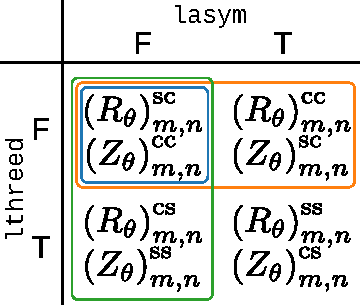
\includegraphics{img/4_term_DFT_dTheta.pdf}
  \end{minipage}
  \hfill
  \begin{minipage}[b]{0.49\textwidth}
    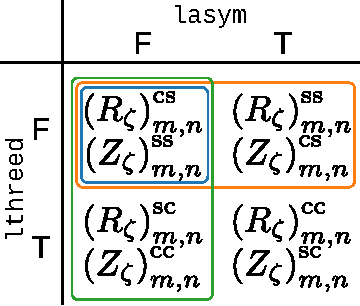
\includegraphics{img/4_term_DFT_dZeta.pdf}
  \end{minipage}
  \caption{Coefficients to take into account for a given set of symmetry flags $\texttt{lasym}$ and $\texttt{lasym}$
  when evaluating the tangential derivatives in poloidal (left panel) and toroidal (right panel) directions.
  The blue   box (top left corner) contains the coefficients required for  symmetric   two-dimensional configurations.
  The orange box (top row)         contains the coefficients required for asymmetric   two-dimensional configurations.
  The green  box (left column)     contains the coefficients required for  symmetric three-dimensional configurations.
  All coefficients                                       are required for asymmetric three-dimensional configurations.}
  \label{fig:4_term_DFT_derivatives}
\end{figure}
Above inverse Fourier transforms are evaluated in the symmetric case only on half of the poloidal interval.
This gives the real-space representation of the quantities, which due to the definite-parity basis functions then also have a definite parity.
This is implemented in the Fortran implementation of VMEC in the subroutine~\texttt{totzsps}.
In the asymmetric case, the same routine is used to compute the contribution to the quantities
with that parity those quantities would have in the symmetric case.
Additionally, a second routine is used to compute the other-parity contributions to the quantities,
also only on half the poloidal interval. This is done in~\texttt{totzspa}.
These contributions are combined in the asymmetric case to yield the asymmetric quantites on the full interval.
This is a two-step process and it is implemented in~\texttt{symrzl}.
First, the ``extended'' interval~$]\pi,2\pi[$ needs to be filled,
since the original data (present in $[0,\pi]$) must not be overwritten.
Then, the first half of the interval ($[0,\pi]$) is overwritten in-place
with the combination of the symmetric and anti-symmetric contributions.

\begin{figure}[htbp]
  \centering
  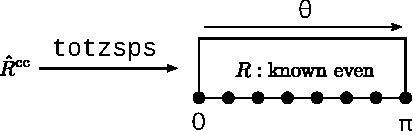
\includegraphics{img/R_sym.pdf}
  \caption{The real-space $R$~coordinate is known to have even parity in the symmetric case.
  It is computed from the Fourier coefficients~$\hat{R}^\mathrm{cc}$.}
  \label{fig:R_sym}
\end{figure}

\begin{figure}[htbp]
  \centering
  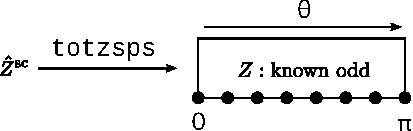
\includegraphics{img/Z_sym.pdf}
  \caption{The real-space $Z$~coordinate is known to have odd parity in the symmetric case.
  It is computed from the Fourier coefficients~$\hat{Z}^\mathrm{sc}$.}
  \label{fig:Z_sym}
\end{figure}

\begin{figure}[htbp]
  \centering
  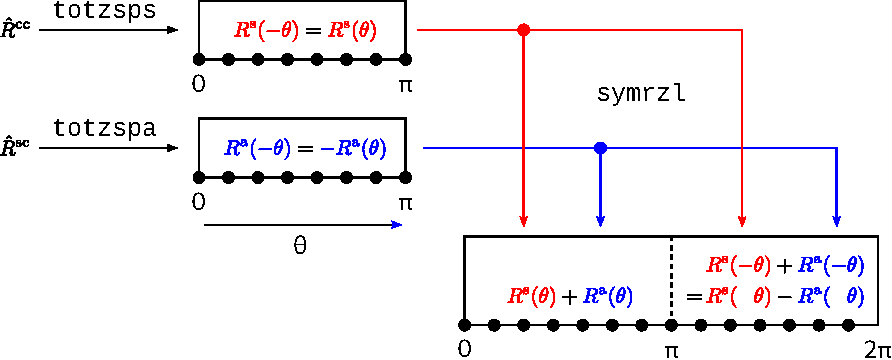
\includegraphics{img/R_asym.pdf}
  \caption{The real-space $R$~coordinate is constructed from its even-parity and odd-parity components in the general case.
  The even-parity component is the even~$R$ of the symmetric case, computed from the Fourier coefficients~$\hat{R}^\mathrm{cc}$.
  The  odd-parity component is computed additionally in the asymmetric case from the Fourier coefficients~$\hat{R}^\mathrm{sc}$.
  These components are combined using \texttt{symrzl} to yield the general~$R$ on the full poloidal domain.}
  \label{fig:R_asym}
\end{figure}

\begin{figure}[htbp]
  \centering
  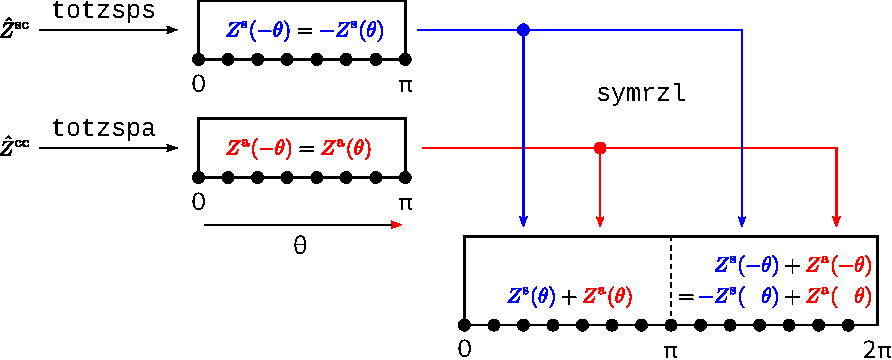
\includegraphics{img/Z_asym.pdf}
  \caption{The real-space $Z$~coordinate is constructed from its even-parity and odd-parity components in the general case.
  The  odd-parity component is the odd~$Z$ of the symmetric case, computed from the Fourier coefficients~$\hat{Z}^\mathrm{sc}$.
  The even-parity component is computed additionally in the asymmetric case from the Fourier coefficients~$\hat{Z}^\mathrm{cc}$.
  These components are combined using \texttt{symrzl} to yield the general~$Z$ on the full poloidal domain.}
  \label{fig:Z_asym}
\end{figure}

\FloatBarrier
\section{Jacobian} \label{sec:jacobian}
The Jacobian $\sqrt{g}$ is computed on the radial half-grid.
The Jacobian is decomposed into a toroidal factor $R$
and the two-dimensional Jacobian in the poloidal plane $\tau$:
\begin{align}
                  \sqrt{g} =&\, R \tau \\
  \textrm{with} \quad \tau =&\, R_\theta Z_s - R_s Z_\theta \, .
\end{align}
This is Eqn.~(17) with $\tau = G$ in Ref.~\cite{hirshman_whitson_1983}.
The terms appearing in above expression must be combined from contributions due to even-$m$ and odd-$m$ Fourier harmonics~\cite{hirshman_schwenn_nuehrenberg_1990}:
\begin{equation}
  X(s) = X^\mathrm{e}(s) + \sqrt{s} X^\mathrm{o}(s) \label{eqn:even_odd_comb}
\end{equation}
for $X \in \{ R, Z, R_\theta, Z_\theta, ... \}$.
The geometry of the flux surfaces $R$, $Z$ and its tangential derivatives are available on the full grid.
The geometry and the tangential derivatives are interpolated/averaged onto intermediate half-grid points.
Radial derivatives are computed using finite differences over neighboring full-grid points.
This leads to the following for $R$ and for the tangential derivatives:
\begin{align}
  R(s_{j-\half})        =&\, \frac{1}{2} \left[ R(s_j) + R(s_{j-1}) \right] \\
                        =&\, \frac{1}{2} \left[                      \left( R^\mathrm{e}(s_j) + R^\mathrm{e}(s_{j-1}) \right)
                                                + \sqrt{s_{j-\half}} \left( R^\mathrm{o}(s_j) + R^\mathrm{o}(s_{j-1}) \right) \right] \label{eqn:r_half} \\
  R_\theta(s_{j-\half}) =&\, \frac{1}{2} \left[ R_\theta(s_j) + R_\theta(s_{j-1}) \right] \\
                        =&\, \frac{1}{2} \left[                      \left( R_\theta^\mathrm{e}(s_j) + R_\theta^\mathrm{e}(s_{j-1}) \right)
                                                + \sqrt{s_{j-\half}} \left( R_\theta^\mathrm{o}(s_j) + R_\theta^\mathrm{o}(s_{j-1}) \right) \right] \\
  Z_\theta(s_{j-\half}) =&\, \frac{1}{2} \left[ Z_\theta(s_j) + Z_\theta(s_{j-1}) \right] \\
                        =&\, \frac{1}{2} \left[                      \left( Z_\theta^\mathrm{e}(s_j) + Z_\theta^\mathrm{e}(s_{j-1}) \right)
                                                + \sqrt{s_{j-\half}} \left( Z_\theta^\mathrm{o}(s_j) + Z_\theta^\mathrm{o}(s_{j-1}) \right) \right] \, .
\end{align}
The chain rule needs to be taken into account when computing the radial derivatives (see Sec.~\ref{sec:radial_discretization}).
The radial derivatives can be decomposed into two parts:
\begin{align}
  R_s(s_{j-\half}) =&\, {\tilde{R_s}}(s_{j-\half}) + \frac{1}{2 \sqrt{s_{j-\half}}} R^\mathrm{o}(s_{j-\half}) \\
  Z_s(s_{j-\half}) =&\, {\tilde{Z_s}}(s_{j-\half}) + \frac{1}{2 \sqrt{s_{j-\half}}} Z^\mathrm{o}(s_{j-\half}) \, .
\end{align}
The first terms in above expression are computed using finite differences as follows:
\begin{align}
  {\tilde{R_s}}(s_{j-\half}) =&\, \frac{1}{\Delta s} \left[ R(s_j) - R(s_{j-1}) \right] \\
                             =&\, \frac{1}{\Delta s} \left[                      \left( R^\mathrm{e}(s_j) - R^\mathrm{e}(s_{j-1}) \right)
                                                            + \sqrt{s_{j-\half}} \left( R^\mathrm{o}(s_j) - R^\mathrm{o}(s_{j-1}) \right) \right] \\
  {\tilde{Z_s}}(s_{j-\half}) =&\, \frac{1}{\Delta s} \left[ Z(s_j) - Z(s_{j-1}) \right] \\
                             =&\, \frac{1}{\Delta s} \left[                      \left( Z^\mathrm{e}(s_j) - Z^\mathrm{e}(s_{j-1}) \right)
                                                            + \sqrt{s_{j-\half}} \left( Z^\mathrm{o}(s_j) - Z^\mathrm{o}(s_{j-1}) \right) \right] \, .
\end{align}
Inserting the radial derivatives into the expression for $\tau$, we arrive at:
\begin{align}
  \tau(s_{j-\half}) =&\, \phantom{-}\, R_\theta(s_{j-\half}) \left[ {\tilde{Z_s}}(s_{j-\half}) + \frac{1}{2 \sqrt{s_{j-\half}}} Z^\mathrm{o}(s_{j-\half}) \right] \nonumber \\
                    ~&\,          -    \left[ {\tilde{R_s}}(s_{j-\half}) + \frac{1}{2 \sqrt{s_{j-\half}}} R^\mathrm{o}(s_{j-\half}) \right] Z_\theta(s_{j-\half}) \nonumber \\
                    =&\,   R_\theta(s_{j-\half}) {\tilde{Z_s}}(s_{j-\half}) - {\tilde{R_s}}(s_{j-\half}) Z_\theta(s_{j-\half}) \nonumber \\
                    ~&\, + \frac{1}{2 \sqrt{s_{j-\half}}} \left[ R_\theta(s_{j-\half}) Z^\mathrm{o}(s_{j-\half}) - R^\mathrm{o}(s_{j-\half}) Z_\theta(s_{j-\half}) \right] \label{eqn:tau_almost}
\end{align}
The last term has to be expanded further:
\begin{align}
   R_\theta(s_{j-\half}) Z^\mathrm{o}(s_{j-\half})
  =&\, \left[ R_\theta^\mathrm{e}(s_{j-\half}) + \sqrt{s_{j-\half}} R_\theta^\mathrm{o}(s_{j-\half}) \right] Z^\mathrm{o}(s_{j-\half}) \nonumber \\
  =&\, R_\theta^\mathrm{e}(s_{j-\half}) Z^\mathrm{o}(s_{j-\half}) + \sqrt{s_{j-\half}} R_\theta^\mathrm{o}(s_{j-\half}) Z^\mathrm{o}(s_{j-\half}) \\
   R^\mathrm{o}(s_{j-\half}) Z_\theta(s_{j-\half})
  =&\, R^\mathrm{o}(s_{j-\half}) \left[ Z_\theta^\mathrm{e}(s_{j-\half}) + \sqrt{s_{j-\half}} Z_\theta^\mathrm{o}(s_{j-\half}) \right] \nonumber \\
  =&\, R^\mathrm{o}(s_{j-\half}) Z_\theta^\mathrm{e}(s_{j-\half}) + \sqrt{s_{j-\half}} R^\mathrm{o}(s_{j-\half}) Z_\theta^\mathrm{o}(s_{j-\half})
\end{align}
Inserting this into the expression for $\tau$ from \eqn{tau_almost} leads to:
\begin{align}
  \tau(s_{j-\half}) =&\,   R_\theta(s_{j-\half}) {\tilde{Z_s}}(s_{j-\half}) - {\tilde{R_s}}(s_{j-\half}) Z_\theta(s_{j-\half}) \nonumber \\
                    ~&\, + \frac{1}{2 \sqrt{s_{j-\half}}} \Bigl\{
                      \phantom{-}\,  R_\theta^\mathrm{e}(s_{j-\half}) Z^\mathrm{o}(s_{j-\half}) + \sqrt{s_{j-\half}} R_\theta^\mathrm{o}(s_{j-\half}) Z^\mathrm{o}(s_{j-\half}) \nonumber \\
                    ~&\, \phantom{+    \frac{1}{2 \sqrt{s_{j-\half}}} \Bigl\{}\,
                               - R^\mathrm{o}(s_{j-\half}) Z_\theta^\mathrm{e}(s_{j-\half}) - \sqrt{s_{j-\half}} R^\mathrm{o}(s_{j-\half}) Z_\theta^\mathrm{o}(s_{j-\half}) \Bigr\} \nonumber \\
                    =&\,   R_\theta(s_{j-\half}) {\tilde{Z_s}}(s_{j-\half}) - {\tilde{R_s}}(s_{j-\half}) Z_\theta(s_{j-\half}) \nonumber \\
                    ~&\, + \frac{1}{2 \sqrt{s_{j-\half}}} \left[ R_\theta^\mathrm{e}(s_{j-\half}) Z^\mathrm{o}(s_{j-\half}) - R^\mathrm{o}(s_{j-\half}) Z_\theta^\mathrm{e}(s_{j-\half}) \right] \nonumber \\
                    ~&\, + \frac{1}{2}                    \left[ R_\theta^\mathrm{o}(s_{j-\half}) Z^\mathrm{o}(s_{j-\half}) - R^\mathrm{o}(s_{j-\half}) Z_\theta^\mathrm{o}(s_{j-\half}) \right]
\end{align}
Here, the product interpolation rule~\eqn{product_interp} has to be employed:
\begin{align}
  R_\theta^\mathrm{e}(s_{j-\half}) Z^\mathrm{o}(s_{j-\half}) =&\, \frac{1}{2} \Bigl[ R_\theta^\mathrm{e}(s_{j}) Z^\mathrm{o}(s_{j}) + R_\theta^\mathrm{e}(s_{j-1}) Z^\mathrm{o}(s_{j-1}) \Bigr] \\
  R^\mathrm{o}(s_{j-\half}) Z_\theta^\mathrm{e}(s_{j-\half}) =&\, \frac{1}{2} \Bigl[ R^\mathrm{o}(s_{j}) Z_\theta^\mathrm{e}(s_{j}) + R^\mathrm{o}(s_{j-1}) Z_\theta^\mathrm{e}(s_{j-1}) \Bigr] \\
  R_\theta^\mathrm{o}(s_{j-\half}) Z^\mathrm{o}(s_{j-\half}) =&\, \frac{1}{2} \Bigl[ R_\theta^\mathrm{o}(s_{j}) Z^\mathrm{o}(s_{j}) + R_\theta^\mathrm{o}(s_{j-1}) Z^\mathrm{o}(s_{j-1}) \Bigr] \\
  R^\mathrm{o}(s_{j-\half}) Z_\theta^\mathrm{o}(s_{j-\half}) =&\, \frac{1}{2} \Bigl[ R^\mathrm{o}(s_{j}) Z_\theta^\mathrm{o}(s_{j}) + R^\mathrm{o}(s_{j-1}) Z_\theta^\mathrm{o}(s_{j-1}) \Bigr] \, .
\end{align}
Finally, $\tau$ is assembled as follows:
\begin{align}
  \tau(s_{j-\half}) =&\,   R_\theta(s_{j-\half}) {\tilde{Z_s}}(s_{j-\half}) - {\tilde{R_s}}(s_{j-\half}) Z_\theta(s_{j-\half}) \nonumber \\
                    ~&\, + \frac{1}{4 \sqrt{s_{j-\half}}} \Bigl[ \phantom{-}\, R_\theta^\mathrm{e}(s_{j}) Z^\mathrm{o}(s_{j}) + R_\theta^\mathrm{e}(s_{j-1}) Z^\mathrm{o}(s_{j-1}) \nonumber \\
           ~&\, \phantom{+ \frac{1}{4 \sqrt{s_{j-\half}}} \Bigl[}\,       -    R^\mathrm{o}(s_{j}) Z_\theta^\mathrm{e}(s_{j}) - R^\mathrm{o}(s_{j-1}) Z_\theta^\mathrm{e}(s_{j-1}) \Bigr] \nonumber \\
                    ~&\, + \frac{1}{4}                    \Bigl[ \phantom{-}\, R_\theta^\mathrm{o}(s_{j}) Z^\mathrm{o}(s_{j}) + R_\theta^\mathrm{o}(s_{j-1}) Z^\mathrm{o}(s_{j-1}) \nonumber \\
           ~&\, \phantom{+ \frac{1}{4}                    \Bigl[}\,       -    R^\mathrm{o}(s_{j}) Z_\theta^\mathrm{o}(s_{j}) - R^\mathrm{o}(s_{j-1}) Z_\theta^\mathrm{o}(s_{j-1}) \Bigr] \label{eqn:tau_final}
\end{align}
The Jacobian on the half-grid can then be assembled without further due:
\begin{equation}
  \sqrt{g}(s_{j-\half}) = R(s_{j-\half}) \tau(s_{j-\half})
\end{equation}
with $R(s_{j-\half})$ from \eqn{r_half} and $\tau(s_{j-\half})$ from \eqn{tau_final}.

\FloatBarrier
\section{Metric Elements} \label{sec:metric_elements}
The metric elements $g_{\alpha \beta}$ with $(\alpha, \beta) \in \{ \theta, \zeta \}$ are given by:
\begin{equation}
  g_{\alpha \beta} = R_\alpha R_\beta + Z_\alpha Z_\beta + \delta_{\alpha \zeta} \delta_{\beta \zeta} R^2 \, . \label{eqn:metric_elements_abstract}
\end{equation}
Concretely, this leads to~\cite{geiger_calc_current_in_prout}:
\begin{align}
  g_{\theta \theta} =&\, \left( \frac{\partial R}{\partial \theta} \right)^2 + \left( \frac{\partial Z}{\partial \theta} \right)^2 \\
  g_{\theta \zeta } =&\, \frac{\partial R}{\partial \theta} \frac{\partial R}{\partial \zeta} + \frac{\partial Z}{\partial \theta} \frac{\partial Z}{\partial \zeta} \\
  g_{\zeta  \zeta } =&\, \left( \frac{\partial R}{\partial \zeta } \right)^2 + \left( \frac{\partial Z}{\partial \zeta } \right)^2 + R^2 \, .
\end{align}
The individual terms in above expressions are composed of contributions from even-$m$ and odd-$m$ Fourier harmonics as noted in~\eqn{even_odd_comb}.
Inserting this decomposition into the abstract metric element expression from~\eqn{metric_elements_abstract} leads to:
\begin{align}
  g_{\alpha \beta} =&\, \phantom{+}\, \left( R_\alpha^\mathrm{e} + \sqrt{s} R_\alpha^\mathrm{o} \right) \left( R_\beta^\mathrm{e} + \sqrt{s} R_\beta^\mathrm{o} \right) \nonumber \\
                   ~&\,          +    \left( Z_\alpha^\mathrm{e} + \sqrt{s} Z_\alpha^\mathrm{o} \right) \left( Z_\beta^\mathrm{e} + \sqrt{s} Z_\beta^\mathrm{o} \right) \nonumber \\
                   ~&\,          +    \delta_{\alpha \zeta} \delta_{\beta \zeta} \left( R^\mathrm{e} + \sqrt{s} R^\mathrm{o} \right) \left( R^\mathrm{e} + \sqrt{s} R^\mathrm{o} \right) \nonumber \\
                   =&\, \phantom{+ \sqrt{s}}~ \left(   R_\alpha^\mathrm{e} R_\beta^\mathrm{e} + Z_\alpha^\mathrm{e} Z_\beta^\mathrm{e}
                                                     + \delta_{\alpha \zeta} \delta_{\beta \zeta} R^\mathrm{e} R^\mathrm{e} \right) \nonumber \\
                   ~&\,          + \sqrt{s}   \left(   R_\alpha^\mathrm{e} R_\beta^\mathrm{o} + R_\alpha^\mathrm{o} R_\beta^\mathrm{e}
                                                     + Z_\alpha^\mathrm{e} Z_\beta^\mathrm{o} + Z_\alpha^\mathrm{o} Z_\beta^\mathrm{e}
                                                     + 2 \delta_{\alpha \zeta} \delta_{\beta \zeta} R^\mathrm{e} R^\mathrm{o} \right) \nonumber \\
                   ~&\,          + ~~s~       \left(   R_\alpha^\mathrm{o} R_\beta^\mathrm{o} + Z_\alpha^\mathrm{o} Z_\beta^\mathrm{o}
                                                     + \delta_{\alpha \zeta} \delta_{\beta \zeta} R^\mathrm{o} R^\mathrm{o} \right) \, . \label{eqn:metric_elements_evenodd}
\end{align}
Direct evaluation of this intermediate result at $s_{j-\half}$ leads to Eqn.~(10) in Ref.~\cite{hirshman_schwenn_nuehrenberg_1990}
(up to the omitted term $\delta_{\alpha \zeta} \delta_{\beta \zeta} R^2$):
\begin{align}
  g_{\alpha \beta}^{j-\half} =&\, \phantom{+ \sqrt{s_{j-\half}}}~ \left(   R_\alpha^\mathrm{e} R_\beta^\mathrm{e} + Z_\alpha^\mathrm{e} Z_\beta^\mathrm{e}
                                                                         + \delta_{\alpha \zeta} \delta_{\beta \zeta} R^\mathrm{e} R^\mathrm{e} \right)^{j-\half} \nonumber \\
                             ~&\,          + \sqrt{s_{j-\half}}   \left(   R_\alpha^\mathrm{e} R_\beta^\mathrm{o} + R_\alpha^\mathrm{o} R_\beta^\mathrm{e}
                                                                         + Z_\alpha^\mathrm{e} Z_\beta^\mathrm{o} + Z_\alpha^\mathrm{o} Z_\beta^\mathrm{e}
                                                                         + 2 \delta_{\alpha \zeta} \delta_{\beta \zeta} R^\mathrm{e} R^\mathrm{o} \right)^{j-\half} \nonumber \\
                             ~&\,          + ~~s_{j-\half}~       \left(   R_\alpha^\mathrm{o} R_\beta^\mathrm{o} + Z_\alpha^\mathrm{o} Z_\beta^\mathrm{o}
                                                                         + \delta_{\alpha \zeta} \delta_{\beta \zeta} R^\mathrm{o} R^\mathrm{o} \right)^{j-\half} \, . \label{eqn:metric_elements_10}
\end{align}
What is implemented in VMEC is different.
It suggests the following interpretation.
Suppose the metric elements $g_{\alpha \beta}$ can also be decomposed into even-$m$ and odd-$m$ contributions:
\begin{equation}
  g_{\alpha \beta} = g_{\alpha \beta}^\mathrm{e} + \sqrt{s} \, g_{\alpha \beta}^\mathrm{o} \, .
\end{equation}
Then, interpolation onto the half-grid would be done separately:
\begin{equation}
  g_{\alpha \beta}^{j-\half} = g_{\alpha \beta}^{\mathrm{e}, j-\half} + \sqrt{s_{j-\half}} \, g_{\alpha \beta}^{\mathrm{o}, j-\half} \, .
\end{equation}
The odd-$m$ contributions to the metric elements are odd functions of the poloidal coordinate.
Thus, the radial regularization factors~$ \sqrt{s}$ need to be factored out prior to interpolation onto the half-grid.
However, in the metric elements, products of two odd-$m$-terms appear (see, e.g., the last group in \eqn{metric_elements_evenodd}).
The product of two odd functions is an even function again.
The interpolation of this function onto the half-grid therefore should happen without factoring out the $\sqrt{s}$ normalization factors.
However, all odd-$m$ terms in the current VMEC implementation have them factored in already.
Therefore, one needs to cancel the factor $s = \sqrt{s} \sqrt{s}$ (where each $\sqrt{s}$ stems from one of the odd-$m$ factors)
before performing the radial interpolation onto the half-grid.
Concretely, this leads to:
\begin{align}
  g_{\alpha \beta}^{j-\half} =&\, \left[     \left(   R_\alpha^\mathrm{e} R_\beta^\mathrm{e} + Z_\alpha^\mathrm{e} Z_\beta^\mathrm{e}
                                                    + \delta_{\alpha \zeta} \delta_{\beta \zeta} R^\mathrm{e} R^\mathrm{e} \right)
                                         + s \left(   R_\alpha^\mathrm{o} R_\beta^\mathrm{o} + Z_\alpha^\mathrm{o} Z_\beta^\mathrm{o}
                                                    + \delta_{\alpha \zeta} \delta_{\beta \zeta} R^\mathrm{o} R^\mathrm{o} \right) \right]^{j-\half} \nonumber \\
                             ~&\, + \sqrt{s_{j-\half}}   \left(   R_\alpha^\mathrm{e} R_\beta^\mathrm{o} + R_\alpha^\mathrm{o} R_\beta^\mathrm{e}
                                                                + Z_\alpha^\mathrm{e} Z_\beta^\mathrm{o} + Z_\alpha^\mathrm{o} Z_\beta^\mathrm{e}
                                                                + 2 \delta_{\alpha \zeta} \delta_{\beta \zeta} R^\mathrm{e} R^\mathrm{o} \right)^{j-\half} \, .
\end{align}
Application of the product interpolation rule~\eqn{product_interp} leads to:
\begin{align}
  g_{\alpha \beta}^{j-\half} =&\,          \frac{1}{2} \Biggl[    \phantom{+ s_{j-1}}~  \left(   R_\alpha^\mathrm{e} R_\beta^\mathrm{e} + Z_\alpha^\mathrm{e} Z_\beta^\mathrm{e}
                                                                                               + \delta_{\alpha \zeta} \delta_{\beta \zeta} R^\mathrm{e} R^\mathrm{e} \right)^j     \nonumber \\
                             ~&\, \phantom{\frac{1}{2} \Biggl[}\, + \phantom{s_{j-1}}   \left(   R_\alpha^\mathrm{e} R_\beta^\mathrm{e} + Z_\alpha^\mathrm{e} Z_\beta^\mathrm{e}
                                                                                               + \delta_{\alpha \zeta} \delta_{\beta \zeta} R^\mathrm{e} R^\mathrm{e} \right)^{j-1} \nonumber \\
                             ~&\, \phantom{\frac{1}{2} \Biggl[}\, +          s_j ~~\,   \left(   R_\alpha^\mathrm{o} R_\beta^\mathrm{o} + Z_\alpha^\mathrm{o} Z_\beta^\mathrm{o}
                                                                                               + \delta_{\alpha \zeta} \delta_{\beta \zeta} R^\mathrm{o} R^\mathrm{o} \right)^j     \nonumber \\
                             ~&\, \phantom{\frac{1}{2} \Biggl[}\, +          s_{j-1}    \left(   R_\alpha^\mathrm{o} R_\beta^\mathrm{o} + Z_\alpha^\mathrm{o} Z_\beta^\mathrm{o}
                                                                                               + \delta_{\alpha \zeta} \delta_{\beta \zeta} R^\mathrm{o} R^\mathrm{o} \right)^{j-1} \Biggr] \nonumber \\
                             ~&\,          + \frac{1}{2} \sqrt{s_{j-\half}} \Biggl[ \phantom{+}\, \left(   R_\alpha^\mathrm{e} R_\beta^\mathrm{o} + R_\alpha^\mathrm{o} R_\beta^\mathrm{e}
                                                                                                         + Z_\alpha^\mathrm{e} Z_\beta^\mathrm{o} + Z_\alpha^\mathrm{o} Z_\beta^\mathrm{e}
                                                                                                         + 2 \delta_{\alpha \zeta} \delta_{\beta \zeta} R^\mathrm{e} R^\mathrm{o} \right)^j \nonumber \\
                             ~&\, \phantom{+ \frac{1}{2} \sqrt{s_{j-\half}} \Biggl[}\,       +    \left(   R_\alpha^\mathrm{e} R_\beta^\mathrm{o} + R_\alpha^\mathrm{o} R_\beta^\mathrm{e}
                                                                                                         + Z_\alpha^\mathrm{e} Z_\beta^\mathrm{o} + Z_\alpha^\mathrm{o} Z_\beta^\mathrm{e}
                                                                                                         + 2 \delta_{\alpha \zeta} \delta_{\beta \zeta} R^\mathrm{e} R^\mathrm{o} \right)^{j-1} \Biggr]
\end{align}
Concretely:
\begin{align}
  g_{\theta \theta}^{j-\half} =&\, \phantom{+}~ \frac{1}{2} \left[           \left( R_\theta^\mathrm{e} R_\theta^\mathrm{e} + Z_\theta^\mathrm{e} Z_\theta^\mathrm{e} \right)^j
                                                                   +         \left( R_\theta^\mathrm{e} R_\theta^\mathrm{e} + Z_\theta^\mathrm{e} Z_\theta^\mathrm{e} \right)^{j-1} \right] \nonumber \\
                              ~&\,          +   \frac{1}{2} \left[   s_j     \left( R_\theta^\mathrm{o} R_\theta^\mathrm{o} + Z_\theta^\mathrm{o} Z_\theta^\mathrm{o} \right)^j
                                                                   + s_{j-1} \left( R_\theta^\mathrm{o} R_\theta^\mathrm{o} + Z_\theta^\mathrm{o} Z_\theta^\mathrm{o} \right)^{j-1} \right] \nonumber \\
                              ~&\,          + \sqrt{s_{j-\half}} \left[   \left( R_\theta^\mathrm{e} R_\theta^\mathrm{o} + Z_\theta^\mathrm{e} Z_\theta^\mathrm{o} \right)^j
                                                                        + \left( R_\theta^\mathrm{e} R_\theta^\mathrm{o} + Z_\theta^\mathrm{e} Z_\theta^\mathrm{o} \right)^{j-1} \right] \label{eqn:g_theta_theta} \\
  g_{\theta \zeta }^{j-\half} =&\, \phantom{+}~ \frac{1}{2} \left[           \left( R_\theta^\mathrm{e} R_\zeta^\mathrm{e} + Z_\theta^\mathrm{e} Z_\zeta^\mathrm{e} \right)^j
                                                                   +         \left( R_\theta^\mathrm{e} R_\zeta^\mathrm{e} + Z_\theta^\mathrm{e} Z_\zeta^\mathrm{e} \right)^{j-1} \right] \nonumber \\
                              ~&\,          +   \frac{1}{2} \left[   s_j     \left( R_\theta^\mathrm{o} R_\zeta^\mathrm{o} + Z_\theta^\mathrm{o} Z_\zeta^\mathrm{o} \right)^j
                                                                   + s_{j-1} \left( R_\theta^\mathrm{o} R_\zeta^\mathrm{o} + Z_\theta^\mathrm{o} Z_\zeta^\mathrm{o} \right)^{j-1} \right] \nonumber \\
                              ~&\, + \frac{1}{2} \sqrt{s_{j-\half}} \Bigl[ \phantom{+}\, \left(   R_\theta^\mathrm{e} R_\zeta^\mathrm{o} + R_\theta^\mathrm{o} R_\zeta^\mathrm{e}
                                                                                                + Z_\theta^\mathrm{e} Z_\zeta^\mathrm{o} + Z_\theta^\mathrm{o} Z_\zeta^\mathrm{e} \right)^j \nonumber \\
                              ~&\, \phantom{+ \frac{1}{2} \sqrt{s_{j-\half}} \Bigl[}\, + \left(   R_\theta^\mathrm{e} R_\zeta^\mathrm{o} + R_\theta^\mathrm{o} R_\zeta^\mathrm{e}
                                                                                                + Z_\theta^\mathrm{e} Z_\zeta^\mathrm{o} + Z_\theta^\mathrm{o} Z_\zeta^\mathrm{e} \right)^{j-1} \Bigr] \label{eqn:g_theta_zeta} \\
  g_{\zeta  \zeta }^{j-\half} =&\, \phantom{+}~ \frac{1}{2} \left[           \left( R_\zeta^\mathrm{e} R_\zeta^\mathrm{e} + Z_\zeta^\mathrm{e} Z_\zeta^\mathrm{e} + R^\mathrm{e} R^\mathrm{e} \right)^j
                                                                   +         \left( R_\zeta^\mathrm{e} R_\zeta^\mathrm{e} + Z_\zeta^\mathrm{e} Z_\zeta^\mathrm{e} + R^\mathrm{e} R^\mathrm{e} \right)^{j-1} \right] \nonumber \\
                              ~&\,          +   \frac{1}{2} \left[   s_j     \left( R_\zeta^\mathrm{o} R_\zeta^\mathrm{o} + Z_\zeta^\mathrm{o} Z_\zeta^\mathrm{o} + R^\mathrm{o} R^\mathrm{o} \right)^j
                                                                   + s_{j-1} \left( R_\zeta^\mathrm{o} R_\zeta^\mathrm{o} + Z_\zeta^\mathrm{o} Z_\zeta^\mathrm{o} + R^\mathrm{o} R^\mathrm{o} \right)^{j-1} \right] \nonumber \\
                              ~&\,          + \sqrt{s_{j-\half}} \left[   \left( R_\zeta^\mathrm{e} R_\zeta^\mathrm{o} + Z_\zeta^\mathrm{e} Z_\zeta^\mathrm{o} + R^\mathrm{e} R^\mathrm{o} \right)^j
                                                                        + \left( R_\zeta^\mathrm{e} R_\zeta^\mathrm{o} + Z_\zeta^\mathrm{e} Z_\zeta^\mathrm{o} + R^\mathrm{e} R^\mathrm{o} \right)^{j-1} \right] \, . \label{eqn:g_zeta_zeta}
\end{align}
This is what is actually implemented in VMEC.
A change to the variant in~\eqn{metric_elements_10} was tried,
but VMEC does not converge as fast as with the metric elements computed from~\eqn{g_theta_theta} to~\eqn{g_zeta_zeta}.

\FloatBarrier
\section{Constraint of Toroidal Current Profile}
The net toroidal current density is given by~\cite{hirshman_hogan_1986}:
\begin{equation}
  \langle j_\zeta \rangle = \int\limits_0^{2 \pi} \int\limits_0^{2 \pi} \underbrace{\left( \mathbf{j} \cdot \nabla \zeta \right)}_{=j_\zeta} \sqrt{g} \,\mathrm{d}\theta \,\mathrm{d}\zeta
                          = \frac{1}{(2 \pi)^2} \frac{\partial \langle B_\theta \rangle}{\partial s}
\end{equation}
with
\begin{equation}
  \langle B_\theta \rangle = \frac{1}{(2 \pi)^2} \int\limits_0^{2 \pi} \int\limits_0^{2 \pi} B_\theta \,\mathrm{d}\theta \,\mathrm{d}\zeta \, . \label{eqn:bsubu_bar}
\end{equation}
The net toroidal current enclosed by a given flux surface is $I_\zeta(s)$ with:
\begin{equation}
  \frac{\mu_0}{2 \pi} I_\zeta = \langle B_\theta \rangle \, . \label{eqn:curtor_bsubtheta}
\end{equation}
\eqn{bsubu_bar} is now inserted into \eqn{curtor_bsubtheta}:
\begin{equation}
  \frac{\mu_0}{2 \pi} I_\zeta = \frac{1}{(2 \pi)^2} \iint B_\theta \,\mathrm{d}\theta \,\mathrm{d}\zeta \, .
\end{equation}
The covariant magnetic field component $B_\theta$ is expressed using~\eqn{bsubtheta_from_contra}:
\begin{equation}
  \frac{\mu_0}{2 \pi} I_\zeta
  =
  \frac{1}{(2 \pi)^2} \iint \left( B^\theta g_{\theta \theta} + B^\zeta g_{\theta \zeta } \right) \,\mathrm{d}\theta \,\mathrm{d}\zeta \, . \label{eqn:constr_current_start}
\end{equation}
Inserting the explicit forms of the contravariant magnetic field components from~\eqn{bsuptheta} and~\eqn{bsupzeta},
it follows with~\eqn{constr_current_start}:
\begin{equation}
  \frac{\mu_0}{2 \pi} I_\zeta
  =
  \frac{1}{(2 \pi)^2}
  \iint \left[  \frac{  1  }{\sqrt{g}} \left( \chi' - \Phi' \lambda_\zeta  \right) g_{\theta \theta}
              + \frac{\Phi'}{\sqrt{g}} \left(   1   +       \lambda_\theta \right) g_{\theta \zeta } \right] \,\mathrm{d}\theta \,\mathrm{d}\zeta \, . \label{eqn:izeta_constraint}
\end{equation}
In \eqn{izeta_constraint}, $I_\zeta$, $\Phi'$, $\lambda$ and the geometric quantities $g_{\theta \theta}$, $g_{\theta \zeta}$ and $\sqrt{g}$ are given.
Thus, it is rearranged to yield the $\chi'$ profile compatible with the prescribed current profile:
\begin{align}
 \chi' \frac{1}{(2 \pi)^2} \iint \frac{g_{\theta \theta}}{\sqrt{g}} \,\mathrm{d}\theta \,\mathrm{d}\zeta
  =&\,
   \frac{\mu_0}{2 \pi} I_\zeta
 - \frac{1}{(2 \pi)^2}
   \iint \left[  \left(    - \frac{\Phi' \lambda_\zeta  }{\sqrt{g}} \right) g_{\theta \theta}
               + \left( \frac{\Phi' (1 + \lambda_\theta)}{\sqrt{g}} \right) g_{\theta \zeta } \right] \,\mathrm{d}\theta \,\mathrm{d}\zeta \\
\Leftrightarrow
 \chi'
  =&\,
  \frac{\frac{\mu_0}{2 \pi} I_\zeta - \frac{1}{(2 \pi)^2} \iint \left[  \left(    - \frac{\Phi' \lambda_\zeta  }{\sqrt{g}} \right) g_{\theta \theta}
                                                                      + \left( \frac{\Phi' (1 + \lambda_\theta)}{\sqrt{g}} \right) g_{\theta \zeta } \right] \,\mathrm{d}\theta \,\mathrm{d}\zeta}
       {\frac{1}{(2 \pi)^2} \iint \frac{g_{\theta \theta}}{\sqrt{g}} \,\mathrm{d}\theta \,\mathrm{d}\zeta} \, . \label{eqn:chip_from_current_constraint}
\end{align}
The rotational transform profile is then computed via:
\begin{equation}
 \iota = \frac{\chi'}{\Phi'} \, . \label{eqn:iota_from_fluxes}
\end{equation}
Eqn.~(11) in Ref.~\cite{hirshman_hogan_1986} is recovered for $I_\zeta = 0$, where above approach is termed the ``Zero-Current Algorithm''.
In VMEC, \eqn{chip_from_current_constraint} and \eqn{iota_from_fluxes} are evaluated at each time step and on every flux surface
to obtain the $\iota$ profile consistent with a prescribed net toroidal current profile.

In VMEC, $\lambda$ is one of the state variables that (together with the radial profiles and a few constants) completely define the MHD equilibrium.
In the following, the program flow is described that starts from $\lambda$ and the metric elements and results in the $\iota$ profile
consistent with the prescribed net toroidal current profile.
The factor $\Phi'$ is included in the $\lambda$ state variable since version~8.47 of VMEC.
It is normalized to the root-mean-square (RMS) value of the toroidal flux derivative (\texttt{lamscale}, see \eqn{lamscale}).
This was necessary for application of VMEC to RFPs, according to the release notes.
The tangential derivatives of $\lambda$ are computed first on the full-grid via an inverse DFT.
Contributions from even-$m$ and odd-$m$ Fourier harmonics are kept separately.
The normalization factor $\lambda_\textrm{scale} (= \code{lamscale})$ is multiplied in again
to retrieve the physically relevant quantities:
\begin{align}
  \code{lu}^\mathrm{e} \leftarrow&\, \lambda_\textrm{scale}             \left[\phantom{-} \frac{\Phi'}{\lambda_\textrm{scale}} \left( \frac{\partial \lambda}{\partial \theta} \right)^\mathrm{e} \right] \\
  \code{lu}^\mathrm{o} \leftarrow&\, \lambda_\textrm{scale}             \left[\phantom{-} \frac{\Phi'}{\lambda_\textrm{scale}} \left( \frac{\partial \lambda}{\partial \theta} \right)^\mathrm{o} \right] \\
  \code{lv}^\mathrm{e} \leftarrow&\, \lambda_\textrm{scale}             \left[         -  \frac{\Phi'}{\lambda_\textrm{scale}} \left( \frac{\partial \lambda}{\partial \zeta } \right)^\mathrm{e} \right] \\
  \code{lv}^\mathrm{o} \leftarrow&\, \lambda_\textrm{scale} \underbrace{\left[         -  \frac{\Phi'}{\lambda_\textrm{scale}} \left( \frac{\partial \lambda}{\partial \zeta } \right)^\mathrm{o} \right]}_{\textrm{from inv-DFTs}} \, .
\end{align}
In the next step, $\Phi'$ is added to $\code{lu}^\mathrm{e}$ in order to arrive at:
\begin{equation}
 \code{lu}^\mathrm{e} \leftarrow \code{lu}^\mathrm{e} + \Phi' = \Phi' \left( 1 + \left(\frac{\partial \lambda}{\partial \theta} \right)^\mathrm{e} \right) \, . \label{eqn:lu_e_full}
\end{equation}
All of this is still on the full-grid.
The offset~(= $(m=0)$ - contribution) of $1$ is only present in the even-$m$ term of \code{lu}, since the $(m=0)$ - contribution has even parity.
Above computations happen on the full-grid.
It is now required to interpolate these contributions onto the half-grid
in order to compute the contravariant magnetic field components,
where also the Jacobian and radial derivatives (later required for the MHD forces) are available.
Additionally, a factor of $1/\sqrt{g}$ is included:
\begin{align}
  \code{bsupu}^{j-\half}
 \leftarrow&\,
  \frac{1}{\sqrt{g}} \Biggl[                      \frac{1}{2} \left( \code{lv}^{\mathrm{e}, j-1} + \code{lv}^{\mathrm{e}, j} \right)
                             + \sqrt{s_{j-\half}} \frac{1}{2} \left( \code{lv}^{\mathrm{o}, j-1} + \code{lv}^{\mathrm{o}, j} \right) \Biggr] \nonumber \\
    \approx&\, \left( - \frac{\Phi' \lambda_\zeta}{\sqrt{g}} \right)^{j-\half} \label{eqn:lu_half} \\
  \code{bsupv}^{j-\half}
 \leftarrow&\,
  \frac{1}{\sqrt{g}} \Biggl[                      \frac{1}{2} \left( \code{lu}^{\mathrm{e}, j-1} + \code{lu}^{\mathrm{e}, j} \right)
                             + \sqrt{s_{j-\half}} \frac{1}{2} \left( \code{lu}^{\mathrm{o}, j-1} + \code{lu}^{\mathrm{o}, j} \right) \Biggr] \nonumber \\
    \approx&\, \left( \frac{\Phi' \left(1 + \lambda_\theta\right)}{\sqrt{g}} \right)^{j-\half} = B_\zeta^{j-\half} \label{eqn:lv_half} \, .
\end{align}
If the rotational transform profile is prescribed in the user input, it is used below and the next step is omitted.
Otherwise, the next step is to compute the $\iota$ profile using~\eqn{chip_from_current_constraint} and~\eqn{iota_from_fluxes}.
The surface-averaging integrals are replaced by discrete sums for trapezoidal quadrature
where $A$ denotes the quantitiy to integrate and $A_{kl} = A(\theta_k, \zeta_l)$:
\begin{align}
  \frac{1}{(2 \pi)^2} \int\limits_0^{2 \pi} \int\limits_0^{2 \pi} A(\theta, \zeta) \,\mathrm{d}\theta \,\mathrm{d}\zeta
  \approx&\, \frac{1}{(2 \pi)^2} \sum\limits_{k=0}^{n_\theta - 1} \sum\limits_{l=0}^{n_\zeta - 1} A(\theta_k, \zeta_l) \,\Delta \theta \,\Delta \zeta \nonumber \\
        =&\, \frac{1}{n_\theta n_\zeta} \sum\limits_{k=0}^{n_\theta - 1} \sum\limits_{l=0}^{n_\zeta - 1} A(\theta_k, \zeta_l)  \nonumber \\
        =&\, \frac{1}{n_\theta n_\zeta} \sum\limits_{k=0}^{n_\theta - 1} \sum\limits_{l=0}^{n_\zeta - 1} A_{kl} \, .
\end{align}
This leads to:
\begin{align}
  \chi'
  =&\,
  \frac{\frac{\mu_0}{2 \pi} I_\zeta -
        \frac{1}{n_\theta n_\zeta} \sum\limits_{k=0}^{n_\theta - 1} \sum\limits_{l=0}^{n_\zeta - 1}
                                     \left[  \left(    - \frac{\Phi' \lambda_\zeta  }{\sqrt{g}} \right) g_{\theta \theta}
                                           + \left( \frac{\Phi' (1 + \lambda_\theta)}{\sqrt{g}} \right) g_{\theta \zeta } \right]_{kl}}
       {\frac{1}{n_\theta n_\zeta} \sum\limits_{k=0}^{n_\theta - 1} \sum\limits_{l=0}^{n_\zeta - 1}
                                     \left[ \frac{g_{\theta \theta}}{\sqrt{g}} \right]_{kl}} \, . \label{eqn:iota_from_current_discrete}
\end{align}
The discrete profile of the enclosed toroidal current is given by:
\begin{equation}
  \code{jv}(s_{j-\half}) = \frac{\mu_0}{2 \pi} \cdot \code{signgs} \cdot \underbrace{I_\zeta(s_{j-\half})}_{= \code{curtor} \cdot \code{pcurr}(s_{j-\half}) / \code{pcurr}(1) } \, .
\end{equation}
Using the quantities from~\eqn{lu_half} and~\eqn{lv_half},
the $\chi'$ profile can now be computed discretely on the half-grid:
\begin{equation}
  \boxed{
  \chi'^{j-\half} = \frac{ \code{jv}(s_{j-\half})
                          - \frac{1}{n_\theta n_\zeta} \sum\limits_{k=0}^{n_\theta - 1} \sum\limits_{l=0}^{n_\zeta - 1}
                            \left[   \left( - \frac{\Phi'           \lambda_\zeta        }{\sqrt{g}} \right)^{j-\half} g_{\theta \theta}^{j-\half}
                                   + \left(   \frac{\Phi' \left(1 + \lambda_\theta\right)}{\sqrt{g}} \right)^{j-\half} g_{\theta \zeta }^{j-\half} \right]_{kl}}
                         {  \frac{1}{n_\theta n_\zeta} \sum\limits_{k=0}^{n_\theta - 1} \sum\limits_{l=0}^{n_\zeta - 1}
                            \left[ g_{\theta \theta}^{j-\half} / \left( \sqrt{g} \right)^{j-\half} \right]_{kl}} } \, . \label{eqn:chip_half}
\end{equation}
Using the $\iota$ profile from user input in case of a constrained-$\iota$ case
(and \eqn{iota_from_fluxes} re-arranged to get $\chi'$)
or from~\eqn{chip_half} in case of a constrained-current case,
the contravariant magnetic field component $B^\theta(s_{j-\half})$ can be computed:
\begin{align}
  \code{bsupu}^{j-\half} \leftarrow&\, \underbrace{\left( - \frac{\Phi' \lambda_\zeta}{\sqrt{g}} \right)^{j-\half}}_{\code{bsupu}^{j-\half}} + \left( \frac{\chi'}{\sqrt{g}} \right)^{j-\half} \nonumber \\
                               =&\, \left( \frac{1}{\sqrt{g}} \left( \chi' - \Phi' \lambda_\zeta \right) \right)^{j-\half} = B^\theta(s_{j-\half}) \, .
\end{align}
At this point, the computation of the contravariant magnetic field components is done.

\FloatBarrier
\section{Covariant Magnetic Field Components} \label{sec:bcov}
The covariant magnetic field components~$B_\theta$ and $B_\zeta$ are now computed
from the contravariant magnetic field components~$B^\theta$ and $B^\zeta$
via~\eqn{bsubtheta_from_contra} and~\eqn{bsubzeta_from_contra}:
\begin{align}
  B_\theta(s_{j-\half}) = \code{bsubu}^{j-\half} =&\,          \,   \code{bsupu}^{j-\half}                            \, g_{\theta \theta}^{j-\half} +             \code{bsupv}^{j-\half}                           \, g_{\theta \zeta}^{j-\half} \\
  B_\zeta (s_{j-\half}) = \code{bsubv}^{j-\half} =&\,   \underbrace{\code{bsupu}^{j-\half}}_{= B^\theta(s_{j-\half})}    g_{\theta \zeta }^{j-\half} + \underbrace{\code{bsupv}^{j-\half}}_{= B^\zeta(s_{j-\half})}    g_{\zeta  \zeta}^{j-\half} \, .
\end{align}
In the case of an axisymmetric run, $g_{\theta \zeta } = 0$ and $g_{\zeta  \zeta} = R^2$,
which can be used to simplify these equations.

\FloatBarrier
\section{Magnetic and Thermal Energies}
The magnetic pressure in the plasma volume can be computed now:
\begin{equation}
  \mu_0 \frac{|B|^2}{2 \mu_0}(s_{j-\half}) = \code{bsq}^{j-\half} = \frac{1}{2} \left( B^\theta B_\theta + B^\zeta B_\zeta \right)^{j-\half} \, .
\end{equation}
The thermal energy $W_\mathrm{th}$ is given by:
\begin{align}
  \frac{\mu_0}{(2 \pi)^2} W_\mathrm{th} =&\, \frac{\mu_0}{(2 \pi)^2} \int\limits_\mathrm{V} p \,\mathrm{d}V = \mu_0 \int\limits_0^1 p(s) \frac{V'(s)}{(2 \pi)^2} \,\mathrm{d}s \nonumber \\
                 =&\, \int\limits_0^1 \frac{\mu_0 m(s)}{\left(V'(s)\right)^\gamma} \frac{V'(s)}{(2 \pi)^2} \,\mathrm{d}s
                 =  \frac{1}{(2 \pi)^2}  \int\limits_0^1 \frac{\mu_0 m(s)}{\left(V'(s)\right)^{\gamma - 1}} \,\mathrm{d}s \nonumber \\
           \approx&\, \sum\limits_{j=1}^{n_s-1} \mu_0 p(s_{j-\half}) \frac{V'(s_{j-\half})}{(2 \pi)^2} \Delta s \nonumber \\
                 =&\, \frac{1}{n_s-1} \sum\limits_{j=1}^{n_s-1} \mu_0 p(s_{j-\half}) \frac{V'(s_{j-\half})}{(2 \pi)^2} \nonumber \\
                 =&\, \frac{1}{n_s-1} \sum\limits_{j=1}^{n_s-1} \code{pres}(s_{j-\half}) \, \code{vp}(s_{j-\half}) = \code{wp} \, .
\end{align}
where V denotes the total plasma volume.
The magnetic energy $W_B$ is computed from the magnetic pressure as follows:
\begin{align}
  \frac{\mu_0}{(2 \pi)^2} W_B =&\, \frac{\mu_0}{(2 \pi)^2} \int\limits_0^{1} \int\limits_0^{2 \pi} \int\limits_0^{2 \pi}
                   \frac{|B|^2}{2 \mu_0} \sqrt{g} \,\mathrm{d}\theta \,\mathrm{d}\zeta \,\mathrm{d}s \nonumber \\
      \approx&\, \frac{1}{(2 \pi)^2} \sum\limits_{j=1}^{n_s-1} \sum\limits_{k=0}^{n_\theta - 1} \sum\limits_{l=0}^{n_\zeta - 1}
                   \left( \frac{|B|^2}{2} \right)^{j-\half}_{kl} \sqrt{g}^{j-\half}_{kl}
                   \,\Delta s \,\Delta \theta \,\Delta \zeta \nonumber \\
            =&\, \frac{1}{\bcancel{(2 \pi)^2}} \frac{1}{n_s-1} \frac{\bcancel{2 \pi}}{n_\theta} \frac{\bcancel{2 \pi}}{n_\zeta}
                 \sum\limits_{j=1}^{n_s-1} \sum\limits_{k=0}^{n_\theta - 1} \sum\limits_{l=0}^{n_\zeta - 1}
                   \left( \frac{|B|^2}{2} \right)^{j-\half}_{kl} \sqrt{g}^{j-\half}_{kl} \nonumber \\
            =&\, \frac{1}{n_s-1} \frac{1}{n_\theta n_\zeta}
                 \sum\limits_{j=1}^{n_s-1} \sum\limits_{k=0}^{n_\theta - 1} \sum\limits_{l=0}^{n_\zeta - 1}
                   \left( \frac{|B|^2}{2} \right)^{j-\half}_{kl} \left(\sqrt{g}\right)^{j-\half}_{kl} = \code{wb} \, .
\end{align}
This allows to compute the MHD energy as follows:
\begin{align}
 \frac{\mu_0}{(2 \pi)^2} W_\mathrm{MHD}
             =&\, \frac{\mu_0}{(2 \pi)^2} \int\limits_\mathrm{V} \left( \frac{B^2}{2 \mu_0} + \frac{p}{\gamma - 1} \right) \,\mathrm{d}V \nonumber \\
             =&\, \frac{\mu_0}{(2 \pi)^2} \left( W_B + \frac{1}{\gamma - 1} W_\mathrm{th} \right) \\
       \approx&\, \code{wb} + \code{wp} / (\gamma - 1) = \code{w0} \nonumber \, .
\end{align}
Note that in VMEC, the MHD energy is only a diagnostic quantity that gets printed to the screen.
In particular, its evolution along the iterations does not influence the algorithm.
Using this way to compute the MHD energy, it becomes trivial to also compute the volume-averaged plasma beta:
\begin{equation}
  \langle \beta \rangle = \frac{W_\mathrm{th}}{W_B} = \left\langle \frac{p}{B^2 / 2 \mu_0} \right\rangle \, .
\end{equation}

\FloatBarrier
\section{Radial Force Balance}
The evaluation of the average radial force balance is described here.
The enclosed poloidal and toroidal currents are computed via surface integrals on the half-grid
using the already-computed (see Sec.~\ref{sec:bcov}) covariant magnetic field components on the half-grid:
\begin{align}
  \frac{1}{(2 \pi)^2}  I^\zeta(s_{j-\half}) =&\, \frac{1}{(2 \pi)^2} \iint B_\theta(s_{j-\half}, \theta, \zeta) \,\mathrm{d}\theta \,\mathrm{d}\zeta \nonumber \\
                            \approx&\, \frac{1}{n_\theta n_\zeta} \sum\limits_{k,l} \left[ B_\theta(s_{j-\half}) \right]^{k,l} \\
  \frac{1}{(2 \pi)^2} I^\theta(s_{j-\half}) =&\, \frac{1}{(2 \pi)^2} \iint  B_\zeta(s_{j-\half}, \theta, \zeta) \,\mathrm{d}\theta \,\mathrm{d}\zeta \nonumber \\
                            \approx&\, \frac{1}{n_\theta n_\zeta} \sum\limits_{k,l} \left[  B_\zeta(s_{j-\half}) \right]^{k,l} \, .
\end{align}
The radial derivatives required to evaluate the radial force balance on the full-grid
are now computed from the half-grid quantites:
\begin{align}
  \frac{1}{(2 \pi)^2}  j^\zeta(s_j) =&\, \phantom{-}~ \frac{\sqrt{g}}{|\sqrt{g}|} \frac{1}{\Delta s} \left[ \frac{ I^\zeta(s_{j+\half})}{(2 \pi)^2} - \frac{ I^\zeta(s_{j-\half})}{(2 \pi)^2} \right] \\
  \frac{1}{(2 \pi)^2} j^\theta(s_j) =&\,          -   \frac{\sqrt{g}}{|\sqrt{g}|} \frac{1}{\Delta s} \left[ \frac{I^\theta(s_{j+\half})}{(2 \pi)^2} - \frac{I^\theta(s_{j-\half})}{(2 \pi)^2} \right] \\
  \mu_0 p'(s_j) =&\, \frac{1}{\Delta s} \left[ \mu_0 p(s_{j+\half}) - \mu_0 p(s_{j-\half}) \right] \, .
\end{align}
The differential volume is interpolated onto the full-grid:
\begin{equation}
  \frac{V'(s_j)}{(2 \pi)^2} = \frac{1}{2} \left[ \frac{V'(s_{j+\half})}{(2 \pi)^2} + \frac{V'(s_{j-\half})}{(2 \pi)^2} \right] \, .
\end{equation}
This allows to compute the average radial force imbalance~$F(s_j)$ as follows:
\begin{align}
  F(s_j) =&\,   \left[   \chi'(s_j) \frac{ j^\zeta(s_j)}{\cancel{(2 \pi)^2}}
                       - \Phi'(s_j) \frac{j^\theta(s_j)}{\cancel{(2 \pi)^2}} \right] \frac{\cancel{(2 \pi)^2}}{V'(s_j)}
              + \mu_0 p'(s_j) \nonumber \\
         =&\,   \frac{1}{V'(s_j)} \left[ \chi' j^\zeta - \Phi' j^\theta + \mu_0 p' V' \right]^j
\end{align}
where the final expression in above equation resembles Eqn.~(33b) in Ref.~\cite{hirshman_whitson_1983}.
Note that $F(s_j)$ has a unit of $\mu_0 \cdot \textrm{ Pa}$ in this formulation.

\FloatBarrier
\section{MHD Forces}
The conservative expressions for the cylindrical MHD force components~$F^R$ and~$F^Z$
are given in Eqn.~(18a) and~(18b) in the main VMEC article~\cite{hirshman_whitson_1983}.
They are:
\begin{align}
 F^R =&\, \phantom{-}\, \frac{\partial}{\partial s} \left( Z_\theta P \right) + \tau \left( \frac{P}{R} - \frac{1}{\mu_0} (R B^\zeta)^2 \right)
          - \frac{\partial}{\partial \theta} \Bigl(\phantom{-}\, Z_s P - \frac{1}{\mu_0} B^\theta b_R \Bigr)
          + \frac{\partial}{\partial \zeta}  \Bigl( \frac{1}{\mu_0} B^\zeta b_R \Bigr) \nonumber \\
 F^Z =&\, \underbrace{-\frac{\partial}{\partial s} \left( R_\theta P \right) \phantom{+ G \left( \frac{P}{R} - \frac{1}{\mu_0} (R B^\zeta)^2 \right)}}_{A}\,
          - \, \frac{\partial}{\partial \theta} \Bigl( \underbrace{- R_s P - \frac{1}{\mu_0} B^\theta b_Z}_{B} \Bigr)
          + \frac{\partial}{\partial \zeta}  \Bigl( \underbrace{\frac{1}{\mu_0} B^\zeta b_Z }_{C} \Bigr) \nonumber \, .
\end{align}
Note that $\tau$ is called $G$ in Ref.~\cite{hirshman_whitson_1983}.
The force on $\lambda$ is given in Eqn.~(14b):
\begin{equation}
 F^\lambda = \Phi' |\sqrt{g}| F_\beta
\end{equation}
with $F_\beta$ from Eqn.~(4e):
\begin{equation}
 F_\beta = \frac{1}{\mu_0 \sqrt{g}} \left( \frac{\partial B_\zeta}{\partial \theta} - \frac{\partial B_\theta}{\partial \zeta} \right) \, .
\end{equation}
The MHD forces in VMEC are organized as follows:
\begin{align}
  F^R       =&\,          A^R    - \frac{\partial B^R      }{\partial \theta} + \frac{\partial C^R      }{\partial \phi} \nonumber \\
  F^Z       =&\,          A^Z    - \frac{\partial B^Z      }{\partial \theta} + \frac{\partial C^Z      }{\partial \phi} \label{eqn:mhd_forces} \\
  F^\lambda =&\, \phantom{A^Z}\, - \frac{\partial B^\lambda}{\partial \theta} + \frac{\partial C^\lambda}{\partial \phi} \nonumber
\end{align}
with
\begin{align}
 A^R =&\, \phantom{-}~ \frac{\partial}{\partial s} \left( Z_\theta P \right) + \tau \left( \frac{P}{R} - \frac{1}{\mu_0} (R B^\zeta)^2 \right) \label{eqn:f_a_r} \\
 A^Z =&\,          -   \frac{\partial}{\partial s} \left( R_\theta P \right)                                                                   \label{eqn:f_a_z} \\
-B^R =&\, \frac{1}{\mu_0} B^\theta b_R - Z_s P                                                                                                 \label{eqn:f_b_r} \\
-B^Z =&\, \frac{1}{\mu_0} B^\theta b_Z + R_s P                                                                                                 \label{eqn:f_b_z} \\
 C^R =&\, \frac{1}{\mu_0}  B^\zeta b_R                                                                                                         \label{eqn:f_c_r} \\
 C^Z =&\, \frac{1}{\mu_0}  B^\zeta b_Z                                                                                                         \label{eqn:f_c_z}
\end{align}
and
\begin{align}
 B^\lambda =&\, - \frac{\Phi'}{\mu_0} \frac{|\sqrt{g}|}{\sqrt{g}} B_\zeta  \label{eqn:blmn_start} \\
 C^\lambda =&\, - \frac{\Phi'}{\mu_0} \frac{|\sqrt{g}|}{\sqrt{g}} B_\theta \label{eqn:clmn_start} \, .
\end{align}
It is noted that $|\sqrt{g}| / \sqrt{g} = \code{signgs}$.
The following shorthand notations are used in above equations:
\begin{align}
 P   =&\, R \left( \frac{|B|^2}{2 \mu_0} + p \right) \label{eqn:r_ptot} \\
 b_R =&\, b^\theta R_\theta + b^\zeta R_\zeta \label{eqn:smallbr} \\
 b_Z =&\, b^\theta Z_\theta + b^\zeta Z_\zeta \\
 b^\theta =&\, \sqrt{g} B^\theta \\
 b^\zeta  =&\, \sqrt{g} B^\zeta \label{eqn:smallbzeta}
\end{align}
which implies
\begin{align}
 b_R =&\, \sqrt{g} \left( B^\theta R_\theta + B^\zeta R_\zeta \right) \\
 b_Z =&\, \sqrt{g} \left( B^\theta Z_\theta + B^\zeta Z_\zeta \right) \, .
\end{align}

\subsection{Forces on Lambda}
%%%%%%% lambda forces %%%%%%%%%
The forces on $\lambda$ are considered first.
These are essentially the covariant magnetic field components.
These have been computed on the half-grid in Sec.~\ref{sec:bcov}.
Some special care is needed when performing the interpolation to the full-grid,
where they are needed to act on the full-grid $\lambda$ state variable.
A hybrid half-grid/full-grid scheme for $B_\zeta$ is implemented in VMEC, which is described here.
Starting from \eqn{blmn_start} and \eqn{clmn_start}, it is noted that the scalar factors are included in the state variable $\lambda$
and hence the source terms for the forces on $\lambda$ are the (negative) covariant magnetic field components.
\begin{align}
  \code{blmn\_e} = \mu_0 \, \code{signgs} \, \left(\frac{B^\lambda}{\Phi'} \right)^j =&\, - B^j_\zeta  \label{eqn:blmn_e} \\
  \code{clmn\_e} = \mu_0 \, \code{signgs} \, \left(\frac{C^\lambda}{\Phi'} \right)^j =&\, - B^j_\theta \label{eqn:clmn_e} \, .
\end{align}
The forces on the odd-$m$ harmonics of $\lambda$ need to get scaled by $\sqrt(s)$:
\begin{align}
  \code{blmn\_o} = \mu_0 \, \code{signgs} \, \sqrt{s_j} \left(\frac{B^\lambda}{\Phi'} \right)^{\mathrm{o},j} =&\, \sqrt{s_j} \left( - B^j_\zeta  \right) \label{eqn:blmn_o} \\
  \code{clmn\_o} = \mu_0 \, \code{signgs} \, \sqrt{s_j} \left(\frac{C^\lambda}{\Phi'} \right)^{\mathrm{o},j} =&\, \sqrt{s_j} \left( - B^j_\theta \right) \label{eqn:clmn_o} \, .
\end{align}
The terms in \eqn{blmn_e} to \eqn{clmn_o} are the $\lambda$ forces taken into account in VMEC.
The only terms required to be computed for the $\lambda$ forces are $B^j_\zeta \equiv B_\zeta(s_j)$ and $B^j_\theta \equiv B_\theta(s_j)$,
which are the covariant magnetic field components on the full-grid.
Then, the odd-$m$ $\lambda$ forces are obtained from the even-$m$ components by scaling:
\begin{align}
  \code{blmn\_o} =&\, \sqrt{s_j} \,\code{blmn\_e} \\
  \code{clmn\_o} =&\, \sqrt{s_j} \,\code{clmn\_e} \, .
\end{align}
The computation of the full-grid covariant magnetic field components follows now.
The component $B_\theta$ is simply interpolated onto the full-grid:
\begin{equation}
  B_\theta^j = \frac{1}{2} \left[ B_\theta(s_{j+\half}) + B_\theta(s_{j-\half}) \right] \, .
\end{equation}
A hybrid scheme is used for $B_\zeta$:
\begin{equation}
  B_\zeta^j =              \epsilon_\mathrm{blend}(s_j)                          \tilde{B_\zeta}^j
              + \left[ 1 - \epsilon_\mathrm{blend}(s_j) \right] \frac{1}{2} \left[ B_\zeta^{j+\half} + B_\zeta^{j-\half} \right]
\end{equation}
with
\begin{equation}
  \epsilon_\mathrm{blend}(s_j) = 2 p_\mathrm{damp} (1 - s_j)
\end{equation}
and $\tilde{B_\zeta}^j$ computed as follows:
\begin{align}
  \tilde{B_\zeta}^j =&\, \left( B^\theta g_{\theta \zeta } \right)^j + \left( B^\zeta g_{\zeta  \zeta } \right)^j \, .
\end{align}
Here, the product interpolation rule is applied again:
\begin{equation}
  \left( B^\theta g_{\theta \zeta } \right)^j
 = \frac{1}{2} \left[ \left( B^\theta g_{\theta \zeta } \right)^{j+\half} + \left( B^\theta g_{\theta \zeta } \right)^{j-\half} \right] \, .
\end{equation}
The quantity $(B^\zeta g_{\zeta  \zeta })^j$ is computed by re-arranging terms before interpolation onto the full-grid.
Recall \eqn{lu_e_full} and it follows:
\begin{align}
  (B^\zeta g_{\zeta  \zeta } )^j
  =&\, \phantom{+}~
         \frac{1}{2} \left[ \phantom{\sqrt{s_{j+\half}}} \left( \frac{g_{\zeta \zeta}}{\sqrt{g}} \right)^{j+\half} + \phantom{\sqrt{s_{j-\half}}} \left( \frac{g_{\zeta \zeta}}{\sqrt{g}} \right)^{j-\half} \right]
         \left[ \Phi' \left( 1 + \lambda_\theta^\mathrm{e} \right) \right]^j \nonumber \\
  ~&\, +
         \frac{1}{2} \left[ \sqrt{s_{j+\half}} \left( \frac{g_{\zeta \zeta}}{\sqrt{g}} \right)^{j+\half} + \sqrt{s_{j-\half}} \left( \frac{g_{\zeta \zeta}}{\sqrt{g}} \right)^{j-\half} \right]
         \left[ \Phi' \lambda_\theta^\mathrm{o} \right]^j \, .
\end{align}
This concludes the derivation of the current hybrid formulation used to compute the $\lambda$-forces in VMEC.
It remains to compute the forces on $R$ and $Z$ as listed in \eqn{f_a_r} to \eqn{f_c_z}.

\subsection{A-Forces on R and Z}
%%%%%%% A^{R,Z} forces %%%%%%%%%
The $A^R$ force component consists of two contributions:
\begin{equation}
  A^R =   \underbrace{\frac{\partial}{\partial s} \left( Z_\theta P \right)}_{A^{R,1}}
        + \underbrace{\tau \left( \frac{P}{R} - \frac{1}{\mu_0} \left( R B^\zeta \right)^2 \right)}_{A^{R,2}}
\end{equation}
First consider $A^{R,1}$:
\begin{equation}
  A^{R,1}(s_j) = A^{R,1,\mathrm{e}}(s_j) + \sqrt{s_j} A^{R,1,\mathrm{o}} (s_j) \, .
\end{equation}
The product differencing rule is employed to compute the even-$m$ component of $A^{R,1}$:
\begin{equation}
  A^{R,1,\mathrm{e}} (s_j) = \frac{1}{\Delta s} \left[ \left( Z_\theta P \right)^{j+\half} - \left( Z_\theta P \right)^{j-\half} \right] \, .
\end{equation}
For the odd-$m$ component, the product rule is used backwards:
\begin{align}
  \frac{\partial}{\partial s} \left( \sqrt{s} Z_\theta P \right) =&\, \sqrt{s} \frac{\partial}{\partial s} \left( Z_\theta P \right) + \frac{1}{2 \sqrt{s}} Z_\theta P \nonumber \\
  \Leftrightarrow
  \sqrt{s} A^{R,1,\mathrm{o}} =
  \sqrt{s} \frac{\partial}{\partial s} \left( Z_\theta P \right) =&\, \frac{\partial}{\partial s} \left( \sqrt{s} Z_\theta P \right) - \frac{1}{2 \sqrt{s}} Z_\theta P \, .
\end{align}
It follows for the odd-$m$ component of $A^{R,1}$:
\begin{align}
  \sqrt{s_j} A^{R,1,\mathrm{o}} (s_j)
  =&\, \phantom{-}~ \frac{1}{\Delta s} \left[ \sqrt{s_{j+\half}} \left( Z_\theta P \right)^{j+\half} - \sqrt{s_{j-\half}} \left( Z_\theta P \right)^{j-\half} \right] \nonumber \\
  ~&\,          -   \left[ \frac{1}{2 \sqrt{s}} \left( Z_\theta^\mathrm{e} + \sqrt{s} Z_\theta^\mathrm{o} \right) P \right]^j
\end{align}
with
\begin{equation}
  \left[ \frac{1}{2 \sqrt{s}} \left( Z_\theta^\mathrm{e} + \sqrt{s} Z_\theta^\mathrm{o} \right) P \right]^j
  = \frac{1}{2} Z_\theta^\mathrm{e}(s_j) \left(\frac{P}{\sqrt{s}}\right)^j + \frac{1}{2} Z_\theta^\mathrm{o}(s_j) P(s_j) \, .
\end{equation}
In here, use the following expressions for interpolating $P/\sqrt{s}$ and $P$ to the full-grid:
\begin{align}
  \left(\frac{P}{\sqrt{s}}\right)^j \approx&\, \frac{1}{2} \left[ \left( \frac{P}{\sqrt{s}} \right)^{j+\half} + \left( \frac{P}{\sqrt{s}} \right)^{j-\half} \right] \label{eqn:psqrts_interp} \\
  P(s_j)  \approx&\, \frac{1}{2} \left[ P\left(s_{j+\half}\right) + P\left(s_{j-\half}\right) \right] \label{eqn:p_interp} \, .
\end{align}
This leads to the final expression for $\sqrt{s} A^{R,1,\mathrm{o}}$:
\begin{align}
  \sqrt{s_j} A^{R,1,\mathrm{o}}(s_j)
  =&\, \phantom{-}~ \frac{1}{\Delta s} \left[ \sqrt{s_{j+\half}} \left( Z_\theta P \right)^{j+\half} - \sqrt{s_{j-\half}} \left( Z_\theta P \right)^{j-\half} \right] \nonumber \\
  ~&\,          -   \frac{1}{4} Z_\theta^\mathrm{e}(s_j) \left[ \left( \frac{P}{\sqrt{s}} \right)^{j+\half} + \left( \frac{P}{\sqrt{s}} \right)^{j-\half} \right] \nonumber \\
  ~&\,          -   \frac{1}{4} Z_\theta^\mathrm{o}(s_j) \left[ P \left(s_{j+\half}\right) + P\left(s_{j-\half}\right) \right] \, .
\end{align}
It remains to consider the computation of $A^{R,2}$ for $A^R$.
Recall the definition of $P$ from \eqn{r_ptot} and it follows:
\begin{align}
  A^{R,2}
  =&\, \tau \left( \frac{P}{R} - \frac{1}{\mu_0} \left( R B^\zeta \right)^2 \right) \nonumber \\
  =&\, \tau \left( \frac{|B|^2}{2 \mu_0} + p \right) - \frac{1}{\mu_0} \tau R^2 {B^\zeta}^2 \nonumber \\
  =&\, \tau p_\mathrm{tot} - \frac{1}{\mu_0} R \underbrace{\tau R}_{=\sqrt{g}} B^\zeta B^\zeta \nonumber \\
  =&\, \tau p_\mathrm{tot} - \frac{1}{\mu_0} R \sqrt{g} B^\zeta B^\zeta
\end{align}
with
\begin{align}
  p_\mathrm{tot} =&\, \left( \frac{|B|^2}{2 \mu_0} + p \right) \, .
\end{align}
The product differencing rule is applied to interpolate the product $\tau p_\mathrm{tot}$ onto the full-grid:
\begin{equation}
  \left[ \tau p_\mathrm{tot} \right]^j = \frac{1}{2} \left[ \left( \tau p_\mathrm{tot} \right)^{j+\half} + \left( \tau p_\mathrm{tot} \right)^{j-\half} \right] \, .
\end{equation}
Recall that $R = R^\mathrm{e} + \sqrt{s} R^\mathrm{o}$ and it follows for the second term in $A^{R,2}$:
\begin{equation}
  \left[ R \sqrt{g} B^\zeta B^\zeta \right]^j
  = \left[ \sqrt{g} B^\zeta B^\zeta \right]^j R^\mathrm{e}(s_j) + \left[ \sqrt{s} \sqrt{g} B^\zeta B^\zeta \right]^j R^\mathrm{o}(s_j)
\end{equation}
with
\begin{equation}
  \left[ \sqrt{g} B^\zeta B^\zeta \right]^j
  \approx
  \frac{1}{2} \left[ \left( \sqrt{g} B^\zeta B^\zeta \right)^{j+\half} + \left( \sqrt{g} B^\zeta B^\zeta \right)^{j-\half} \right]
\end{equation}
and
\begin{equation}
  \left[ \sqrt{s} \sqrt{g} B^\zeta B^\zeta \right]^j
  \approx
  \frac{1}{2} \left[ \sqrt{s_{j+\half}} \left( \sqrt{g} B^\zeta B^\zeta \right)^{j+\half} + \sqrt{s_{j-\half}} \left( \sqrt{g} B^\zeta B^\zeta \right)^{j-\half} \right] \, .
\end{equation}
Thus, the full expression for $A^{R,2,\mathrm{e}}$ 
% ({\color{red} and ignoring a missing factor of $\mu_0$ for now...}) 
reads:
\begin{align}
  A^{R,2,\mathrm{e}} (s_j)
  =&\, \phantom{-}~ \frac{1}{2} \left[ \left( \tau p_\mathrm{tot} \right)^{j+\half} + \left( \tau p_\mathrm{tot} \right)^{j-\half} \right] \nonumber \\
  ~&\,          -   \frac{1}{2} \left[   \phantom{\sqrt{s_{j+\half}}} \left( \sqrt{g} B^\zeta B^\zeta \right)^{j+\half}
                                       + \phantom{\sqrt{s_{j-\half}}} \left( \sqrt{g} B^\zeta B^\zeta \right)^{j-\half} \right] R^\mathrm{e}(s_j) \nonumber \\
  ~&\,          -   \frac{1}{2} \left[            \sqrt{s_{j+\half}}  \left( \sqrt{g} B^\zeta B^\zeta \right)^{j+\half}
                                       +          \sqrt{s_{j-\half}}  \left( \sqrt{g} B^\zeta B^\zeta \right)^{j-\half} \right] R^\mathrm{o}(s_j) \, .
\end{align}
An additional factor of $\sqrt{s}$ has to be included for $\sqrt{s} A^{R,2,\mathrm{o}}$ and it follows:
\begin{align}
  \sqrt{s_j} A^{R,2,\mathrm{o}} (s_j)
  =&\, \phantom{-}~ \frac{1}{2}               \left[            \sqrt{s_{j+\half}}  \left( \tau p_\mathrm{tot} \right)^{j+\half}
                                                     +          \sqrt{s_{j-\half}}  \left( \tau p_\mathrm{tot} \right)^{j-\half} \right] \nonumber \\
  ~&\,          -   \frac{1}{2} \phantom{s_j} \left[            \sqrt{s_{j+\half}}  \left( \sqrt{g} B^\zeta B^\zeta \right)^{j+\half}
                                                     +          \sqrt{s_{j-\half}}  \left( \sqrt{g} B^\zeta B^\zeta \right)^{j-\half} \right] R^\mathrm{e}(s_j) \nonumber \\
  ~&\,          -   \frac{1}{2}          s_j  \left[   \phantom{\sqrt{s_{j+\half}}} \left( \sqrt{g} B^\zeta B^\zeta \right)^{j+\half}
                                                     + \phantom{\sqrt{s_{j-\half}}} \left( \sqrt{g} B^\zeta B^\zeta \right)^{j-\half} \right] R^\mathrm{o}(s_j) \, .
\end{align}
Putting things together, we arrive at the following final expressions for the components of $A^R$:
\begin{align}
  A^{R,\mathrm{e}} (s_j)
  =&\, \phantom{+}~ \frac{1}{\Delta s} \left[ \left( Z_\theta P \right)^{j+\half} - \left( Z_\theta P \right)^{j-\half} \right] \nonumber \\
  ~&\,          +   \frac{1}{2} \left[ \left( \tau p_\mathrm{tot} \right)^{j+\half} + \left( \tau p_\mathrm{tot} \right)^{j-\half} \right] \nonumber \\
  ~&\,          -   \frac{1}{2} \left[   \phantom{\sqrt{s_{j+\half}}} \left( \sqrt{g} B^\zeta B^\zeta \right)^{j+\half}
                                       + \phantom{\sqrt{s_{j-\half}}} \left( \sqrt{g} B^\zeta B^\zeta \right)^{j-\half} \right] R^\mathrm{e}(s_j) \nonumber \\
  ~&\,          -   \frac{1}{2} \left[            \sqrt{s_{j+\half}}  \left( \sqrt{g} B^\zeta B^\zeta \right)^{j+\half}
                                       +          \sqrt{s_{j-\half}}  \left( \sqrt{g} B^\zeta B^\zeta \right)^{j-\half} \right] R^\mathrm{o}(s_j) \label{eqn:armn_e}
\end{align}
and
\begin{align}
  \sqrt{s_j} A^{R,\mathrm{o}} (s_j)
  =&\, \phantom{+}~ \frac{1}{\Delta s} \left[ \sqrt{s_{j+\half}} \left( Z_\theta P \right)^{j+\half} - \sqrt{s_{j-\half}} \left( Z_\theta P \right)^{j-\half} \right] \nonumber \\
  ~&\,          -   \frac{1}{4} Z_\theta^\mathrm{e}(s_j) \left[ \left( \frac{P}{\sqrt{s}} \right)^{j+\half} + \left( \frac{P}{\sqrt{s}} \right)^{j-\half} \right] \nonumber \\
  ~&\,          -   \frac{1}{4} Z_\theta^\mathrm{o}(s_j) \left[ P \left(s_{j+\half}\right) + P\left(s_{j-\half}\right) \right] \nonumber \\
  ~&\,          +   \frac{1}{2}               \left[            \sqrt{s_{j+\half}}  \left( \tau p_\mathrm{tot} \right)^{j+\half}
                                                     +          \sqrt{s_{j-\half}}  \left( \tau p_\mathrm{tot} \right)^{j-\half} \right] \nonumber \\
  ~&\,          -   \frac{1}{2} \phantom{s_j} \left[            \sqrt{s_{j+\half}}  \left( \sqrt{g} B^\zeta B^\zeta \right)^{j+\half}
                                                     +          \sqrt{s_{j-\half}}  \left( \sqrt{g} B^\zeta B^\zeta \right)^{j-\half} \right] R^\mathrm{e}(s_j) \nonumber \\
  ~&\,          -   \frac{1}{2}          s_j  \left[   \phantom{\sqrt{s_{j+\half}}} \left( \sqrt{g} B^\zeta B^\zeta \right)^{j+\half}
                                                     + \phantom{\sqrt{s_{j-\half}}} \left( \sqrt{g} B^\zeta B^\zeta \right)^{j-\half} \right] R^\mathrm{o}(s_j) \label{eqn:armn_0} \, .
\end{align}
The $A^Z$ force component consists of two components for the even/odd-$m$ Fourier harmonics:
\begin{equation}
  A^Z(s_j) = A^{Z,\mathrm{e}}(s_j) + \sqrt{s_j} A^{Z,\mathrm{o}} (s_j) \, .
\end{equation}
The product differencing rule is employed to compute the even-$m$ component of $A^Z$:
\begin{equation}
  A^{Z,\mathrm{e}} (s_j) = - \frac{1}{\Delta s} \left[ \left( R_\theta P \right)^{j+\half} - \left( R_\theta P \right)^{j-\half} \right] \, .
\end{equation}
For the odd-$m$ component, the product rule is used backwards:
\begin{align}
  \frac{\partial}{\partial s} \left( \sqrt{s} R_\theta P \right) =&\, \sqrt{s} \frac{\partial}{\partial s} \left( R_\theta P \right) + \frac{1}{2 \sqrt{s}} R_\theta P \nonumber \\
  \Leftrightarrow
  \sqrt{s} A^{Z,\mathrm{o}} =
  - \sqrt{s} \frac{\partial}{\partial s} \left( R_\theta P \right) =&\, - \frac{\partial}{\partial s} \left( \sqrt{s} R_\theta P \right) + \frac{1}{2 \sqrt{s}} R_\theta P \, .
\end{align}
It follows for the odd-$m$ component of $A^Z$:
\begin{align}
  \sqrt{s_j} A^{Z,\mathrm{o}} (s_j)
  =&\, - \frac{1}{\Delta s} \left[ \sqrt{s_{j+\half}} \left( R_\theta P \right)^{j+\half} - \sqrt{s_{j-\half}} \left( R_\theta P \right)^{j-\half} \right] \nonumber \\
  ~&\, + \left[ \frac{1}{2 \sqrt{s}} \left( R_\theta^\mathrm{e} + \sqrt{s} R_\theta^\mathrm{o} \right) P \right]^j
\end{align}
with
\begin{equation}
  \left[ \frac{1}{2 \sqrt{s}} \left( R_\theta^\mathrm{e} + \sqrt{s} R_\theta^\mathrm{o} \right) P \right]^j
  = \frac{1}{2} R_\theta^\mathrm{e}(s_j) \left(\frac{P}{\sqrt{s}}\right)^j + \frac{1}{2} R_\theta^\mathrm{o}(s_j) P(s_j) \, .
\end{equation}
The interpolated values of $P/\sqrt{s}$ and $P$ from \eqn{psqrts_interp} and \eqn{p_interp} are used here again.
This leads to the final expression for $\sqrt{s} A^{Z,\mathrm{o}}$:
\begin{align}
  \sqrt{s_j} A^{Z,\mathrm{o}}(s_j)
  =&\, - \frac{1}{\Delta s} \left[ \sqrt{s_{j+\half}} \left( R_\theta P \right)^{j+\half} - \sqrt{s_{j-\half}} \left( R_\theta P \right)^{j-\half} \right] \nonumber \\
  ~&\, + \frac{1}{4} R_\theta^\mathrm{e}(s_j) \left[ \left( \frac{P}{\sqrt{s}} \right)^{j+\half} + \left( \frac{P}{\sqrt{s}} \right)^{j-\half} \right] \nonumber \\
  ~&\, + \frac{1}{4} R_\theta^\mathrm{o}(s_j) \left[ P \left(s_{j+\half}\right) + P\left(s_{j-\half}\right) \right] \, .
\end{align}

\subsection{B-Forces on R and Z}
%%%%%%% B^{R,Z} forces %%%%%%%%%
The force component $B^R$ is computed as follows, starting from \eqn{f_b_r}
and inserting the expression from \eqn{r_ptot} to \eqn{smallbzeta}:
\begin{align}
  B^R =&\, Z_s P - \frac{1}{\mu_0} B^\theta \left[          b^\theta          R_\theta +          b^\zeta          R_\zeta \right] \nonumber \\
      =&\, Z_s P - \frac{1}{\mu_0} B^\theta \left[ \sqrt{g} B^\theta          R_\theta + \sqrt{g} B^\zeta          R_\zeta \right] \nonumber \\
      =&\, Z_s P - \frac{1}{\mu_0}          \left[ \sqrt{g} B^\theta B^\theta R_\theta + \sqrt{g} B^\theta B^\zeta R_\zeta \right] \, .
\end{align}
Recall that since $Z = Z^\mathrm{e} + \sqrt{s} Z^\mathrm{o}$, it follows:
\begin{equation}
  Z_s = \frac{\partial Z}{\partial s} = \frac{\partial Z^\mathrm{e}}{\partial s} + \sqrt{s} \frac{\partial Z^\mathrm{o}}{\partial s} + \frac{1}{2 \sqrt{s}} Z^o \, .
\end{equation}
For brevity we introduce (see Sec. \ref{sec:jacobian}):
\begin{equation}
  \tilde{Z}_s \equiv \frac{\partial Z^\mathrm{e}}{\partial s} + \sqrt{s} \frac{\partial Z^\mathrm{o}}{\partial s} = \code{dZdSHalf} \, ,
\end{equation}
leading to:
\begin{equation}
  Z_s = \tilde{Z}_s + \frac{1}{2 \sqrt{s}} Z^o \, .
\end{equation}
Two force components are required: one acting on the even-$m$ Fourier coefficients of the geomentry
and one acting on the odd-$m$ Fourier coefficients:
\begin{equation}
  B^R = B^{R,\mathrm{e}} + \sqrt{s} B^{R,\mathrm{o}}
\end{equation}
The first term ($Z_s P$) in $B^{R,\mathrm{e}}$ is implemented as follows:
\begin{equation}
  \left( Z_s P \right) (s_j)
  =   \frac{1}{2} \left[ \left( \tilde{Z}_s P \right)^{j+\half} + \left( \tilde{Z}_s P \right)^{j-\half} \right]
    + Z^o(s_j) \left[ \frac{P^{j+\half}}{4 \sqrt{s_{j+\half}}}  + \frac{P^{j-\half}}{4 \sqrt{s_{j-\half}}}  \right] \, ,
\end{equation}
where the last term is built using interpolation:
\begin{equation}
  \left( \frac{1}{2 \sqrt{s}} Z^o P \right) (s_j)
  = \frac{1}{2} Z^o(s_j) \left(\frac{P}{\sqrt{s}}\right)^j
  = \frac{1}{2} Z^o(s_j) \frac{1}{2} \left[ \left(\frac{P}{\sqrt{s}}\right)^{j+\half} + \left(\frac{P}{\sqrt{s}}\right)^{j-\half} \right] \, .
\end{equation}
The second term in $B^{R,\mathrm{e}}$ is implemented as follows:
\begin{align}
  - \left( B^\theta b_R \right) (s_j)
  =&\, \phantom{-}~ \frac{1}{2} \left[   \phantom{\sqrt{s_{j+\half}}} \left( \sqrt{g} B^\theta B^\theta \right)^{j+\half}
                                       + \phantom{\sqrt{s_{j-\half}}} \left( \sqrt{g} B^\theta B^\theta \right)^{j-\half} \right] R_\theta^\mathrm{e}(s_j) \nonumber \\
  ~&\,          -   \frac{1}{2} \left[            \sqrt{s_{j+\half}}  \left( \sqrt{g} B^\theta B^\theta \right)^{j+\half}
                                       +          \sqrt{s_{j-\half}}  \left( \sqrt{g} B^\theta B^\theta \right)^{j-\half} \right] R_\theta^\mathrm{o}(s_j) \nonumber \\
  ~&\,          -   \frac{1}{2} \left[   \phantom{\sqrt{s_{j+\half}}} \left( \sqrt{g} B^\theta  B^\zeta \right)^{j+\half}
                                       + \phantom{\sqrt{s_{j-\half}}} \left( \sqrt{g} B^\theta  B^\zeta \right)^{j-\half} \right]  R_\zeta^\mathrm{e}(s_j) \nonumber \\
  ~&\,          -   \frac{1}{2} \left[            \sqrt{s_{j+\half}}  \left( \sqrt{g} B^\theta  B^\zeta \right)^{j+\half}
                                       +          \sqrt{s_{j-\half}}  \left( \sqrt{g} B^\theta  B^\zeta \right)^{j-\half} \right]  R_\zeta^\mathrm{o}(s_j) \, .
\end{align}
Putting things together 
% ({\color{red} and ignoring a missing factor of $\mu_0$ for now...})
, the full expression for $B^{R,\mathrm{e}}$ reads:
\begin{align}
  B^{R,\mathrm{e}} (s_j)
  =&\, \phantom{-}~ \frac{1}{2} \left[ \left( \tilde{Z}_s P \right)^{j+\half} + \left( \tilde{Z}_s P \right)^{j-\half} \right]
    + Z^o(s_j) \left[ \frac{P^{j+\half}}{4 \sqrt{s_{j+\half}}}  + \frac{P^{j-\half}}{4 \sqrt{s_{j-\half}}}  \right] \nonumber \\
  ~&\, - \frac{1}{2} \left[   \phantom{\sqrt{s_{j+\half}}} \left( \sqrt{g} B^\theta B^\theta \right)^{j+\half}
                            + \phantom{\sqrt{s_{j-\half}}} \left( \sqrt{g} B^\theta B^\theta \right)^{j-\half} \right] R_\theta^\mathrm{e}(s_j) \nonumber \\
  ~&\, - \frac{1}{2} \left[            \sqrt{s_{j+\half}}  \left( \sqrt{g} B^\theta B^\theta \right)^{j+\half}
                            +          \sqrt{s_{j-\half}}  \left( \sqrt{g} B^\theta B^\theta \right)^{j-\half} \right] R_\theta^\mathrm{o}(s_j) \nonumber \\
  ~&\, - \frac{1}{2} \left[   \phantom{\sqrt{s_{j+\half}}} \left( \sqrt{g} B^\theta  B^\zeta \right)^{j+\half}
                            + \phantom{\sqrt{s_{j-\half}}} \left( \sqrt{g} B^\theta  B^\zeta \right)^{j-\half} \right]  R_\zeta^\mathrm{e}(s_j) \nonumber \\
  ~&\, - \frac{1}{2} \left[            \sqrt{s_{j+\half}}  \left( \sqrt{g} B^\theta  B^\zeta \right)^{j+\half}
                            +          \sqrt{s_{j-\half}}  \left( \sqrt{g} B^\theta  B^\zeta \right)^{j-\half} \right]  R_\zeta^\mathrm{o}(s_j) \label{eqn:brmn_e} \, .
\end{align}
The last two terms are only taken into account in case of a three-dimensional configuration,
since $R_\zeta$ is zero in axisymmetric (or two-dimensional) configurations.
The odd-$m$ $B^R$ force component includes an additional factor of $\sqrt{s}$
and thus reads:
\begin{align}
  \sqrt{s_j} B^{R,\mathrm{o}} (s_j)
  =&\, \phantom{-}~ \frac{1}{2} \left[ \sqrt{s_{j+\half}} \left( \tilde{Z}_s P \right)^{j+\half} + \sqrt{s_{j-\half}} \left( \tilde{Z}_s P \right)^{j-\half} \right]
    + \frac{1}{4} Z^o(s_j) \left[ P^{j+\half} + P^{j-\half} \right] \nonumber \\
  ~&\, - \frac{1}{2} \phantom{s_j} \left[            \sqrt{s_{j+\half}}  \left( \sqrt{g} B^\theta B^\theta \right)^{j+\half}
                                          +          \sqrt{s_{j-\half}}  \left( \sqrt{g} B^\theta B^\theta \right)^{j-\half} \right] R_\theta^\mathrm{e}(s_j) \nonumber \\
  ~&\, - \frac{1}{2}          s_j  \left[   \phantom{\sqrt{s_{j+\half}}} \left( \sqrt{g} B^\theta B^\theta \right)^{j+\half}
                                          + \phantom{\sqrt{s_{j-\half}}} \left( \sqrt{g} B^\theta B^\theta \right)^{j-\half} \right] R_\theta^\mathrm{o}(s_j) \nonumber \\
  ~&\, - \frac{1}{2} \phantom{s_j} \left[            \sqrt{s_{j+\half}}  \left( \sqrt{g} B^\theta  B^\zeta \right)^{j+\half}
                                          +          \sqrt{s_{j-\half}}  \left( \sqrt{g} B^\theta  B^\zeta \right)^{j-\half} \right]  R_\zeta^\mathrm{e}(s_j) \nonumber \\
  ~&\, - \frac{1}{2}          s_j  \left[   \phantom{\sqrt{s_{j+\half}}} \left( \sqrt{g} B^\theta  B^\zeta \right)^{j+\half}
                                          + \phantom{\sqrt{s_{j-\half}}} \left( \sqrt{g} B^\theta  B^\zeta \right)^{j-\half} \right]  R_\zeta^\mathrm{o}(s_j) \label{eqn:brmn_o} \, .
\end{align}
Note that in second term in the first line, the odd-$m$ weighting factor $\sqrt{s}$ cancelled with the $1/\sqrt{s}$ from the chain rule
of the radial derivative.
The expressions for the components of $B^Z$ are found by replacing
$R_\theta \rightarrow Z_\theta$, $R_\zeta \rightarrow Z_\zeta$ and $Z_s \rightarrow R_s$, $Z^\mathrm{o} \rightarrow R^\mathrm{o}$
in the expressions for the components of $B^R$.
The derivation starts from
\begin{equation}
  B^Z = -R_s P - \frac{1}{\mu_0} B^\theta b_Z \, .
\end{equation}
After analogous operations as done above for $B^R$, we arrive at the following forms for the $B^Z$ force components.
The even-$m$ term thus reads:
\begin{align}
  B^{Z,\mathrm{e}} (s_j)
  =&\, - \frac{1}{2} \left[ \left( \tilde{R}_s P \right)^{j+\half} + \left( \tilde{R}_s P \right)^{j-\half} \right]
       - R^o(s_j) \left[ \frac{P^{j+\half}}{4 \sqrt{s_{j+\half}}}  + \frac{P^{j-\half}}{4 \sqrt{s_{j-\half}}}  \right] \nonumber \\
  ~&\, - \frac{1}{2} \left[   \phantom{\sqrt{s_{j+\half}}} \left( \sqrt{g} B^\theta B^\theta \right)^{j+\half}
                            + \phantom{\sqrt{s_{j-\half}}} \left( \sqrt{g} B^\theta B^\theta \right)^{j-\half} \right] Z_\theta^\mathrm{e}(s_j) \nonumber \\
  ~&\, - \frac{1}{2} \left[            \sqrt{s_{j+\half}}  \left( \sqrt{g} B^\theta B^\theta \right)^{j+\half}
                            +          \sqrt{s_{j-\half}}  \left( \sqrt{g} B^\theta B^\theta \right)^{j-\half} \right] Z_\theta^\mathrm{o}(s_j) \nonumber \\
  ~&\, - \frac{1}{2} \left[   \phantom{\sqrt{s_{j+\half}}} \left( \sqrt{g} B^\theta  B^\zeta \right)^{j+\half}
                            + \phantom{\sqrt{s_{j-\half}}} \left( \sqrt{g} B^\theta  B^\zeta \right)^{j-\half} \right]  Z_\zeta^\mathrm{e}(s_j) \nonumber \\
  ~&\, - \frac{1}{2} \left[            \sqrt{s_{j+\half}}  \left( \sqrt{g} B^\theta  B^\zeta \right)^{j+\half}
                            +          \sqrt{s_{j-\half}}  \left( \sqrt{g} B^\theta  B^\zeta \right)^{j-\half} \right]  Z_\zeta^\mathrm{o}(s_j) \label{eqn:bzmn_e}
\end{align}
and the odd-$m$ term reads:
\begin{align}
  \sqrt{s_j} B^{Z,\mathrm{o}} (s_j)
  =&\, - \frac{1}{2} \left[ \sqrt{s_{j+\half}} \left( \tilde{R}_s P \right)^{j+\half} + \sqrt{s_{j-\half}} \left( \tilde{R}_s P \right)^{j-\half} \right]
       - \frac{1}{4} R^o(s_j) \left[ P^{j+\half} + P^{j-\half} \right] \nonumber \\
  ~&\, - \frac{1}{2} \phantom{s_j} \left[            \sqrt{s_{j+\half}}  \left( \sqrt{g} B^\theta B^\theta \right)^{j+\half}
                                          +          \sqrt{s_{j-\half}}  \left( \sqrt{g} B^\theta B^\theta \right)^{j-\half} \right] Z_\theta^\mathrm{e}(s_j) \nonumber \\
  ~&\, - \frac{1}{2}          s_j  \left[   \phantom{\sqrt{s_{j+\half}}} \left( \sqrt{g} B^\theta B^\theta \right)^{j+\half}
                                          + \phantom{\sqrt{s_{j-\half}}} \left( \sqrt{g} B^\theta B^\theta \right)^{j-\half} \right] Z_\theta^\mathrm{o}(s_j) \nonumber \\
  ~&\, - \frac{1}{2} \phantom{s_j} \left[            \sqrt{s_{j+\half}}  \left( \sqrt{g} B^\theta  B^\zeta \right)^{j+\half}
                                          +          \sqrt{s_{j-\half}}  \left( \sqrt{g} B^\theta  B^\zeta \right)^{j-\half} \right]  Z_\zeta^\mathrm{e}(s_j) \nonumber \\
  ~&\, - \frac{1}{2}          s_j  \left[   \phantom{\sqrt{s_{j+\half}}} \left( \sqrt{g} B^\theta  B^\zeta \right)^{j+\half}
                                          + \phantom{\sqrt{s_{j-\half}}} \left( \sqrt{g} B^\theta  B^\zeta \right)^{j-\half} \right]  Z_\zeta^\mathrm{o}(s_j) \label{eqn:bzmn_o} \, .
\end{align}

\subsection{C-Forces on R and Z}
%%%%%%% C^{R,Z} forces %%%%%%%%%
The force component $C^R$ is computed as follows, starting from \eqn{f_c_r}
and inserting the expression from \eqn{smallbr} to \eqn{smallbzeta}:
\begin{align}
  C^R =&\, \frac{1}{\mu_0} B^\zeta \left[          b^\theta         R_\theta +          b^\zeta         R_\zeta \right] \nonumber \\
      =&\, \frac{1}{\mu_0} B^\zeta \left[ \sqrt{g} B^\theta         R_\theta + \sqrt{g} B^\zeta         R_\zeta \right] \nonumber \\
      =&\, \frac{1}{\mu_0}         \left[ \sqrt{g} B^\theta B^\zeta R_\theta + \sqrt{g} B^\zeta B^\zeta R_\zeta \right] \, .
\end{align}
The tangential derivatives are defined as contributions from even-$m$ and odd-$m$ Fourier harmonics:
\begin{align}
  R_\theta = R_\theta^\mathrm{e} + \sqrt{s} R_\theta^\mathrm{o} \nonumber \\
   R_\zeta =  R_\zeta^\mathrm{e} + \sqrt{s}  R_\zeta^\mathrm{o} \, .
\end{align}
Two force components are required: one acting on the even-$m$ Fourier coefficients of the geomentry
and one acting on the odd-$m$ Fourier coefficients:
\begin{equation}
  C^R = C^{R,\mathrm{e}} + \sqrt{s} C^{R,\mathrm{o}}
\end{equation}
with
\begin{align}
  C^{R,\mathrm{e}} =&\,                     \left( \sqrt{g} B^\theta  B^\zeta \right) R_\theta^\mathrm{e}
                                 +          \left( \sqrt{g}  B^\zeta  B^\zeta \right)  R_\zeta^\mathrm{e}
                                 + \sqrt{s} \left( \sqrt{g}  B^\zeta  B^\zeta \right)  R_\zeta^\mathrm{o}
                                 + \sqrt{s} \left( \sqrt{g} B^\theta  B^\zeta \right) R_\theta^\mathrm{o} \nonumber \\
  \sqrt{s} C^{R,\mathrm{o}} =&\,   \sqrt{s} \left( \sqrt{g} B^\theta  B^\zeta \right) R_\theta^\mathrm{e}
                                 + \sqrt{s} \left( \sqrt{g}  B^\zeta  B^\zeta \right)  R_\zeta^\mathrm{e}
                                 +       s  \left( \sqrt{g}  B^\zeta  B^\zeta \right)  R_\zeta^\mathrm{o}
                                 +       s  \left( \sqrt{g} B^\theta  B^\zeta \right) R_\theta^\mathrm{o} \, .
\end{align}
The force components are required on the full-grid, but the magnetic field components and the Jacobian are only available on the half-grid.
Radial interpolation is thus needed and leads to the following implementation of the $C^R$ force components:
\begin{align}
  C^{R,\mathrm{e}} (s_j)
  =&\, \phantom{+}~ \frac{1}{2} \left[   \phantom{\sqrt{s_{j+\half}}} \left( \sqrt{g} B^\theta  B^\zeta \right)^{j+\half}
                                       + \phantom{\sqrt{s_{j-\half}}} \left( \sqrt{g} B^\theta  B^\zeta \right)^{j-\half} \right] R_\theta^\mathrm{e}(s_j) \nonumber \\
  ~&\,          +   \frac{1}{2} \left[            \sqrt{s_{j+\half}}  \left( \sqrt{g} B^\theta  B^\zeta \right)^{j+\half}
                                       +          \sqrt{s_{j-\half}}  \left( \sqrt{g} B^\theta  B^\zeta \right)^{j-\half} \right] R_\theta^\mathrm{o}(s_j) \nonumber \\
  ~&\,          +   \frac{1}{2} \left[   \phantom{\sqrt{s_{j+\half}}} \left( \sqrt{g}  B^\zeta  B^\zeta \right)^{j+\half}
                                       + \phantom{\sqrt{s_{j-\half}}} \left( \sqrt{g}  B^\zeta  B^\zeta \right)^{j-\half} \right]  R_\zeta^\mathrm{e}(s_j) \nonumber \\
  ~&\,          +   \frac{1}{2} \left[            \sqrt{s_{j+\half}}  \left( \sqrt{g}  B^\zeta  B^\zeta \right)^{j+\half}
                                       +          \sqrt{s_{j-\half}}  \left( \sqrt{g}  B^\zeta  B^\zeta \right)^{j-\half} \right]  R_\zeta^\mathrm{o}(s_j) \label{eqn:crmn_e}
\end{align}
and
\begin{align}
  \sqrt{s_j} C^{R,\mathrm{o}} (s_j)
  =&\, \phantom{+}~ \frac{1}{2} \phantom{s_j} \left[            \sqrt{s_{j+\half}}  \left( \sqrt{g} B^\theta  B^\zeta \right)^{j+\half}
                                                     +          \sqrt{s_{j-\half}}  \left( \sqrt{g} B^\theta  B^\zeta \right)^{j-\half} \right] R_\theta^\mathrm{e}(s_j) \nonumber \\
  ~&\,          +   \frac{1}{2}          s_j  \left[   \phantom{\sqrt{s_{j+\half}}} \left( \sqrt{g} B^\theta  B^\zeta \right)^{j+\half}
                                                     + \phantom{\sqrt{s_{j-\half}}} \left( \sqrt{g} B^\theta  B^\zeta \right)^{j-\half} \right] R_\theta^\mathrm{o}(s_j) \nonumber \\
  ~&\,          +   \frac{1}{2} \phantom{s_j} \left[            \sqrt{s_{j+\half}}  \left( \sqrt{g}  B^\zeta  B^\zeta \right)^{j+\half}
                                                     +          \sqrt{s_{j-\half}}  \left( \sqrt{g}  B^\zeta  B^\zeta \right)^{j-\half} \right]  R_\zeta^\mathrm{e}(s_j) \nonumber \\
  ~&\,          +   \frac{1}{2}          s_j  \left[   \phantom{\sqrt{s_{j+\half}}} \left( \sqrt{g}  B^\zeta  B^\zeta \right)^{j+\half}
                                                     + \phantom{\sqrt{s_{j-\half}}} \left( \sqrt{g}  B^\zeta  B^\zeta \right)^{j-\half} \right]  R_\zeta^\mathrm{o}(s_j) \label{eqn:crmn_o} \, .
\end{align}
This type of weighted radial interpolation was already found in Sec.~\ref{sec:metric_elements}.
The force component $C^Z$ is computed as follows, starting from \eqn{f_c_z}:
\begin{align}
  C^Z =&\, \frac{1}{\mu_0} B^\zeta \left[ b^\theta Z_\theta + b^\zeta Z_\zeta \right] \nonumber \\
      =&\, \frac{1}{\mu_0} B^\zeta \left[ \sqrt{g} B^\theta Z_\theta + \sqrt{g} B^\zeta Z_\zeta \right] \nonumber \\
      =&\, \frac{1}{\mu_0} \sqrt{g} B^\zeta \left[  B^\theta Z_\theta + B^\zeta Z_\zeta \right] \, .
\end{align}
As all force components, $C^Z$ as well has separate contributions for the even-$m$ and the odd-$m$ Fourier harmonics:
\begin{equation}
  C^Z = C^{Z,\mathrm{e}} + \sqrt{s} C^{Z,\mathrm{o}} \, .
\end{equation}
The final expressions are found by the replacements $R_\theta \rightarrow Z_\theta$ and $R_\zeta \rightarrow Z_\zeta$
in \eqn{crmn_e} and \eqn{crmn_o}:
\begin{align}
  C^{Z,\mathrm{e}} (s_j)
  =&\, \phantom{+}~ \frac{1}{2} \left[   \phantom{\sqrt{s_{j+\half}}} \left( \sqrt{g} B^\theta  B^\zeta \right)^{j+\half}
                                       + \phantom{\sqrt{s_{j-\half}}} \left( \sqrt{g} B^\theta  B^\zeta \right)^{j-\half} \right] Z_\theta^\mathrm{e}(s_j) \nonumber \\
  ~&\,          +   \frac{1}{2} \left[            \sqrt{s_{j+\half}}  \left( \sqrt{g} B^\theta  B^\zeta \right)^{j+\half}
                                       +          \sqrt{s_{j-\half}}  \left( \sqrt{g} B^\theta  B^\zeta \right)^{j-\half} \right] Z_\theta^\mathrm{o}(s_j) \nonumber \\
  ~&\,          +   \frac{1}{2} \left[   \phantom{\sqrt{s_{j+\half}}} \left( \sqrt{g}  B^\zeta  B^\zeta \right)^{j+\half}
                                       + \phantom{\sqrt{s_{j-\half}}} \left( \sqrt{g}  B^\zeta  B^\zeta \right)^{j-\half} \right]  Z_\zeta^\mathrm{e}(s_j) \nonumber \\
  ~&\,          +   \frac{1}{2} \left[            \sqrt{s_{j+\half}}  \left( \sqrt{g}  B^\zeta  B^\zeta \right)^{j+\half}
                                       +          \sqrt{s_{j-\half}}  \left( \sqrt{g}  B^\zeta  B^\zeta \right)^{j-\half} \right]  Z_\zeta^\mathrm{o}(s_j) \label{eqn:czmn_e}
\end{align}
as well as
\begin{align}
  \sqrt{s_j} C^{Z,\mathrm{o}} (s_j)
  =&\, \phantom{+}~ \frac{1}{2} \phantom{s_j} \left[            \sqrt{s_{j+\half}}  \left( \sqrt{g} B^\theta  B^\zeta \right)^{j+\half}
                                                     +          \sqrt{s_{j-\half}}  \left( \sqrt{g} B^\theta  B^\zeta \right)^{j-\half} \right] Z_\theta^\mathrm{e}(s_j) \nonumber \\
  ~&\,          +   \frac{1}{2}          s_j  \left[   \phantom{\sqrt{s_{j+\half}}} \left( \sqrt{g} B^\theta  B^\zeta \right)^{j+\half}
                                                     + \phantom{\sqrt{s_{j-\half}}} \left( \sqrt{g} B^\theta  B^\zeta \right)^{j-\half} \right] Z_\theta^\mathrm{o}(s_j) \nonumber \\
  ~&\,          +   \frac{1}{2} \phantom{s_j} \left[            \sqrt{s_{j+\half}}  \left( \sqrt{g}  B^\zeta  B^\zeta \right)^{j+\half}
                                                     +          \sqrt{s_{j-\half}}  \left( \sqrt{g}  B^\zeta  B^\zeta \right)^{j-\half} \right]  Z_\zeta^\mathrm{e}(s_j) \nonumber \\
  ~&\,          +   \frac{1}{2}          s_j  \left[   \phantom{\sqrt{s_{j+\half}}} \left( \sqrt{g}  B^\zeta  B^\zeta \right)^{j+\half}
                                                     + \phantom{\sqrt{s_{j-\half}}} \left( \sqrt{g}  B^\zeta  B^\zeta \right)^{j-\half} \right]  Z_\zeta^\mathrm{o}(s_j) \label{eqn:czmn_o} \, .
\end{align}
Note that the $C$ force components are only needed when computing three-dimensional equilibria,
i.e., they do not enter in an axisymmetric calculation.

\FloatBarrier
\newpage
\section{Radial Preconditioner}
The highest-order radial derivatives in the MHD force terms
are used to define a one-dimensional radial derivatives.
%
In order to identify these terms,
one starts from the first terms of the MHD forces
defined in Eqn.~(18a) and~(18b) in Ref.~\cite{hirshman_whitson_1983}:
\begin{align}
 F_R =&\,  \frac{\partial}{\partial \rho} \left(Z_\theta P \right) + ... \\
 F_Z =&\, -\frac{\partial}{\partial \rho} \left(R_\theta P \right) + ...
\end{align}
with
\begin{equation}
 P = R \left( p + \frac{|B|^2}{2 \mu_0} \right) \, .
\end{equation}
%
The product rule is used to derive:
\begin{align}
 F_R =&\,  \frac{\partial Z_\theta}{\partial \rho} P + Z_\theta \frac{\partial P}{\partial \rho} + ... \\
 F_Z =&\, -\frac{\partial R_\theta}{\partial \rho} P - R_\theta \frac{\partial P}{\partial \rho} + ... \, .
\end{align}
%
The first terms in these expressions
do not contribute second-order radial derivatives
and are thus omitted in the following.
%
The radial derivate of~$P$ is considered next:
\begin{align}
 \frac{\partial P}{\partial \rho}
 =&\, \frac{\partial}{\partial \rho} \left[ R \left( p + \frac{|B|^2}{2 \mu_0} \right) \right] \nonumber \\
 =&\,   \frac{\partial R}{\partial \rho} \left( p + \frac{|B|^2}{2 \mu_0} \right)
      + R \frac{\partial}{\partial \rho} \left( p + \frac{|B|^2}{2 \mu_0} \right) \nonumber \\
 =&\,   \frac{\partial R}{\partial \rho} \left( p + \frac{|B|^2}{2 \mu_0} \right)
      + R \left(  \frac{\partial p}{\partial \rho}
                + \frac{1}{2 \mu_0} \frac{\partial (|B|^2)}{\partial \rho} \right) \nonumber \\
 =&\, \frac{R}{2 \mu_0} \frac{\partial (|B|^2)}{\partial \rho} + ... \, .
\end{align}
%
Now the magnetic pressure~$|B|^2$ is considered again:
\begin{align}
 |B|^2 =&\, B^\theta B_\theta + B^\zeta B_\zeta \\
 =&\,   (B^\theta)^2     g_{\theta \theta}
      + 2 B^\theta B^\zeta g_{\theta \zeta}
      + (B^\zeta)^2     g_{\zeta \zeta}
\end{align}
%
The metric elements appearing here
only contain derivatives in the tangential directions
and thus do not contribute second-order derivatives in the radial direction.
%
It follows:
\begin{align}
 \frac{\partial}{\partial \rho} (B^\theta)^2
 =&\, 2 B^\theta \frac{\partial B^\theta}{\partial \rho} \nonumber \\
 =&\, 2 B^\theta \frac{\partial}{\partial \rho} \left[
        \frac{\Phi'}{\sqrt{g}} \left( \iota - \lambda_\zeta  \right) \right] \nonumber \\
 =&\, 2 B^\theta \Phi' \left( \iota - \lambda_\zeta  \right)
      \frac{\partial}{\partial \rho} \left( \frac{1}{\sqrt{g}} \right) + ... \nonumber \\
 =&\, 2 (B^\theta)^2 \sqrt{g}
      \frac{\partial}{\partial \rho} \left( \sqrt{g} \right)^{-1} + ... \nonumber \\
 =&\, 2 (B^\theta)^2 \sqrt{g} \frac{1}{(\sqrt{g})^2}
      \frac{\partial \sqrt{g}}{\partial \rho} + ... \nonumber \\
 =&\, 2 \frac{(B^\theta)^2}{\sqrt{g}}
      \frac{\partial \sqrt{g}}{\partial \rho} + ... \, .
\end{align}
%
In this expression, we only need to care about
the radial derivative of $\sqrt{g}$
and use the form from Eqn~(17a) and~(17b) of Ref.~\cite{hirshman_whitson_1983}
(although for consistency with other articles, we use~$\tau$ for~$G$:
\begin{align}
 \sqrt{g} =&\, R \tau \nonumber \\
 \textrm{with } \tau =&\, R_\theta Z_\rho - R_\rho Z_\theta \, .
\end{align}
%
Now it follows:
\begin{align}
 \frac{\partial \sqrt{g}}{\partial \rho}
 =&\, R_\rho \tau + R \frac{\partial \tau}{\partial \rho} \nonumber \\
 =&\, R \frac{\partial}{\partial \rho}
      \left( R_\theta Z_\rho - R_\rho Z_\theta \right) + ... \nonumber \\
 =&\, R \left[   R_\theta \frac{\partial^2 Z}{\partial \rho^2}
               - Z_\theta \frac{\partial^2 R}{\partial \rho^2} \right] + ... \, .
\end{align}
%
Here, finally the second-order derivatives appear.
%
Going back to the radial derivative of the magnetic pressure:
\begin{align}
 \frac{\partial}{\partial \rho} (B^\theta B^\zeta)
 =&\, B^\theta \frac{\partial B^\zeta }{\partial \rho}
     + B^\zeta \frac{\partial B^\theta}{\partial \rho} \nonumber \\
 =&\, \left(  B^\theta \frac{B^\zeta }{\sqrt{g}}
            + B^\zeta  \frac{B^\theta}{\sqrt{g}} \right)
            \frac{\partial \sqrt{g}}{\partial \rho} \nonumber \\
 =&\, 2 \frac{B^\theta B^\zeta}{\sqrt{g}}
        \frac{\partial \sqrt{g}}{\partial \rho}
\end{align}
as well as
\begin{align}
 \frac{\partial}{\partial \rho} (B^\zeta)^2
 =&\, 2 B^\zeta \frac{\partial B^\zeta}{\partial \rho} \nonumber \\
 =&\, 2 \frac{(B^\zeta)^2}{\sqrt{g}}
       \frac{\partial \sqrt{g}}{\partial \rho} \, .
\end{align}
%
Putting things back together, we arrive at:
\begin{align}
 \frac{\partial (|B|^2)}{\partial \rho}
 =&\,     \frac{\partial (B^\theta)^2      }{\partial \rho} g_{\theta \theta}
      + 2 \frac{\partial (B^\theta B^\zeta)}{\partial \rho} g_{\theta \zeta }
      +   \frac{\partial (B^\zeta)^2       }{\partial \rho} g_{\zeta  \zeta } + ... \nonumber \\
 =&\, \frac{2 |B|^2}{\sqrt{g}} \frac{\partial \sqrt{g}}{\partial \rho} + ... \, .
\end{align}
%
Now using the radial derivative of~$\sqrt{g}$,
we arrive at:
\begin{align}
 \frac{\partial (|B|^2)}{\partial \rho}
 =&\, \frac{2 |B|^2}{\sqrt{g} / R}
      \left[   R_\theta \frac{\partial^2 Z}{\partial \rho^2}
             - Z_\theta \frac{\partial^2 R}{\partial \rho^2} \right] + ... \, .
\end{align}
It follows:
\begin{align}
 \frac{\partial P}{\partial \rho}
 =&\, \frac{R}{2 \mu_0}
      \frac{2 |B|^2}{\sqrt{g} / R}
      \left[   R_\theta \frac{\partial^2 Z}{\partial \rho^2}
             - Z_\theta \frac{\partial^2 R}{\partial \rho^2} \right] + ... \nonumber \\
 =&\, \frac{R}{\mu_0}
      \frac{|B|^2}{\tau}
      \left[   R_\theta \frac{\partial^2 Z}{\partial \rho^2}
             - Z_\theta \frac{\partial^2 R}{\partial \rho^2} \right] + ... \, .
\end{align}
It is useful to introduce a shorthand notation here:
\begin{equation}
 d_0 \equiv \frac{R |B|^2}{\mu_0 \tau} \, ,
\end{equation}
which allows to write:
\begin{align}
 \frac{\partial P}{\partial \rho}
 =&\, d_0
      \left[   R_\theta \frac{\partial^2 Z}{\partial \rho^2}
             - Z_\theta \frac{\partial^2 R}{\partial \rho^2} \right] + ... \, .
\end{align}
Putting this back into the expressions
for the $R$ and $Z$ MHD forces allows to write:
\begin{align}
 F_R =&\,  d_0 Z_\theta \left[   R_\theta \frac{\partial^2 Z}{\partial \rho^2}
                               - Z_\theta \frac{\partial^2 R}{\partial \rho^2} \right] + ... \\
 F_Z =&\, -d_0 R_\theta \left[   R_\theta \frac{\partial^2 Z}{\partial \rho^2}
                               - Z_\theta \frac{\partial^2 R}{\partial \rho^2} \right] + ...
\end{align}
and equivalently:
\begin{align}
 F_R =&\, - Z_\theta^2        d_0 \frac{\partial^2 R}{\partial \rho^2}
          + R_\theta Z_\theta d_0 \frac{\partial^2 Z}{\partial \rho^2} + ... \\
 F_Z =&\,   R_\theta Z_\theta d_0 \frac{\partial^2 R}{\partial \rho^2}
          - R_\theta^2        d_0 \frac{\partial^2 Z}{\partial \rho^2} + ...  \, .
\end{align}
%
This allows to introduce diffusion coefficients~$D_{ij}$ as follows:
\begin{align}
 D_{RR} =&\, Z_\theta^2        d_0 \\
 D_{RZ} =&\, R_\theta Z_\theta d_0 \\
 D_{ZZ} =&\, R_\theta^2        d_0
\end{align}
and in turn formulate the MHD forces as follows:
\begin{align}
 F_R =&\, - D_{RR} \frac{\partial^2 R}{\partial \rho^2}
          + D_{RZ} \frac{\partial^2 Z}{\partial \rho^2} + ... \\
 F_Z =&\, \phantom{-}\,  D_{RZ} \frac{\partial^2 R}{\partial \rho^2}
          - D_{ZZ} \frac{\partial^2 Z}{\partial \rho^2} + ...  \, .
\end{align}
%
The diagonal elements~$D_{RR}$ and $D_{ZZ}$
can now be used to formulate a radial preconditioner.
%
Denoting the magnetic pressure as~$P_B = |B|^2 / (2 \mu_0)$,
we can write:
\begin{align}
 D_{RR}
 =&\, Z_\theta^2 d_0
 =    Z_\theta^2 \frac{R |B|^2}{\mu_0 \tau}
 =    2 \frac{Z_\theta^2 R |B|^2}{2 \mu_0 \sqrt{g}/R} \nonumber \\
 =&\, 2 \frac{(Z_\theta R)^2 P_B}{\sqrt{g}}
 =    2 \frac{Z_\theta^2 R P_B}{\tau}
\end{align}
and
\begin{align}
 D_{ZZ}
 =&\, R_\theta^2 d_0
 =    R_\theta^2 \frac{R |B|^2}{\mu_0 \tau}
 =    2 \frac{R_\theta^2 R |B|^2}{2 \mu_0 \sqrt{g}/R} \nonumber \\
 =&\, 2 \frac{(R_\theta R)^2 P_B}{\sqrt{g}}
 =    2 \frac{R_\theta^2 R P_B}{\tau} \, .
\end{align}

A similar excercise can now be done to identify
the highest-order poloidal and toroidal derivatives.

The derivation starts with considering
the second-order poloidal derivatives in the MHD forces:
\begin{align}
 F_R =&\, -\frac{\partial}{\partial \theta} \left(Z_\rho P \right)
          + \frac{1}{\mu_0} \frac{\partial}{\partial \theta} \left( B^\theta b_R \right)
          + ... \\
 F_Z =&\,  \frac{\partial}{\partial \theta} \left(R_\rho P \right)
          + \frac{1}{\mu_0} \frac{\partial}{\partial \theta} \left( B^\theta b_Z \right)
          + ...
\end{align}
with the cylindrical magnetic field components~$b_R$ and~$b_Z$:
\begin{align}
 b_R =&\, b^\theta R_\theta + b^\zeta R_\zeta \\
 b_Z =&\, b^\theta Z_\theta + b^\zeta Z_\zeta
\end{align}
with
\begin{align}
 b^\theta =&\, \sqrt{g} B^\theta \\
 b^\zeta  =&\, \sqrt{g} B^\zeta  \, .
\end{align}
%
Putting this together, we arrive at:
\begin{align}
 F_R =&\, -\frac{\partial}{\partial \theta} \left(Z_\rho P \right)
          + \frac{1}{\mu_0} \frac{\partial}{\partial \theta} \left[
            B^\theta \sqrt{g} \left( B^\theta R_\theta + B^\zeta R_\zeta \right) \right]
          + ... \\
 F_Z =&\,  \frac{\partial}{\partial \theta} \left(R_\rho P \right)
          + \frac{1}{\mu_0} \frac{\partial}{\partial \theta} \left[
             B^\theta \sqrt{g} \left( B^\theta Z_\theta + B^\zeta Z_\zeta \right) \right]
          + ... \, .
\end{align}
%
In the first terms, only the poloidal derivatives of $P$
contribute second-order poloidal derivatives
and we can thus write:
\begin{align}
 F_R =&\, - Z_\rho \frac{\partial P}{\partial \theta}
          + \frac{1}{\mu_0} \frac{\partial}{\partial \theta}
            \left[ \sqrt{g} \left(   \left( B^\theta \right)^2 R_\theta
                                   + B^\theta B^\zeta          R_\zeta  \right) \right]
          + ... \\
 F_Z =&\,   R_\rho \frac{\partial P}{\partial \theta}
          + \frac{1}{\mu_0} \frac{\partial}{\partial \theta}
            \left[ \sqrt{g} \left(   \left( B^\theta \right)^2 Z_\theta
                                   + B^\theta B^\zeta          Z_\zeta  \right) \right]
          + ... \, .
\end{align}
%
Next, consider the poloidal derivative of~$P$:
\begin{align}
 \frac{\partial P}{\partial \theta}
 =&\, \frac{\partial}{\partial \theta}
        \left[ R \left( p + \frac{|B|^2}{2 \mu_0} \right) \right]
 = R \frac{\partial}{\partial \theta} \left( p + \frac{|B|^2}{2 \mu_0} \right) + ... \nonumber \\
 =&\, \frac{R}{2 \mu_0} \frac{\partial \left( |B|^2 \right)}{\partial \theta} + ... \nonumber \\
\end{align}
%
Thus, the poloidal derivative of the magnetic pressure needs to be considered next:
\begin{align}
 \frac{\partial \left( |B|^2 \right)}{\partial \theta}
 =&\, \frac{\partial}{\partial \theta} \left[
        B^\theta B_\theta + B^\zeta B_\zeta
      \right] \nonumber \\
 =&\, \frac{\partial}{\partial \theta} \left[
        (B^\theta)^2       g_{\theta \theta}
      + 2 B^\theta B^\zeta g_{\theta \zeta}
      + (B^\zeta)^2        g_{\zeta \zeta}
      \right] \, .
\end{align}
%
We continue term by term here:
\begin{align}
 \frac{\partial}{\partial \theta} \left( (B^\theta)^2 g_{\theta \theta} \right)
 =&\,   \frac{\partial (B^\theta)^2}{\partial \theta} g_{\theta \theta}
      + (B^\theta)^2 \frac{\partial g_{\theta \theta}}{\partial \theta} \nonumber \\
%
 \frac{\partial}{\partial \theta} \left( B^\theta B^\zeta g_{\theta \zeta} \right)
 =&\,   \frac{\partial (B^\theta B^\zeta)}{\partial \theta} g_{\theta \zeta}
      + B^\theta B^\zeta \frac{\partial g_{\theta \zeta}}{\partial \theta} \nonumber \\
%
 \frac{\partial}{\partial \theta} \left( (B^\zeta)^2 g_{\zeta \zeta} \right)
 =&\,   \frac{\partial (B^\zeta)^2}{\partial \theta} g_{\zeta \zeta}
      + (B^\zeta)^2 \frac{\partial g_{\zeta \zeta}}{\partial \theta} \, .
\end{align}
The required derivatives in here are:
\begin{align}
 \frac{\partial (B^\theta)^2}{\partial \theta}
 =&\, 2 B^\theta \frac{\partial B^\theta}{\partial \theta} \nonumber \\
 =&\, 2 B^\theta \frac{\partial}{\partial \theta}
      \left[ \frac{\Phi'}{\sqrt{g}} \left( \iota - \lambda_\zeta  \right) \right] \nonumber \\
 =&\, \frac{2 \left( B^\theta \right)^2}{\sqrt{g}}
        \frac{\partial \sqrt{g}}{\partial \theta} + ...
\end{align}
and in there
\begin{align}
 \frac{\partial \sqrt{g}}{\partial \theta}
 =&\, R_\theta \tau + R \frac{\partial \tau}{\partial \theta} \nonumber \\
 =&\, R \frac{\partial}{\partial \theta} \left( R_\theta Z_\rho - R_\rho Z_\theta \right) + ... \nonumber \\
 =&\, R \left(   Z_\rho \frac{\partial^2 R}{\partial \theta^2}
               - R_\rho \frac{\partial^2 Z}{\partial \theta^2} \right) + ... \, .
\end{align}
%
The poloidal derivative of~$g_{\theta \theta}$
remains to be done next:
\begin{align}
 \frac{\partial g_{\theta \theta}}{\partial \theta}
 =&\, \frac{\partial}{\partial \theta}
        \left[ R_\theta^2 + Z_\theta^2 \right] \nonumber \\
 =&\, 2 \left(   R_\theta \frac{\partial^2 R}{\partial \theta^2}
               + Z_\theta \frac{\partial^2 Z}{\partial \theta^2} \right) \, .
\end{align}
It follows by putting things back together:
\begin{align}
 \frac{\partial}{\partial \theta} \left( (B^\theta)^2 g_{\theta \theta} \right)
 =&\, \frac{2 \left( B^\theta \right)^2}{\sqrt{g}}
        R \left(   Z_\rho \frac{\partial^2 R}{\partial \theta^2}
                 - R_\rho \frac{\partial^2 Z}{\partial \theta^2} \right)
      +
      2 (B^\theta)^2 \left(   R_\theta \frac{\partial^2 R}{\partial \theta^2}
                            + Z_\theta \frac{\partial^2 Z}{\partial \theta^2} \right) + ... \nonumber \\
 =&\, 2 \left( B^\theta \right)^2  \left\{
          \left[
            \frac{R Z_\rho}{\sqrt{g}} + R_\theta
          \right] \frac{\partial^2 R}{\partial \theta^2}
        + \left[
            \frac{- R R_\rho}{\sqrt{g}} + Z_\theta
          \right] \frac{\partial^2 Z}{\partial \theta^2}
      \right\} + ... \, .
\end{align}
%
The poloidal derivative of~$B^\theta B^\zeta g_{\theta \zeta}$
needs to be considered next.
% TODO
Then, the poloidal derivative of~$\left(B^\zeta \right)^2 g_{\zeta \zeta}$
needs to be considered.
% TODO

\FloatBarrier
\section{Fourier Transforms of Forces}
The spectral condensation forces are added to the MHD forces.
This happens in Fourier space. Therefore, the forces need to be Fourier-transformed first.
This also facilitates the tangential derivatives in~\eqn{mhd_forces}.
A generic Fourier ansatz is used for the forces~$F^X$ on the state variable~$X$:
\begin{align}
  F^X(\theta, \zeta)
  =&          \sum_{m=0}^M \sum_{n=0}^N \,\Biggl[ \phantom{+}\, \hat{F}_{m,n}^{X,\mathrm{cc}} \cos(m \theta) \cos(n \zeta)
                                                           +    \hat{F}_{m,n}^{X,\mathrm{ss}} \sin(m \theta) \sin(n \zeta) \nonumber \\
  ~& \phantom{\sum_{m=0}^M \sum_{n=0}^N \,\Biggl[}\,       +    \hat{F}_{m,n}^{X,\mathrm{sc}} \sin(m \theta) \cos(n \zeta)
                                                           +    \hat{F}_{m,n}^{X,\mathrm{cs}} \cos(m \theta) \sin(n \zeta) \Biggr] \, .
\end{align}
A similar Fourier ansatz is used for the consistuents of the effective forces,
leading to the corresponding sets of Fourier coefficients for each of the following force components:
\begin{equation}
  F^X \in \left\{ A^R, B^R, C^R, A^Z, B^Z, C^Z, B^\lambda, C^\lambda, F^{R^\mathrm{con}}, F^{Z^\mathrm{con}} \right\} \label{eqn:all_forces} \, .
\end{equation}
Inserting the Fourier representations of the force contributions into~\eqn{mhd_forces} leads to:
\begin{align}
  \hat{F}_{m,n}^{X,\mathrm{cc}} =&\, \hat{A}_{m,n}^{X,\mathrm{cc}} + f(m) \hat{F}_{m,n}^{X^\mathrm{con},\mathrm{cc}} - m \hat{B}_{m,n}^{X,\mathrm{sc}} + n n_\mathrm{fp} \hat{C}_{m,n}^{X,\mathrm{cs}} \label{eqn:f_x_cc} \\
  \hat{F}_{m,n}^{X,\mathrm{ss}} =&\, \hat{A}_{m,n}^{X,\mathrm{ss}} + f(m) \hat{F}_{m,n}^{X^\mathrm{con},\mathrm{ss}} + m \hat{B}_{m,n}^{X,\mathrm{cs}} - n n_\mathrm{fp} \hat{C}_{m,n}^{X,\mathrm{sc}} \\
  \hat{F}_{m,n}^{X,\mathrm{sc}} =&\, \hat{A}_{m,n}^{X,\mathrm{sc}} + f(m) \hat{F}_{m,n}^{X^\mathrm{con},\mathrm{sc}} + m \hat{B}_{m,n}^{X,\mathrm{cc}} + n n_\mathrm{fp} \hat{C}_{m,n}^{X,\mathrm{ss}} \\
  \hat{F}_{m,n}^{X,\mathrm{cs}} =&\, \hat{A}_{m,n}^{X,\mathrm{cs}} + f(m) \hat{F}_{m,n}^{X^\mathrm{con},\mathrm{cs}} - m \hat{B}_{m,n}^{X,\mathrm{ss}} - n n_\mathrm{fp} \hat{C}_{m,n}^{X,\mathrm{cc}} \label{eqn:f_x_cs} \, .
\end{align}
Here, the parity of the tangential derivatives (see Sec.~\ref{sec:vmec_fourier_transforms})
has been used to determine the signs of the contributions.
The negative sign of the $B$-forces has been incorporated as well (see~\eqn{mhd_forces}).
The contributions from the $C$-forces to the effective forces are zero if axisymmetry is assumed.
The constraint force contributions are only present in the effective forces on $R$ and $Z$.
The force components listed in~\eqn{all_forces} are evaluated on a regular grid on each flux surface.
Each force component is Fourier-transformed individually.
The Fourier coefficients of the forces are then combined according to the experession in~\eqn{f_x_cc} to~\eqn{f_x_cs}.

The Fourier coefficients of the forces are computed by discretizing the corresponding Fourier integrals,
leading to discrete Fourier transforms.
In the general case, these are two-dimensional surface integrals.
In the axisymmetric case, the integral along the toroidal direction drops out
and only one-dimensional integrals along the poloidal direction have to be computed.
The Fourier integrals along the poloidal direction are computed over half the domain from contributions of different parity.
In the general/asymmetric case, one could also compute the Fourier integrals of the general functions
(not split up into definite-parity contributions) over the full domain.
In the symmetric case, only the non-vanishing contributions with parity compatible with the symmetry assumption are considered.
In the asymmetric case, the real-space forces are evaluated on the full poloidal interval.
The quantities to be transformed are then decomposed into two contributions with opposite parity,
which are only needed over half the poloidal interval.
This is done in a separate preprocessing step (\texttt{symforce}).
Those contributions with the same parity as would be only present in the symmetric case
are handled by the same Fourier transform code that would be used in the symmetric case alone (\texttt{totzsps}).
The contributions with the other parity (which only enter in case of an asymmetric run)
are handled by a different code segment (\texttt{totzspa}).
The general idea is also discussed in Theorem~26 of Ref.~\cite{boyd_spectral_methods}.

Here, the two-dimensional symmetric case is considered first.
We start with $\hat{F}^{X,\mathrm{cos}}_0$:
\begin{align}
  \hat{F}^{X,\mathrm{cos}}_0
 =&\, \frac{1}{\pi} \int\limits_0^{\pi} F^{X}(\theta) \,\mathrm{d}\theta
 \approx \frac{1}{\pi} \sum\limits_{l=0}^{n_{\theta,2}-1} F^{X}(\theta_l) \Delta\theta \begin{cases}
                                                                                         1/2 &: l=0 \textrm{ or } l=n_{\theta,2}-1 \\
                                                                                         1   &: \textrm{else}
                                                                                       \end{cases} \nonumber \\
 =&\, \frac{1}{\bcancel{\pi}} \frac{\bcancel{\pi}}{n_{\theta,2}-1} \sum\limits_{l=0}^{n_{\theta,2}-1} F^{X}(\theta_l) \begin{cases}
                                                                                                                        1/2 &: l=0 \textrm{ or } l=n_{\theta,2}-1 \\
                                                                                                                        1   &: \textrm{else}
                                                                                                                      \end{cases}
\end{align}
with $\Delta\theta = 2 \pi / n_{\theta,1} = \pi/(n_{\theta,2}-1)$ and $\theta_l = \Delta\theta \,l$.
Note that the standard trapezoidal quadrature rule has been used to discretize the Fourier integral (see also Sec.~\ref{sec:midpoint_vs_trapz}).

Similarly, it follows for $\hat{F}^{X,\mathrm{cos}}_m$ with $m>0$:
\begin{align}
 \hat{F}^{X,\mathrm{cos}}_m
  =&\, \frac{2}{\pi} \int\limits_0^{\pi} F^{X}(\theta) \cos(m \theta) \,\mathrm{d}\theta
  \approx \frac{2}{\pi} \sum\limits_{l=0}^{n_{\theta,2}-1} F^{X}(\theta_l) \cos(m \theta_l) \Delta\theta \begin{cases}
                                                                                                           1/2 &: l=0 \textrm{ or } l=n_{\theta,2}-1 \\
                                                                                                           1   &: \textrm{else}
                                                                                                         \end{cases} \nonumber \\
  =&\, \frac{2}{\bcancel{\pi}} \frac{\bcancel{\pi}}{n_{\theta,2}-1} \sum\limits_{l=0}^{n_{\theta,2}-1} F^{X}(\theta_l) \cos(m \theta_l) \begin{cases}
                                                                                                                                          1/2 &: l=0 \textrm{ or } l=n_{\theta,2}-1 \\
                                                                                                                                          1   &: \textrm{else}
                                                                                                                                        \end{cases} \, .
\end{align}
Note that $\theta_0 = 0$ and $\theta_{n_{\theta,2}-1} = \pi$. Thus:
\begin{align}
  \cos(m \theta_0)                =&\, \cos(0) = 1 \\
  \cos(m \theta_{n_{\theta,2}-1}) =&\, \cos(m \pi) = (-1)^m \, .
\end{align}
It follows for $\hat{F}^{X,\mathrm{cos}}_m$:
\begin{align}
 \hat{F}^{X,\mathrm{cos}}_m
  =&\, \frac{1}{n_{\theta,2}-1} \left[f(0) + (-1)^m f(\pi) + 2 \sum\limits_{l=1}^{n_{\theta,2}-2} F^{X}(\theta_l) \cos(m \theta_l) \right] \nonumber \\
  =&\, \frac{1}{n_{\theta,2}-1} \left[f(0) + (-1)^m f(\pi) + 2 \sum\limits_{l=1}^{n_{\theta,2}-2} F^{X}(\theta_l) \cos\left(\frac{\pi}{n_{\theta,2}-1} \,m \,l\right) \right] \label{eqn:f_m_cos} \, .
\end{align}
The basis functions are depicted in Fig.~\ref{fig:poloidal_Fourier_basis}.
% src/poloidal_Fourier_basis.ipynb
\begin{figure}[htbp]
  \centering
  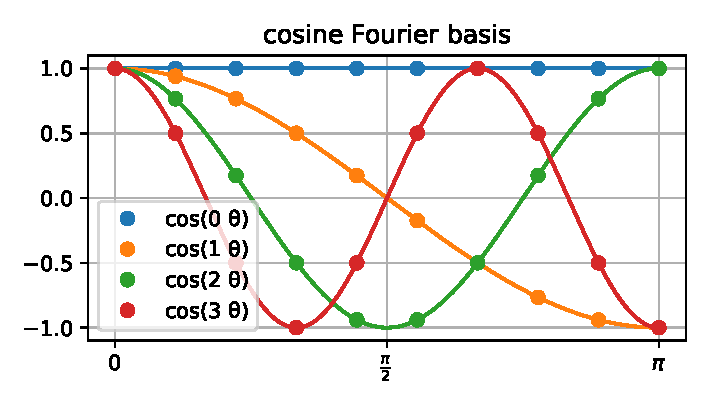
\includegraphics{img/poloidal_Fourier_basis.pdf}
  \caption{The first four poloidal cosine Fourier basis functions for $n_{\theta,2} = 10$.}
  \label{fig:poloidal_Fourier_basis}
\end{figure}

In the example of Fig.~\ref{fig:poloidal_symmetry}, the points at $\theta=0$ and at $\theta=\pi$ appear only once
for the even-parity quantity~$R$ in the example and all other value for $R$ of the dots appear twice,
as correctly accounted for by the factors in \eqn{f_m_cos}.

We consider $\hat{F}^{X,\mathrm{sin}}_m$ with $m>0$ next:
\begin{align}
 \hat{F}^{X,\mathrm{sin}}_m
  =&\, \frac{2}{\pi} \int\limits_0^{\pi} F^{X}(\theta) \sin(m \theta) \,\mathrm{d}\theta
  \approx \frac{2}{\pi} \sum\limits_{l=0}^{n_{\theta,2}-1} F^{X}(\theta_l) \sin(m \theta_l) \Delta\theta \begin{cases}
                                                                                                           1/2 &: l=0 \textrm{ or } l=n_{\theta,2}-1 \\
                                                                                                           1   &: \textrm{else}
                                                                                                         \end{cases} \nonumber \\
  =&\, \frac{2}{\bcancel{\pi}} \frac{\bcancel{\pi}}{n_{\theta,2}-1} \sum\limits_{l=1}^{n_{\theta,2}-2} F^{X}(\theta_l) \sin(m \theta_l)
  =    \frac{1}{n_{\theta,2}-1} 2 \sum\limits_{l=0}^{n-1} F^{X}(\theta_l) \sin\left(\frac{\pi}{n+1} \,m \,(l+1) \right)
\end{align}
for $n=n_{\theta,2}-2$.
The first and the last terms in the sum dropped out since $\sin(m 0) = 0$ and $\sin(m \pi) = 0$ at those indices, respectively.
Then, an index shift of $l \rightarrow l-1$ was performed in the sum.

The Fourier transforms are computed in the Fortran implementation of VMEC using
a setup of the Fourier transforms as a matrix-vector multiplication.
Two-dimensional arrays \texttt{cosmui} and \texttt{sinmui} are defined with:
\begin{align}
  \texttt{cosmui}(l,m) =&\, \frac{\texttt{mscale}(m)}{n_\zeta (n_{\theta,2}-1)} \cos\left(\frac{\pi}{n_{\theta,1}} \,m \,l\right) \begin{cases}
                                                                                                                          1/2 &: l=0 \textrm{ or } l=n_{\theta,2}-1 \\
                                                                                                                          1   &: \textrm{else}
                                                                                                                        \end{cases} \\
  \texttt{sinmui}(l,m) =&\, \frac{\texttt{mscale}(m)}{n_\zeta (n_{\theta,2}-1)} \sin\left(\frac{\pi}{n_{\theta,1}} \,m \,l\right)
\end{align}
(in case of \texttt{sinmui}, no attempt is made to trapezoidally-scale the first and last entries along the $l$-dimension, since those are zero anyway)
and a one-dimensional array~\texttt{mscale} with:
\begin{equation}
  \texttt{mscale}(m) = \begin{cases}
                               1  &: m=0           \\
                         \sqrt{2} &: \textrm{else}
                       \end{cases}
\end{equation}
for $l=0,1, ..., (n_{\theta,2}-1)$ and $m=0,1, ..., M$.
The normalization factor is called~\texttt{dnorm} in the code:
\begin{equation}
  \texttt{dnorm} = \frac{1}{n_\zeta (n_{\theta,2}-1)} \, .
\end{equation}
It also contains the normalization factor for the toroidal Fourier integrals (see below).
The computation of $\hat{F}^{X,\mathrm{cos}}_m$ for $m\geq0$ can then be formulated as follows:
\begin{equation}
  \hat{F}^{X,\mathrm{cos}}_m = \sum\limits_{l=0}^{n_{\theta,2}-1} F^{X}(\theta_l) \, \texttt{cosmui}(l,m) \, .
\end{equation}
Note that a factor of $\sqrt{2}$ is missing for $m>0$ to recover \eqn{f_m_cos}.
In turn, if the Fourier transforms are computed using, e.g., FFTW (which implements above transform as \texttt{REDFT00}),
a factor of $1/\sqrt{2}$ has to be applied to the results from that FFT in order to recover the custom VMEC scaling.
Similarly, the computation of $\hat{F}^{X,\mathrm{sin}}_m$ is done as follows:
\begin{equation}
  \hat{F}^{X,\mathrm{sin}}_m = \sum\limits_{l=0}^{n_{\theta,2}-1} F^{X}(\theta_l) \, \texttt{sinmui}(l,m) \, .
\end{equation}
This can be replaced by FFTW's \texttt{RODFT00}, where the first and last points have to be left out explicitly,
the Fourier coefficients are shifted by 1 along the $m$-direction and a factor of $1/\sqrt{2}$ has to be multiplied in as well.
%
% {\color{red} TODO: figure out why exactly mscale, nscale have those particular forms, i.e.,
%  where is made use of the explicit orthogonality with constant factor 0.5?}
%
The poloidal derivatives are implemented using additional matrices:
\begin{align}
  \texttt{cosmumi}(l,m) =&\, (\phantom{-} m) \, \texttt{cosmui}(l,m) \\
  \texttt{sinmumi}(l,m) =&\, (         -  m) \, \texttt{sinmui}(l,m) \, .
\end{align}

\begin{figure}[htbp]
  \centering
  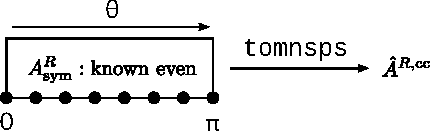
\includegraphics{img/A_R_sym.pdf}
  \caption{Assembly of the Fourier coefficients~$\hat{A}^{R,\mathrm{cc}}$
    from the $A^R$~real-space force component in the symmetric case.}
  \label{fig:A_R_sym}
\end{figure}

\begin{figure}[htbp]
  \centering
  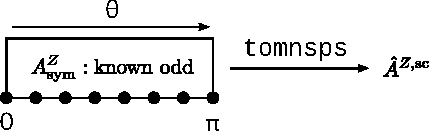
\includegraphics{img/A_Z_sym.pdf}
  \caption{Assembly of the Fourier coefficients~$\hat{A}^{Z,\mathrm{sc}}$
    from the $A^Z$~real-space force component in the symmetric case.}
  \label{fig:A_Z_sym}
\end{figure}

\begin{figure}[htbp]
  \centering
  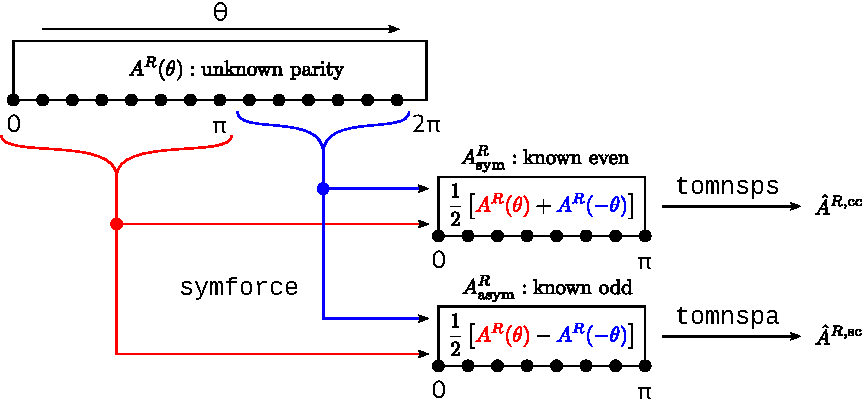
\includegraphics{img/A_R_asym.pdf}
  \caption{Assembly of the Fourier coefficients~$\hat{A}^{R,\mathrm{cc}}$ and~$\hat{A}^{R,\mathrm{sc}}$
    from the $A^R$~real-space force component in the asymmetric/general case.}
  \label{fig:A_R_asym}
\end{figure}

\begin{figure}[htbp]
  \centering
  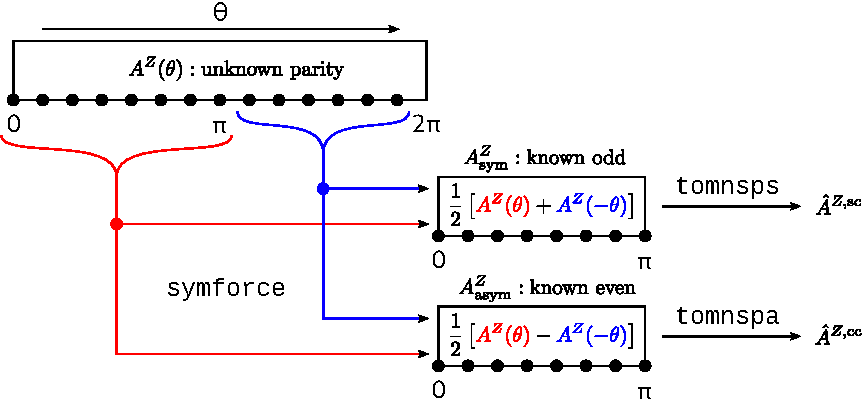
\includegraphics{img/A_Z_asym.pdf}
  \caption{Assembly of the Fourier coefficients~$\hat{A}^{Z,\mathrm{sc}}$ and~$\hat{A}^{Z,\mathrm{cc}}$
    from the $A^Z$~real-space force component in the asymmetric/general case.}
  \label{fig:A_Z_asym}
\end{figure}

\FloatBarrier
Now we turn to the three-dimensional (Stellarator-)symmetric case.
The toroidal Fourier transform can be ignored in the two-dimensional case, since $n_\zeta=1$ and $n=0$,
leading to basis functions $\cos(n\zeta_k)=1$ and $\sin(n\zeta_k)=0$ for the only toroidal grid point at $k=0$.
This effectively disables/removes the toroidal Fourier transform from the setup.
Stellarator symmetry manifests itself as the following parity property
for $R$ and $Z$ of the flux surface geometry under reversal
of both the poloidal $\theta$~coordinate and the toroidal $\zeta$~coordinate:
\begin{align}
  R(-\theta, -\zeta) =&\, \phantom{-}~ R(\theta, \zeta) \\
  Z(-\theta, -\zeta) =&\,          -   Z(\theta, \zeta) \, .
\end{align}
Any other quantity with even (odd) parity has the same symmetry property as $R$ ($Z$) in above equations.

The toroidal grid points (on which the toroidal Fourier transform integrals are discretized)
are distributed evenly in the toroidal direction over the first field period.
The toroidal coordinate~$\zeta$ spans $[0,2\pi[$ over one field period.
This corresponds to $\phi \in [0,2\pi/n_\mathrm{fp}[$ in the underlying cylindrical coordinate system
(recall $\zeta = n_\mathrm{fp} \phi \Leftrightarrow \phi = \zeta / n_\mathrm{fp}$).
It follows for some quantity~$C$ with even parity:
\begin{align}
    C(\zeta) = \sum_{n=0}^{N} \hat{C}_n \cos(n \zeta)
  \Leftrightarrow&\,
    C(\phi ) = \sum_{n=0}^{N} \hat{C}_n \cos(n \,n_\mathrm{fp} \phi) \nonumber \\
    \Rightarrow
    \frac{\partial C}{\partial \zeta} (\zeta) = \sum_{n=0}^{N} (-n              ) \hat{C}_n \sin(n               \zeta)
  \Leftrightarrow&\,
    \frac{\partial C}{\partial \phi } (\phi ) = \sum_{n=0}^{N} (-n \,n_\mathrm{fp}) \hat{C}_n \sin(n \,n_\mathrm{fp} \phi ) \, ,
\end{align}
since
\begin{equation}
  \frac{\partial C}{\partial \phi} = \frac{\partial C}{\partial \zeta} \underbrace{\frac{\partial \zeta}{\partial \phi}}_{=\,n_\mathrm{fp}} (\phi) \, .
\end{equation}

Generally, the argument of the Fourier basis functions is $(m \theta - n \,n_\mathrm{fp} \zeta)$.
Evaluation is done only in the first field period: $\phi \in [0,2\pi/n_\mathrm{fp}[ \Rightarrow \zeta \in [0,2\pi[$.
The argument $(m \theta - n \zeta)$ is used for evaluating the basis functions
on a regular grid in $\zeta$, since no explicit factors of $n_\mathrm{fp}$ occur then.
Toroidal derivatives are to be taken with respect to $\phi$ though,
so the factor to be used in the Fourier sums still is $n \,n_\mathrm{fp}$.

Consider first the Fourier transform of some $2 \pi$-periodic function $f$ of the toroidal coordinate $\zeta$.
Its Fourier coefficients are computed as follows:
\begin{align}
  \hat{f}^\mathrm{cos}_0
  =&\, \frac{1}{2 \pi} \int\limits_0^{2\pi} f(\zeta) \,\mathrm{d}\zeta
    \approx \frac{1}{2 \pi} \sum\limits_{k=0}^{n_\zeta-1} f(\zeta_k) \Delta \zeta
  = \frac{1}{\bcancel{2 \pi}} \frac{\bcancel{2 \pi}}{n_\zeta} \sum\limits_{k=0}^{n_\zeta-1} f(\zeta_k)
  = \frac{1}{n_\zeta} \sum\limits_{k=0}^{n_\zeta-1} f\left(2 \pi \frac{k}{n_\zeta}\right) \\
  \hat{f}^\mathrm{cos}_n
  =&\, \frac{1}{\pi} \int\limits_0^{2\pi} f(\zeta) \cos(n \zeta) \,\mathrm{d}\zeta
    \approx \frac{1}{\pi} \sum\limits_{k=0}^{n_\zeta-1} f(\zeta_k) \cos(n \zeta_k) \Delta \zeta
  = \frac{1}{\bcancel{\pi}} \frac{2 \bcancel{\pi}}{n_\zeta} \sum\limits_{k=0}^{n_\zeta-1} f(\zeta_k) \cos(n \zeta_k) \nonumber \\
  =&\, \frac{2}{n_\zeta} \sum\limits_{k=0}^{n_\zeta-1} f\left(2 \pi \frac{k}{n_\zeta}\right) \cos\left(2 \pi n \frac{k}{n_\zeta}\right) \\
  \hat{f}^\mathrm{sin}_n
  =&\, \frac{1}{\pi} \int\limits_0^{2\pi} f(\zeta) \sin(n \zeta) \,\mathrm{d}\zeta
    \approx \frac{1}{\pi} \sum\limits_{k=0}^{n_\zeta-1} f(\zeta_k) \sin(n \zeta_k) \Delta \zeta
  = \frac{1}{\bcancel{\pi}} \frac{2 \bcancel{\pi}}{n_\zeta} \sum\limits_{k=0}^{n_\zeta-1} f(\zeta_k) \sin(n \zeta_k) \nonumber \\
  =&\, \frac{2}{n_\zeta} \sum\limits_{k=0}^{n_\zeta-1} f\left(2 \pi \frac{k}{n_\zeta}\right) \sin\left(2 \pi n \frac{k}{n_\zeta}\right)
\end{align}
with
\begin{equation}
  \Delta \zeta = \frac{2 \pi}{n_\zeta}
  \textrm{ and }
  \zeta_k = k \, \Delta \zeta = 2 \pi \frac{k}{n_\zeta} \, .
\end{equation}
The Fourier basis functions in the toroidal direction are pre-evaluated
on a regular grid in the toroidal coordinate:
\begin{align}
  \texttt{cosnv}(k,n) =&\, \texttt{nscale}(n) \cos\left(\frac{2 \pi}{n_\zeta} \,n \,k\right) \\
  \texttt{sinnv}(k,n) =&\, \texttt{nscale}(n) \sin\left(\frac{2 \pi}{n_\zeta} \,n \,k\right)
\end{align}
with
\begin{equation}
  \texttt{nscale}(n) = \begin{cases}
                               1  &: n=0           \\
                         \sqrt{2} &: \textrm{else}
                       \end{cases}
\end{equation}
for $k=0,1, ..., (n_\zeta-1)$ and $n=0,1, ..., N$.
Furthermore, the toroidal derivatives are implemented with separate matrices:
\begin{align}
  \texttt{cosnvn}(k,n) =&\, \texttt{nscale}(n) (\phantom{-} n \,n_\mathrm{fp}) \cos\left(\frac{2 \pi}{n_\zeta} \,n \,k\right) \\
  \texttt{sinnvn}(k,n) =&\, \texttt{nscale}(n) (         -  n \,n_\mathrm{fp}) \sin\left(\frac{2 \pi}{n_\zeta} \,n \,k\right) \, .
\end{align}
The computation of the toroidal Fourier integrals $\hat{F}^{X,\mathrm{cos}}_n$ for $n\geq0$ can then be formulated as follows:
\begin{equation}
  \hat{F}^{X,\mathrm{cos}}_n = \sum\limits_{k=0}^{n_\zeta-1} F^{X}(\zeta_k) \, \texttt{cosnv}(k,n) \, .
\end{equation}
Note that also here a factor of $\sqrt{2}$ is missing for $n>0$ to recover the usual Fourier integrals.
Similarly, the computation of $\hat{F}^{X,\mathrm{sin}}_n$ is done as follows:
\begin{equation}
  \hat{F}^{X,\mathrm{sin}}_n = \sum\limits_{k=0}^{n_\zeta-1} F^{X}(\zeta_k) \, \texttt{sinnv}(k,n) \, .
\end{equation}
The general two-dimensional Fourier integrals are assembled
as products of the corresponding one-dimensional transforms:
\begin{align}
  \hat{F}^{X,\mathrm{cc}}_{mn} =&\, \sum\limits_{k=0}^{n_\zeta-1} \sum\limits_{l=0}^{n_{\theta,2}-1} F^{X}(\zeta_k, \theta_l) \, \texttt{cosmui}(l,m) \, \texttt{cosnv}(k,n) \\
  \hat{F}^{X,\mathrm{ss}}_{mn} =&\, \sum\limits_{k=0}^{n_\zeta-1} \sum\limits_{l=0}^{n_{\theta,2}-1} F^{X}(\zeta_k, \theta_l) \, \texttt{sinmui}(l,m) \, \texttt{sinnv}(k,n) \\
  \hat{F}^{X,\mathrm{sc}}_{mn} =&\, \sum\limits_{k=0}^{n_\zeta-1} \sum\limits_{l=0}^{n_{\theta,2}-1} F^{X}(\zeta_k, \theta_l) \, \texttt{sinmui}(l,m) \, \texttt{cosnv}(k,n) \\
  \hat{F}^{X,\mathrm{cs}}_{mn} =&\, \sum\limits_{k=0}^{n_\zeta-1} \sum\limits_{l=0}^{n_{\theta,2}-1} F^{X}(\zeta_k, \theta_l) \, \texttt{cosmui}(l,m) \, \texttt{sinnv}(k,n) \, .
\end{align}
The tangential derivatives are now also easy to assemble.
First consider the poloidal derivatives:
\begin{align}
  \hat{B}^{X,\mathrm{cc}}_{mn} =&\, \sum\limits_{k=0}^{n_\zeta-1} \sum\limits_{l=0}^{n_{\theta,2}-1} B^{X}(\zeta_k, \theta_l) \, \texttt{cosmumi}(l,m) \, \texttt{cosnv}(k,n) \\
  \hat{B}^{X,\mathrm{ss}}_{mn} =&\, \sum\limits_{k=0}^{n_\zeta-1} \sum\limits_{l=0}^{n_{\theta,2}-1} B^{X}(\zeta_k, \theta_l) \, \texttt{sinmumi}(l,m) \, \texttt{sinnv}(k,n) \\
  \hat{B}^{X,\mathrm{sc}}_{mn} =&\, \sum\limits_{k=0}^{n_\zeta-1} \sum\limits_{l=0}^{n_{\theta,2}-1} B^{X}(\zeta_k, \theta_l) \, \texttt{sinmumi}(l,m) \, \texttt{cosnv}(k,n) \\
  \hat{B}^{X,\mathrm{cs}}_{mn} =&\, \sum\limits_{k=0}^{n_\zeta-1} \sum\limits_{l=0}^{n_{\theta,2}-1} B^{X}(\zeta_k, \theta_l) \, \texttt{cosmumi}(l,m) \, \texttt{sinnv}(k,n) \, .
\end{align}
Next consider the toroidal derivatives:
\begin{align}
  \hat{C}^{X,\mathrm{cc}}_{mn} =&\, \sum\limits_{k=0}^{n_\zeta-1} \sum\limits_{l=0}^{n_{\theta,2}-1} C^{X}(\zeta_k, \theta_l) \, \texttt{cosmui}(l,m) \, \texttt{cosnvn}(k,n) \\
  \hat{C}^{X,\mathrm{ss}}_{mn} =&\, \sum\limits_{k=0}^{n_\zeta-1} \sum\limits_{l=0}^{n_{\theta,2}-1} C^{X}(\zeta_k, \theta_l) \, \texttt{sinmui}(l,m) \, \texttt{sinnvn}(k,n) \\
  \hat{C}^{X,\mathrm{sc}}_{mn} =&\, \sum\limits_{k=0}^{n_\zeta-1} \sum\limits_{l=0}^{n_{\theta,2}-1} C^{X}(\zeta_k, \theta_l) \, \texttt{sinmui}(l,m) \, \texttt{cosnvn}(k,n) \\
  \hat{C}^{X,\mathrm{cs}}_{mn} =&\, \sum\limits_{k=0}^{n_\zeta-1} \sum\limits_{l=0}^{n_{\theta,2}-1} C^{X}(\zeta_k, \theta_l) \, \texttt{cosmui}(l,m) \, \texttt{sinnvn}(k,n) \, .
\end{align}
This completes the Fourier transforms of the force components in VMEC.


% TODO: residue() and all the rest until convergence



\section{Output Quantities}
After VMEC has converged, the output quantities are computed.
These are the arrays etc. that eventually end up in the output files.

The \texttt{wout} file is always written.
Also, the logging part of the \texttt{threed1} file is always written.
All other output files are only written if VMEC ended because ...
\begin{enumerate}
 \item ... it converged to the desired force tolerance, or because
 \item ... the number of allowed iterations was exceeded
\end{enumerate}
and are omitted if VMEC failed for any other reason.

The interface between the equilibrium computation and the output quantities
is a little bit weird.
At the beginning of the \texttt{fileout} subroutine that controls the computation
of the output quantities as well as the creation of the output files,
the ideal MHD forward model within VMEC (\texttt{funct3d}) is run again,
but with the global flag \texttt{iequi} set to 1 now (instead of the regular value of 0).
%
This is required, since many arrays are re-used within VMEC during the iterations
and this would overwrite quantities that are still needed for the output quantities.

In case of a bad Jacobian, the evaluation of the forward model
is terminated after the Jacobian has been computed.
This means that the geometry in the wout file will refer to the intersecting flux surfaces
that triggered the Jacobian error,
but the magnetic field components etc. will refer to the previous iteration.
% TODO: check this!

In summary, if VMEC did not converge properly, don't use the output quantities for anything!

The final forward model evaluation stops
before updating the radial preconditioner.

\subsection{Preparation of the internal data}
The covariant magnetic field component~$B_\zeta$ is averaged back onto the half-grid.
The scheme used for that is illustrated in Fig.~\ref{fig:bsubv_mesh_blending}.
\begin{figure}[htbp]
 \centering
 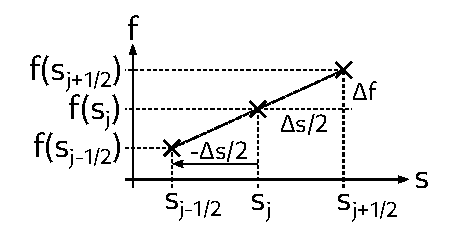
\includegraphics{img/bsubv_mesh_blending.pdf}
 \caption{Linear interpolation scheme used for mesh blending of $B_\zeta$.}
 \label{fig:bsubv_mesh_blending}
\end{figure}
Assume that a function~$f$ is given on a full-grid point $s_j$ and the outward half-grid point~$s_{j+\half}$.
Then, linear extrapolation can be used to compute $f$ at $s_{j-\half}$:
\begin{equation}
 f(s_{j-\half}) \approx f(s_j) + (- \Delta s / 2) \frac{\partial f}{\partial s}\vert_{s=s_j} \label{eqn:linear_extrap} \, .
\end{equation}
The radial derivative of $f$ can be approximated using finite differences:
\begin{equation}
 \frac{\partial f}{\partial s}\vert_{s=s_j}
 \approx
 \frac{f(s_{j+\half}) - f(s_j)}{\Delta s / 2} \, .
\end{equation}
Putting this back into \eqn{linear_extrap} leads to:
\begin{align}
 f(s_{j-\half}) \approx&\, f(s_j) - \bcancel{\Delta s / 2} \frac{f(s_{j+\half}) - f(s_j)}{\bcancel{\Delta s / 2}} \nonumber \\
   ~                =&\, 2 f(s_j) - f(s_{j+\half}) \, .
\end{align}
This can be computed conveniently in-place when starting the radial loop out at the LCFS.

In the next step, the poloidal current is restored by adjusting the offset in~$B_\zeta$.
The poloidal current~$I_\textrm{pol}$ is defined as the average value of $B_\zeta$ over a flux surface:
\begin{equation}
 I_\textrm{pol} = \langle B_\zeta \rangle \, .
\end{equation}
After above mesh blending, the poloidal current is corrected back to its original value,
which was computed during the iterations:
\begin{align}
 B_\zeta \leftarrow&\, B_\zeta - \left[ \langle B_\zeta \rangle - I_\textrm{pol}^\textrm{ref} \right] \nonumber \\
     ~            =&\, B_\zeta + \underbrace{\left[ I_\textrm{pol}^\textrm{ref} - \langle B_\zeta \rangle \right]}_{=\texttt{curpol\_temp}} \, ,
\end{align}
where $I_\textrm{pol}^\textrm{ref}$ is the targeted poloidal current.

The toroidal magnetic flux profile is re-computed with the correct normalization and sign
by quadrature from its radial derivative:
\begin{equation}
 \Phi(s_j) = \texttt{signgs} \cdot 2 \pi \cdot \frac{1}{\Delta s} \sum\limits_{j'=0}^{j} \Phi'(s_{j'})
\end{equation}

\subsection{Computation of $B_s$}
The covariant component~$B_s$ of the magnetic field is computed now
based on the contravariant magnetic field components on the half-grid:
\begin{equation}
 B_s(s_{j+\half}, \zeta_k, \theta_l) = \left[B^\theta g_{s \theta} + B^\zeta g_{s \zeta} \right](s_{j+\half}, \zeta_k, \theta_l) \, .
\end{equation}
The metric elements $g_{s \theta}$ and $g_{s \zeta}$ are computed as follows:
\begin{align}
 g_{s \theta} =&\, R_s R_\theta + Z_s Z_\theta \\
 g_{s \zeta}  =&\, R_s R_\zeta  + Z_s Z_\zeta  \, .
\end{align}
The radial derivatives are computed based on the quantities $\tilde{R_s}$ and $\tilde{Z_s}$
that are already available from the computation of the Jacobian:
\begin{align}
 R_s(s_{j+\half}) =&\, \tilde{R_s}(s_{j+\half}) + \frac{1}{2 \sqrt{s_{j+\half}}} R^\textrm{o}(s_{j+\half}) \\
 Z_s(s_{j+\half}) =&\, \tilde{Z_s}(s_{j+\half}) + \frac{1}{2 \sqrt{s_{j+\half}}} Z^\textrm{o}(s_{j+\half})
\end{align}
with
\begin{align}
 R^\textrm{o}(s_{j+\half}) =&\, \frac{1}{2} \left[ R^\textrm{o}(s_{j+1}) + R^\textrm{o}(s_j) \right] \\
 Z^\textrm{o}(s_{j+\half}) =&\, \frac{1}{2} \left[ Z^\textrm{o}(s_{j+1}) + Z^\textrm{o}(s_j) \right] \, .
\end{align}
The derivatives in the toroidal direction, $R_\zeta$ and $Z_\zeta$,
are taken as zero in the case of an axisymmetric equilibrium calculation.
Otherwise, they are interpolated from the even-$m$ and odd-$m$ contributions
that are available on the full-grid from the inverse-DFTs:
\begin{align}
 R_\zeta(s_{j+\half}) =&\, R_\zeta^\textrm{e}(s_{j+\half}) + \sqrt{s_{j+\half}} R_\zeta^\textrm{o}(s_{j+\half}) \\
 Z_\zeta(s_{j+\half}) =&\, Z_\zeta^\textrm{e}(s_{j+\half}) + \sqrt{s_{j+\half}} Z_\zeta^\textrm{o}(s_{j+\half}) \, .
\end{align}
with
\begin{align}
 R_\zeta^\textrm{e}(s_{j+\half}) =&\, \frac{1}{2} \left[ R_\zeta^\textrm{e}(s_{j+1}) + R_\zeta^\textrm{e}(s_j) \right] \\
 R_\zeta^\textrm{o}(s_{j+\half}) =&\, \frac{1}{2} \left[ R_\zeta^\textrm{o}(s_{j+1}) + R_\zeta^\textrm{o}(s_j) \right] \\
 Z_\zeta^\textrm{e}(s_{j+\half}) =&\, \frac{1}{2} \left[ Z_\zeta^\textrm{e}(s_{j+1}) + Z_\zeta^\textrm{e}(s_j) \right] \\
 Z_\zeta^\textrm{o}(s_{j+\half}) =&\, \frac{1}{2} \left[ Z_\zeta^\textrm{o}(s_{j+1}) + Z_\zeta^\textrm{o}(s_j) \right] \, .
\end{align}
Furthermore, the cylindrical components of the magnetic field
are computed on the half-grid:
\begin{align}
 B^R       =&\, B^\theta R_\theta + B^\zeta R_\zeta \\
 B^\varphi =&\, R B^\zeta \\
 B^Z       =&\, B^\theta Z_\theta + B^\zeta Z_\zeta \, .
\end{align}

% \subsection{Low-Pass-Filtering of Covariant Magnetic Field Components}
% TODO

\FloatBarrier
\newpage
\section{Correction of $B_s$}
The radial part of the ideal MHD force balance equation is given in Eqn.~(4d)
of Ref.~\cite{hirshman_whitson_1983}:
\begin{equation}
 F_s = \frac{1}{\mu_0} \left(
     B^\theta  \frac{\partial B_\theta}{\partial s}
   + B^\zeta   \frac{\partial B_\zeta }{\partial s}
   - \mathbf{B} \cdot \nabla B_s
 \right) + p' \, . \label{eqn:f_rho}
\end{equation}
The dot product $\mathbf{B} \cdot \nabla B_s$ has to be expressed
using contravariant components for $\mathbf{B}$,
because $B_s$ is a covariant component:
\begin{align}
 \mathbf{B} \cdot \nabla B_s
 =&\, \begin{pmatrix}
    0 \\
    B^\theta \\
    B^\zeta
   \end{pmatrix}
   \cdot
   \begin{pmatrix}
    \partial B_s / \partial s \\
    \partial B_s / \partial \theta \\
    \partial B_s / \partial \zeta
   \end{pmatrix} \\
 =&\,  B^\theta \frac{\partial B_s}{\partial \theta}
     + B^\zeta \frac{\partial B_s}{\partial \zeta}
\end{align}
where we have already factored in the assumption of nested flux surfaces,
which implies $B^s = 0$.
Using the assumption of an equilibrium being in force balance,
which implies $F_s = 0$,
we can solve \eqn{f_rho} for the terms depending on $B_s$:
\begin{equation}
   B^\theta \frac{\partial B_s}{\partial \theta}
 + B^\zeta \frac{\partial B_s}{\partial \zeta}
 =   B^\theta  \frac{\partial B_\theta}{\partial s}
   + B^\zeta   \frac{\partial B_\zeta }{\partial s}
   + \mu_0 p' \label{eqn:radial_force_balance}
\end{equation}
We now use a Fourier representation for $B_s$,
which has odd parity in case of assuming stellarator symmetry:
\begin{equation}
 B_s(\theta, \zeta) =
 \sum\limits_{\texttt{mn}=0}^{\texttt{mnmax}-1}
   \hat{B}^\textrm{sin}_{s,\texttt{mn}}
   \sin(m_\texttt{mn} \theta - n_\texttt{mn} \zeta) \, .
\end{equation}
This allows to use analytical expressions
for the tangential derivatives of $B_s$:
\begin{align}
 \frac{\partial B_s}{\partial \theta} =&\,
 \sum\limits_{\texttt{mn}=0}^{\texttt{mnmax}-1}
   m \hat{B}^\textrm{sin}_{s,\texttt{mn}}
   \cos(m_\texttt{mn} \theta - n_\texttt{mn} \zeta) \\
 \frac{\partial B_s}{\partial \zeta} =&\,
 \sum\limits_{\texttt{mn}=0}^{\texttt{mnmax}-1}
   -n \hat{B}^\textrm{sin}_{s,\texttt{mn}}
   \cos(m_\texttt{mn} \theta - n_\texttt{mn} \zeta) \, .
\end{align}
We want to solve \eqn{radial_force_balance} for the Fourier coefficients of $B_s$
on all real-space grid points $\texttt{kl}$ at the same time.
This can be facilitated by formulating \eqn{radial_force_balance}
as a linear system of equations ($\mathbf{A} \mathbf{x} = \mathbf{b}$):
\begin{align}
  \underbrace{
  \left(
    (  m_\texttt{mn} B^\theta_\texttt{kl}
     - n_\texttt{mn} B^\zeta_\texttt{kl} )
     \cos(  m_\texttt{mn} \theta_\texttt{kl}
          - n_\texttt{mn} \zeta_\texttt{kl})
  \right)
  }_{\equiv \mathbf{A}}
  \underbrace{
    \hat{B}^\textrm{sin}_{s,\texttt{mn}}
  }_{\equiv \mathbf{x}}
  =
  \underbrace{
    \left(
       B^\theta  \frac{\partial B_\theta}{\partial s}
     + B^\zeta   \frac{\partial B_\zeta }{\partial s}
     + \mu_0 p'
    \right)_\texttt{kl}
  }_{\equiv \mathbf{b}}
\end{align}
for all grid points indexed by \texttt{kl}.
Summation over \texttt{mn} is implied.

Typically, the real-space resolution
(number of grid points in poloidal and toroidal direction)
is larger than the number of Fourier coefficients,
which implies that the linear system of equations
is over-constrained and hence needs to be
solved in a least-squares sense.

\subsection{Mercier Stability}

The contribution due to magnetic shear is computed as follows:
\begin{align}
 D_\textrm{shear} = (\iota')^2 / 4 \, .
\end{align}
%
The contribution due to the plasma current is computed as follows:
\begin{align}
 D_\textrm{curr} = -\iota' (t_{jb} - I_\textrm{tor}' t_{bb}) \, .
\end{align}
%
The contribution due to the magnetic well is computed as follows:
\begin{align}
 D_\textrm{well} = p' (V'' - p' t_{pp}) t_{bb} \, .
\end{align}
%
The contribution due to geodesic curvature is computed as follows:
\begin{align}
 D_\textrm{geod} = t_{jb}^2 - t_{bb} t_{jj} \, .
\end{align}
%
The final value for Mercier's stability criterion is then added up from the four contributions:
\begin{align}
 D_\textrm{Merc} = D_\textrm{shear} + D_\textrm{curr} + D_\textrm{well} + D_\textrm{geod}\, .
\end{align}
